% Chapter 13: Foundation models and conformal prediction
% Advanced Time Series Analysis and Forecasting -- Master's programme Applied Statistics and Data Science, year 1, semester 2, Bucharest University of Economic Studies
% GENERATED by latex/build_chapter13.py -- edit the generator, not this file.

\newcommand{\coursename}{Advanced Time Series Analysis and Forecasting}
% Preambul comun ATS -- Analiza avansată a seriilor de timp și previziune / Advanced Time Series Analysis and Forecasting
% (Beamer, 16:9). Același design ca MFM, SFM și TSA (copiat din TSA, 5 octombrie 2026). Înainte de % Preambul comun ATS -- Analiza avansată a seriilor de timp și previziune / Advanced Time Series Analysis and Forecasting
% (Beamer, 16:9). Același design ca MFM, SFM și TSA (copiat din TSA, 5 octombrie 2026). Înainte de % Preambul comun ATS -- Analiza avansată a seriilor de timp și previziune / Advanced Time Series Analysis and Forecasting
% (Beamer, 16:9). Același design ca MFM, SFM și TSA (copiat din TSA, 5 octombrie 2026). Înainte de \input{../../latex/preamble} se definește
%   \newcommand{\coursename}{Advanced Time Series Analysis and Forecasting}          (EN)
%   \newcommand{\coursename}{Analiza avansată a seriilor de timp și previziune}       (RO)  și  \def\atslang{ro}
% Fișierele .tex se află în EN/Courses, EN/Seminars, RO/Cursuri, RO/Seminarii (două niveluri sub rădăcină).
% Deck-urile sînt generate de latex/build_chapterN.py / build_seminarN.py (vezi latex/ats_build.py).

\documentclass[9pt, aspectratio=169, t]{beamer}
\providecommand{\coursename}{Advanced Time Series Analysis and Forecasting}

% Ensure content fits on slides
\setbeamersize{text margin left=8mm, text margin right=8mm}
% Smaller institute font (title page)
\setbeamerfont{institute}{size=\footnotesize}

%=============================================================================
% THEME AND STYLE CONFIGURATION
%=============================================================================
\usetheme{default}
% Using default theme for clean header/footer control

% Color Palette (matching Redispatch PDF)
\definecolor{MainBlue}{RGB}{26, 58, 110}
\definecolor{AccentBlue}{RGB}{26, 58, 110}
\definecolor{IDAred}{RGB}{205, 0, 0}
\definecolor{DarkGray}{RGB}{51, 51, 51}
\definecolor{MediumGray}{RGB}{128, 128, 128}
\definecolor{LightGray}{RGB}{248, 248, 248}
\definecolor{VeryLightGray}{RGB}{235, 235, 235}
\definecolor{KeynoteGray}{RGB}{218, 218, 218}
\definecolor{SectionGray}{RGB}{120, 120, 120}
\definecolor{FooterGray}{RGB}{100, 100, 100}
\definecolor{Crimson}{RGB}{220, 53, 69}
\definecolor{Forest}{RGB}{46, 125, 50}
\definecolor{Amber}{RGB}{181, 133, 63}
\definecolor{Orange}{RGB}{230, 126, 34}
\definecolor{Purple}{RGB}{142, 68, 173}

% Gradient background (exact Keynote 315° gradient: white to RGB 218,218,218)
\setbeamertemplate{background}{%
    \begin{tikzpicture}[remember picture, overlay]
        \shade[shading=axis, shading angle=315,
        top color=white, bottom color=KeynoteGray]
        (current page.south west) rectangle (current page.north east);
    \end{tikzpicture}%
}
% Fallback solid color for compatibility
\setbeamercolor{background canvas}{bg=}

\setbeamercolor{palette primary}{bg=MainBlue, fg=white}
\setbeamercolor{palette secondary}{bg=MainBlue!85, fg=white}
\setbeamercolor{palette tertiary}{bg=MainBlue!70, fg=white}
\setbeamercolor{structure}{fg=MainBlue}
\setbeamercolor{title}{fg=IDAred}
\setbeamercolor{frametitle}{fg=IDAred, bg=}
\setbeamercolor{block title}{bg=MainBlue, fg=white}
\setbeamercolor{block body}{bg=VeryLightGray, fg=DarkGray}
\setbeamercolor{block title alerted}{bg=Crimson, fg=white}
\setbeamercolor{block body alerted}{bg=Crimson!8, fg=DarkGray}
\setbeamercolor{block title example}{bg=Forest, fg=white}
\setbeamercolor{block body example}{bg=Forest!8, fg=DarkGray}
\setbeamercolor{item}{fg=MainBlue}

% Footer colors (override Madrid theme blue)
\setbeamercolor{author in head/foot}{fg=FooterGray, bg=}
\setbeamercolor{title in head/foot}{fg=FooterGray, bg=}
\setbeamercolor{date in head/foot}{fg=FooterGray, bg=}
\setbeamercolor{section in head/foot}{fg=FooterGray, bg=}
\setbeamercolor{subsection in head/foot}{fg=FooterGray, bg=}

% Bullet styles (apply everywhere including blocks)
\setbeamertemplate{itemize item}{\color{MainBlue}$\boxdot$}
\setbeamertemplate{itemize subitem}{\color{MainBlue}$\blacktriangleright$}
\setbeamertemplate{itemize subsubitem}{\color{MainBlue}\tiny$\bullet$}
\setbeamertemplate{itemize/enumerate body begin}{\normalsize}
\setbeamertemplate{itemize/enumerate subbody begin}{\normalsize}

% Item spacing - compact style
\setlength{\leftmargini}{10pt}       % Level 1: minimal indent
\setlength{\leftmarginii}{10pt}      % Level 2: minimal additional indent
% Compact list spacing (zero extra space before/after lists in blocks)
\makeatletter
\def\@listi{\leftmargin\leftmargini \topsep 0pt \parsep 0pt \itemsep 0pt}
\def\@listii{\leftmargin\leftmarginii \topsep 0pt \parsep 0pt \itemsep 0pt}
\makeatother

\setbeamertemplate{navigation symbols}{}

%=============================================================================
% CUSTOM HEADLINE
%=============================================================================
\setbeamertemplate{headline}{%
    \vskip10pt%
    \hbox to \paperwidth{%
        \hskip0.5cm%
        {\small\color{FooterGray}\renewcommand{\hyperlink}[2]{##2}\insertsectionhead}%
        \hfill%
        \textcolor{FooterGray}{\small\insertframenumber}%
        \hskip0.5cm%
    }%
    \vskip4pt%
    {\color{FooterGray}\hrule height 0.4pt}%
}

%=============================================================================
% CUSTOM FOOTER
%=============================================================================
\usepackage{fontawesome5}

\setbeamertemplate{footline}{%
    {\color{FooterGray}\hrule height 0.4pt}%
    \vskip4pt%
    \hbox to \paperwidth{%
        \hskip0.5cm%
        \textcolor{FooterGray}{\small\coursename}%
        \hfill%
        \raisebox{-0.1em}{%
            \begin{tikzpicture}[x=0.08em, y=0.08em, line width=0.4pt]
                \draw[FooterGray] (0,3) -- (1,4) -- (2,3.5) -- (3,5) -- (4,4) -- (5,6) -- (6,5.5) -- (7,4) -- (8,5) -- (9,7) -- (10,6) -- (11,5) -- (12,6.5) -- (13,8) -- (14,7) -- (15,6) -- (16,7.5) -- (17,9) -- (18,8) -- (19,7) -- (20,8.5) -- (21,10) -- (22,9) -- (23,8) -- (24,9.5);
            \end{tikzpicture}%
        }%
        \hskip0.5cm%
    }%
    \vskip6pt%
}

%=============================================================================
% PACKAGES
%=============================================================================
\usepackage[utf8]{inputenc}
\DeclareUnicodeCharacter{03B1}{\ensuremath{\alpha}}
\usepackage[T1]{fontenc}
\usepackage{amsmath, amssymb, amsthm}
\usepackage{mathtools}
\usepackage{bm}
\usepackage{tikz}
\usetikzlibrary{arrows.meta, positioning, shapes, calc, decorations.pathreplacing, shadings}
\usepackage{booktabs}
\usepackage{multirow}
\usepackage{array}
\usepackage{graphicx}
\usepackage{animate}
\usepackage{hyperref}
\usepackage{colortbl}
\usepackage{listings}
\lstset{language=Python, basicstyle=\ttfamily\scriptsize, keywordstyle=\color{MainBlue}\bfseries,
  commentstyle=\color{Forest}, stringstyle=\color{Crimson}, breaklines=true,
  frame=none, backgroundcolor=\color{VeryLightGray}, xleftmargin=2mm}
\hypersetup{colorlinks=true, linkcolor=MainBlue, urlcolor=MainBlue}
\graphicspath{{../../logos/}{../../charts/}{../../photos/}}
\usepackage{xcolor}
\hfuzz=2pt  % Suppress tiny overfull warnings (<2pt)
\vfuzz=2pt  % Suppress tiny vertical overfull warnings (<2pt)

%=============================================================================
% QUANTLET COMMANDS
%   \quantlet{<displayed name>}{<url>}       (generic)
%   \atsquantlet{Ch_05}{ATS_ch5_garch}       -> https://github.com/danpele/Advanced-Time-Series/tree/main/Quantlets/Ch_05/ATS_ch5_garch
%   \qlurl{<folder>} is defined per chapter by the generator (Quantlets/Ch_NN/<folder>)
%=============================================================================
\newcommand{\atsrepo}{https://github.com/danpele/Advanced-Time-Series}
\newcommand{\atsqlbase}{https://github.com/danpele/Advanced-Time-Series/tree/main/Quantlets}
\newcommand{\quantlet}[2]{%
    \hfill\href{#2}{%
        \raisebox{-0.15em}{
\includegraphics[height=0.7em]{ql_logo.png}}%
        \textcolor{MainBlue}{\tiny\ #1}%
    }%
}
\newcommand{\atsquantlet}[2]{\quantlet{\detokenize{#2}}{\atsqlbase/#1/#2}}

%=============================================================================
% NOTEBOOKS (Google Colab)
%   \colaburl{notebooks/EN/chapter5_seminar_notebook.ipynb} -> the Colab link of a file in the ATS repo
%   \nb: the chapter notebook (each seminar deck redefines it with \renewcommand)
%=============================================================================
\newcommand{\colaburl}[1]{https://colab.research.google.com/github/danpele/Advanced-Time-Series/blob/main/#1}
\newcommand{\nb}{https://colab.research.google.com/github/danpele/Advanced-Time-Series/tree/main/notebooks/EN}
\newcommand{\nbname}{notebooks/EN}

%=============================================================================
% SLIDE HELPERS (used by the generators; the same as in MFM)
%=============================================================================
% local font size for list bodies (the preamble forces \normalsize)
\newcommand{\itemsize}[1]{\setbeamertemplate{itemize/enumerate body begin}{#1}\setbeamertemplate{itemize/enumerate subbody begin}{#1}}
\newcommand{\intitle}[1]{{\hypersetup{urlcolor=white}#1}}   % white links inside coloured title bars
\newcommand{\imgcap}[1]{{\scriptsize #1}\\[0.5mm]}          % caption under a photo
\newcommand{\imgcredit}[2]{{\tiny\color{FooterGray}\href{#1}{#2}}}   % image credit: source URL, author/licence
\newcommand{\aiprompt}[1]{{\ttfamily\color{MainBlue}#1}}     % a prompt to an AI assistant

%=============================================================================
% SEMINARS: student version by default; the instructor wrapper *_solutions.tex sets \solutionstrue
%=============================================================================
\makeatletter\@ifundefined{ifsolutions}{\expandafter\newif\csname ifsolutions\endcsname}{}\makeatother
\newcommand{\solonly}[1]{\ifsolutions #1\fi}
\newcommand{\propsub}{\ifsolutions\else\framesubtitle{\ifdefined\atslang Rezolvarea se discută la seminar\else Solution discussed in class\fi}\fi}

%=============================================================================
% APPENDIX AND CHAPTER LINKS (latex/appendix_links.py writes the calls; it also re-declares these
% macros before \begin{document}, so the decks compile with or without this preamble block)
%=============================================================================
\providecommand{\atsapplink}[3]{\hypertarget{#2}{}\hyperlink{#1}{\beamergotobutton{#3}}}
\providecommand{\atsappback}[2]{\begin{tikzpicture}[remember picture,overlay]\node[anchor=south east] at ([xshift=-3mm,yshift=7mm]current page.south east){\hyperlink{#1}{\beamerreturnbutton{#2}}};\end{tikzpicture}}
\providecommand{\atschlink}[2]{\href{#1}{#2}}
\providecommand{\atschlinkt}[2]{\href{#1}{\usebeamercolor[fg]{frametitle}#2}}

%=============================================================================
% QUANTINAR COMMAND: link către un curs Quantinar (subiecte avansate)
%=============================================================================
\newcommand{\quantinar}[2]{%
    \href{#2}{%
        \raisebox{-0.15em}{
\includegraphics[height=0.8em]{qr_logo.png}}%
        \textcolor{MainBlue}{\scriptsize\ #1}%
    }%
}

%=============================================================================
% CUSTOM TITLE PAGE
%=============================================================================
\defbeamertemplate*{title page}{hybrid}[1][]
{
    \vspace{0.2cm}
    % Logos row - top header (with clickable links)
    \begin{center}
        \href{https://www.ase.ro}{
\includegraphics[height=1.0cm]{ase_logo.png}}\hspace{0.3cm}%
        \href{https://theida.net}{
\includegraphics[height=1.0cm]{ida_logo.png}}\hspace{0.3cm}%
        \href{https://blockchain-research-center.com}{
\includegraphics[height=1.0cm]{brc_logo.png}}\hspace{0.3cm}%
        \href{https://www.ai4efin.ase.ro}{
\includegraphics[height=1.0cm]{ai4efin_logo.png}}\hspace{0.3cm}%
        \href{https://ipe.ro/new}{
\includegraphics[height=1.0cm]{acad_logo.png}}\hspace{0.3cm}%
        \href{https://www.digital-finance-msca.com}{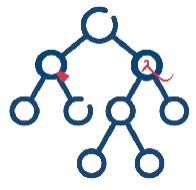
\includegraphics[height=1.0cm]{msca_logo.png}}%
    \end{center}

    \vspace{0.6cm}

    % Main title with Q logos on sides (with clickable links)
    \begin{center}
        \begin{minipage}{0.1\textwidth}
            \centering
            \href{https://quantlet.com}{
\includegraphics[height=1.1cm]{ql_logo.png}}
        \end{minipage}%
        \begin{minipage}{0.78\textwidth}
            \centering
            {\LARGE\bfseries\usebeamercolor[fg]{title}\inserttitle}

            \vspace{0.3cm}

            {\usebeamerfont{subtitle}\usebeamercolor[fg]{title}\insertsubtitle}
        \end{minipage}%
        \begin{minipage}{0.1\textwidth}
            \centering
            \href{https://quantinar.com}{
\includegraphics[height=1.1cm]{qr_logo.png}}
        \end{minipage}
    \end{center}

    \vspace{0.6cm}

    % Authors (left aligned)
    \hspace{0.5cm}{\usebeamerfont{author}\insertauthor}

    \vspace{0.3cm}

    % Institute/Affiliations (left aligned)
    \hspace{0.5cm}\begin{minipage}[t]{0.9\textwidth}
        \raggedright\small\insertinstitute
    \end{minipage}
}

%=============================================================================
% THEOREM ENVIRONMENTS
%=============================================================================
\theoremstyle{definition}
\setbeamertemplate{theorems}[numbered]
\ifdefined\atslang
\newtheorem{defn}{Definiție}
\newtheorem{thm}{Teoremă}
\newtheorem{prop}{Propoziție}
\newtheorem{rmk}{Observație}
\else
\newtheorem{defn}{Definition}
\newtheorem{thm}{Theorem}
\newtheorem{prop}{Proposition}
\newtheorem{rmk}{Remark}
\fi

%=============================================================================
% CENTRED MINIPAGE (no extra vertical space)
%=============================================================================
\newenvironment{cminipage}[1]{%
    \par\noindent\hfill\begin{minipage}{#1}\ignorespaces
}{%
    \end{minipage}\hfill\null\par
}

%=============================================================================
% CUSTOM COMMANDS
%=============================================================================
\newcommand{\E}{\mathbb{E}}
\newcommand{\Var}{\text{Var}}
\newcommand{\Cov}{\text{Cov}}
\newcommand{\Corr}{\text{Corr}}
\newcommand{\R}{\mathbb{R}}
\newcommand{\N}{\mathbb{N}}
\newcommand{\Z}{\mathbb{Z}}
\newcommand{\B}{\mathbf{B}}
\newcommand{\imark}{\textcolor{MainBlue}{\textbullet}}
\newcommand{\RMSE}{\text{RMSE}}
\newcommand{\MAE}{\text{MAE}}
\newcommand{\MAPE}{\text{MAPE}}

% Boldface vector/matrix commands (VAR, VECM, state space)
\newcommand{\bY}{\mathbf{Y}}
\newcommand{\bX}{\mathbf{X}}
\newcommand{\bA}{\mathbf{A}}
\newcommand{\bB}{\mathbf{B}}
\newcommand{\bepsilon}{\boldsymbol{\varepsilon}}
\newcommand{\bSigma}{\boldsymbol{\Sigma}}
\newcommand{\bPhi}{\boldsymbol{\Phi}}
\newcommand{\bGamma}{\boldsymbol{\Gamma}}
\newcommand{\bPi}{\boldsymbol{\Pi}}
\newcommand{\bc}{\mathbf{c}}
\newcommand{\balpha}{\boldsymbol{\alpha}}
\newcommand{\bbeta}{\boldsymbol{\beta}}
\newcommand{\bvarepsilon}{\boldsymbol{\varepsilon}}

% Seminar marks
\newcommand{\correct}{\textcolor{Forest}{\checkmark}}
\newcommand{\incorrect}{\textcolor{Crimson}{\texttimes}}
 se definește
%   \newcommand{\coursename}{Advanced Time Series Analysis and Forecasting}          (EN)
%   \newcommand{\coursename}{Analiza avansată a seriilor de timp și previziune}       (RO)  și  \def\atslang{ro}
% Fișierele .tex se află în EN/Courses, EN/Seminars, RO/Cursuri, RO/Seminarii (două niveluri sub rădăcină).
% Deck-urile sînt generate de latex/build_chapterN.py / build_seminarN.py (vezi latex/ats_build.py).

\documentclass[9pt, aspectratio=169, t]{beamer}
\providecommand{\coursename}{Advanced Time Series Analysis and Forecasting}

% Ensure content fits on slides
\setbeamersize{text margin left=8mm, text margin right=8mm}
% Smaller institute font (title page)
\setbeamerfont{institute}{size=\footnotesize}

%=============================================================================
% THEME AND STYLE CONFIGURATION
%=============================================================================
\usetheme{default}
% Using default theme for clean header/footer control

% Color Palette (matching Redispatch PDF)
\definecolor{MainBlue}{RGB}{26, 58, 110}
\definecolor{AccentBlue}{RGB}{26, 58, 110}
\definecolor{IDAred}{RGB}{205, 0, 0}
\definecolor{DarkGray}{RGB}{51, 51, 51}
\definecolor{MediumGray}{RGB}{128, 128, 128}
\definecolor{LightGray}{RGB}{248, 248, 248}
\definecolor{VeryLightGray}{RGB}{235, 235, 235}
\definecolor{KeynoteGray}{RGB}{218, 218, 218}
\definecolor{SectionGray}{RGB}{120, 120, 120}
\definecolor{FooterGray}{RGB}{100, 100, 100}
\definecolor{Crimson}{RGB}{220, 53, 69}
\definecolor{Forest}{RGB}{46, 125, 50}
\definecolor{Amber}{RGB}{181, 133, 63}
\definecolor{Orange}{RGB}{230, 126, 34}
\definecolor{Purple}{RGB}{142, 68, 173}

% Gradient background (exact Keynote 315° gradient: white to RGB 218,218,218)
\setbeamertemplate{background}{%
    \begin{tikzpicture}[remember picture, overlay]
        \shade[shading=axis, shading angle=315,
        top color=white, bottom color=KeynoteGray]
        (current page.south west) rectangle (current page.north east);
    \end{tikzpicture}%
}
% Fallback solid color for compatibility
\setbeamercolor{background canvas}{bg=}

\setbeamercolor{palette primary}{bg=MainBlue, fg=white}
\setbeamercolor{palette secondary}{bg=MainBlue!85, fg=white}
\setbeamercolor{palette tertiary}{bg=MainBlue!70, fg=white}
\setbeamercolor{structure}{fg=MainBlue}
\setbeamercolor{title}{fg=IDAred}
\setbeamercolor{frametitle}{fg=IDAred, bg=}
\setbeamercolor{block title}{bg=MainBlue, fg=white}
\setbeamercolor{block body}{bg=VeryLightGray, fg=DarkGray}
\setbeamercolor{block title alerted}{bg=Crimson, fg=white}
\setbeamercolor{block body alerted}{bg=Crimson!8, fg=DarkGray}
\setbeamercolor{block title example}{bg=Forest, fg=white}
\setbeamercolor{block body example}{bg=Forest!8, fg=DarkGray}
\setbeamercolor{item}{fg=MainBlue}

% Footer colors (override Madrid theme blue)
\setbeamercolor{author in head/foot}{fg=FooterGray, bg=}
\setbeamercolor{title in head/foot}{fg=FooterGray, bg=}
\setbeamercolor{date in head/foot}{fg=FooterGray, bg=}
\setbeamercolor{section in head/foot}{fg=FooterGray, bg=}
\setbeamercolor{subsection in head/foot}{fg=FooterGray, bg=}

% Bullet styles (apply everywhere including blocks)
\setbeamertemplate{itemize item}{\color{MainBlue}$\boxdot$}
\setbeamertemplate{itemize subitem}{\color{MainBlue}$\blacktriangleright$}
\setbeamertemplate{itemize subsubitem}{\color{MainBlue}\tiny$\bullet$}
\setbeamertemplate{itemize/enumerate body begin}{\normalsize}
\setbeamertemplate{itemize/enumerate subbody begin}{\normalsize}

% Item spacing - compact style
\setlength{\leftmargini}{10pt}       % Level 1: minimal indent
\setlength{\leftmarginii}{10pt}      % Level 2: minimal additional indent
% Compact list spacing (zero extra space before/after lists in blocks)
\makeatletter
\def\@listi{\leftmargin\leftmargini \topsep 0pt \parsep 0pt \itemsep 0pt}
\def\@listii{\leftmargin\leftmarginii \topsep 0pt \parsep 0pt \itemsep 0pt}
\makeatother

\setbeamertemplate{navigation symbols}{}

%=============================================================================
% CUSTOM HEADLINE
%=============================================================================
\setbeamertemplate{headline}{%
    \vskip10pt%
    \hbox to \paperwidth{%
        \hskip0.5cm%
        {\small\color{FooterGray}\renewcommand{\hyperlink}[2]{##2}\insertsectionhead}%
        \hfill%
        \textcolor{FooterGray}{\small\insertframenumber}%
        \hskip0.5cm%
    }%
    \vskip4pt%
    {\color{FooterGray}\hrule height 0.4pt}%
}

%=============================================================================
% CUSTOM FOOTER
%=============================================================================
\usepackage{fontawesome5}

\setbeamertemplate{footline}{%
    {\color{FooterGray}\hrule height 0.4pt}%
    \vskip4pt%
    \hbox to \paperwidth{%
        \hskip0.5cm%
        \textcolor{FooterGray}{\small\coursename}%
        \hfill%
        \raisebox{-0.1em}{%
            \begin{tikzpicture}[x=0.08em, y=0.08em, line width=0.4pt]
                \draw[FooterGray] (0,3) -- (1,4) -- (2,3.5) -- (3,5) -- (4,4) -- (5,6) -- (6,5.5) -- (7,4) -- (8,5) -- (9,7) -- (10,6) -- (11,5) -- (12,6.5) -- (13,8) -- (14,7) -- (15,6) -- (16,7.5) -- (17,9) -- (18,8) -- (19,7) -- (20,8.5) -- (21,10) -- (22,9) -- (23,8) -- (24,9.5);
            \end{tikzpicture}%
        }%
        \hskip0.5cm%
    }%
    \vskip6pt%
}

%=============================================================================
% PACKAGES
%=============================================================================
\usepackage[utf8]{inputenc}
\DeclareUnicodeCharacter{03B1}{\ensuremath{\alpha}}
\usepackage[T1]{fontenc}
\usepackage{amsmath, amssymb, amsthm}
\usepackage{mathtools}
\usepackage{bm}
\usepackage{tikz}
\usetikzlibrary{arrows.meta, positioning, shapes, calc, decorations.pathreplacing, shadings}
\usepackage{booktabs}
\usepackage{multirow}
\usepackage{array}
\usepackage{graphicx}
\usepackage{animate}
\usepackage{hyperref}
\usepackage{colortbl}
\usepackage{listings}
\lstset{language=Python, basicstyle=\ttfamily\scriptsize, keywordstyle=\color{MainBlue}\bfseries,
  commentstyle=\color{Forest}, stringstyle=\color{Crimson}, breaklines=true,
  frame=none, backgroundcolor=\color{VeryLightGray}, xleftmargin=2mm}
\hypersetup{colorlinks=true, linkcolor=MainBlue, urlcolor=MainBlue}
\graphicspath{{../../logos/}{../../charts/}{../../photos/}}
\usepackage{xcolor}
\hfuzz=2pt  % Suppress tiny overfull warnings (<2pt)
\vfuzz=2pt  % Suppress tiny vertical overfull warnings (<2pt)

%=============================================================================
% QUANTLET COMMANDS
%   \quantlet{<displayed name>}{<url>}       (generic)
%   \atsquantlet{Ch_05}{ATS_ch5_garch}       -> https://github.com/danpele/Advanced-Time-Series/tree/main/Quantlets/Ch_05/ATS_ch5_garch
%   \qlurl{<folder>} is defined per chapter by the generator (Quantlets/Ch_NN/<folder>)
%=============================================================================
\newcommand{\atsrepo}{https://github.com/danpele/Advanced-Time-Series}
\newcommand{\atsqlbase}{https://github.com/danpele/Advanced-Time-Series/tree/main/Quantlets}
\newcommand{\quantlet}[2]{%
    \hfill\href{#2}{%
        \raisebox{-0.15em}{
\includegraphics[height=0.7em]{ql_logo.png}}%
        \textcolor{MainBlue}{\tiny\ #1}%
    }%
}
\newcommand{\atsquantlet}[2]{\quantlet{\detokenize{#2}}{\atsqlbase/#1/#2}}

%=============================================================================
% NOTEBOOKS (Google Colab)
%   \colaburl{notebooks/EN/chapter5_seminar_notebook.ipynb} -> the Colab link of a file in the ATS repo
%   \nb: the chapter notebook (each seminar deck redefines it with \renewcommand)
%=============================================================================
\newcommand{\colaburl}[1]{https://colab.research.google.com/github/danpele/Advanced-Time-Series/blob/main/#1}
\newcommand{\nb}{https://colab.research.google.com/github/danpele/Advanced-Time-Series/tree/main/notebooks/EN}
\newcommand{\nbname}{notebooks/EN}

%=============================================================================
% SLIDE HELPERS (used by the generators; the same as in MFM)
%=============================================================================
% local font size for list bodies (the preamble forces \normalsize)
\newcommand{\itemsize}[1]{\setbeamertemplate{itemize/enumerate body begin}{#1}\setbeamertemplate{itemize/enumerate subbody begin}{#1}}
\newcommand{\intitle}[1]{{\hypersetup{urlcolor=white}#1}}   % white links inside coloured title bars
\newcommand{\imgcap}[1]{{\scriptsize #1}\\[0.5mm]}          % caption under a photo
\newcommand{\imgcredit}[2]{{\tiny\color{FooterGray}\href{#1}{#2}}}   % image credit: source URL, author/licence
\newcommand{\aiprompt}[1]{{\ttfamily\color{MainBlue}#1}}     % a prompt to an AI assistant

%=============================================================================
% SEMINARS: student version by default; the instructor wrapper *_solutions.tex sets \solutionstrue
%=============================================================================
\makeatletter\@ifundefined{ifsolutions}{\expandafter\newif\csname ifsolutions\endcsname}{}\makeatother
\newcommand{\solonly}[1]{\ifsolutions #1\fi}
\newcommand{\propsub}{\ifsolutions\else\framesubtitle{\ifdefined\atslang Rezolvarea se discută la seminar\else Solution discussed in class\fi}\fi}

%=============================================================================
% APPENDIX AND CHAPTER LINKS (latex/appendix_links.py writes the calls; it also re-declares these
% macros before \begin{document}, so the decks compile with or without this preamble block)
%=============================================================================
\providecommand{\atsapplink}[3]{\hypertarget{#2}{}\hyperlink{#1}{\beamergotobutton{#3}}}
\providecommand{\atsappback}[2]{\begin{tikzpicture}[remember picture,overlay]\node[anchor=south east] at ([xshift=-3mm,yshift=7mm]current page.south east){\hyperlink{#1}{\beamerreturnbutton{#2}}};\end{tikzpicture}}
\providecommand{\atschlink}[2]{\href{#1}{#2}}
\providecommand{\atschlinkt}[2]{\href{#1}{\usebeamercolor[fg]{frametitle}#2}}

%=============================================================================
% QUANTINAR COMMAND: link către un curs Quantinar (subiecte avansate)
%=============================================================================
\newcommand{\quantinar}[2]{%
    \href{#2}{%
        \raisebox{-0.15em}{
\includegraphics[height=0.8em]{qr_logo.png}}%
        \textcolor{MainBlue}{\scriptsize\ #1}%
    }%
}

%=============================================================================
% CUSTOM TITLE PAGE
%=============================================================================
\defbeamertemplate*{title page}{hybrid}[1][]
{
    \vspace{0.2cm}
    % Logos row - top header (with clickable links)
    \begin{center}
        \href{https://www.ase.ro}{
\includegraphics[height=1.0cm]{ase_logo.png}}\hspace{0.3cm}%
        \href{https://theida.net}{
\includegraphics[height=1.0cm]{ida_logo.png}}\hspace{0.3cm}%
        \href{https://blockchain-research-center.com}{
\includegraphics[height=1.0cm]{brc_logo.png}}\hspace{0.3cm}%
        \href{https://www.ai4efin.ase.ro}{
\includegraphics[height=1.0cm]{ai4efin_logo.png}}\hspace{0.3cm}%
        \href{https://ipe.ro/new}{
\includegraphics[height=1.0cm]{acad_logo.png}}\hspace{0.3cm}%
        \href{https://www.digital-finance-msca.com}{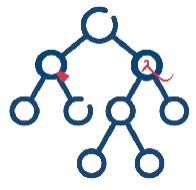
\includegraphics[height=1.0cm]{msca_logo.png}}%
    \end{center}

    \vspace{0.6cm}

    % Main title with Q logos on sides (with clickable links)
    \begin{center}
        \begin{minipage}{0.1\textwidth}
            \centering
            \href{https://quantlet.com}{
\includegraphics[height=1.1cm]{ql_logo.png}}
        \end{minipage}%
        \begin{minipage}{0.78\textwidth}
            \centering
            {\LARGE\bfseries\usebeamercolor[fg]{title}\inserttitle}

            \vspace{0.3cm}

            {\usebeamerfont{subtitle}\usebeamercolor[fg]{title}\insertsubtitle}
        \end{minipage}%
        \begin{minipage}{0.1\textwidth}
            \centering
            \href{https://quantinar.com}{
\includegraphics[height=1.1cm]{qr_logo.png}}
        \end{minipage}
    \end{center}

    \vspace{0.6cm}

    % Authors (left aligned)
    \hspace{0.5cm}{\usebeamerfont{author}\insertauthor}

    \vspace{0.3cm}

    % Institute/Affiliations (left aligned)
    \hspace{0.5cm}\begin{minipage}[t]{0.9\textwidth}
        \raggedright\small\insertinstitute
    \end{minipage}
}

%=============================================================================
% THEOREM ENVIRONMENTS
%=============================================================================
\theoremstyle{definition}
\setbeamertemplate{theorems}[numbered]
\ifdefined\atslang
\newtheorem{defn}{Definiție}
\newtheorem{thm}{Teoremă}
\newtheorem{prop}{Propoziție}
\newtheorem{rmk}{Observație}
\else
\newtheorem{defn}{Definition}
\newtheorem{thm}{Theorem}
\newtheorem{prop}{Proposition}
\newtheorem{rmk}{Remark}
\fi

%=============================================================================
% CENTRED MINIPAGE (no extra vertical space)
%=============================================================================
\newenvironment{cminipage}[1]{%
    \par\noindent\hfill\begin{minipage}{#1}\ignorespaces
}{%
    \end{minipage}\hfill\null\par
}

%=============================================================================
% CUSTOM COMMANDS
%=============================================================================
\newcommand{\E}{\mathbb{E}}
\newcommand{\Var}{\text{Var}}
\newcommand{\Cov}{\text{Cov}}
\newcommand{\Corr}{\text{Corr}}
\newcommand{\R}{\mathbb{R}}
\newcommand{\N}{\mathbb{N}}
\newcommand{\Z}{\mathbb{Z}}
\newcommand{\B}{\mathbf{B}}
\newcommand{\imark}{\textcolor{MainBlue}{\textbullet}}
\newcommand{\RMSE}{\text{RMSE}}
\newcommand{\MAE}{\text{MAE}}
\newcommand{\MAPE}{\text{MAPE}}

% Boldface vector/matrix commands (VAR, VECM, state space)
\newcommand{\bY}{\mathbf{Y}}
\newcommand{\bX}{\mathbf{X}}
\newcommand{\bA}{\mathbf{A}}
\newcommand{\bB}{\mathbf{B}}
\newcommand{\bepsilon}{\boldsymbol{\varepsilon}}
\newcommand{\bSigma}{\boldsymbol{\Sigma}}
\newcommand{\bPhi}{\boldsymbol{\Phi}}
\newcommand{\bGamma}{\boldsymbol{\Gamma}}
\newcommand{\bPi}{\boldsymbol{\Pi}}
\newcommand{\bc}{\mathbf{c}}
\newcommand{\balpha}{\boldsymbol{\alpha}}
\newcommand{\bbeta}{\boldsymbol{\beta}}
\newcommand{\bvarepsilon}{\boldsymbol{\varepsilon}}

% Seminar marks
\newcommand{\correct}{\textcolor{Forest}{\checkmark}}
\newcommand{\incorrect}{\textcolor{Crimson}{\texttimes}}
 se definește
%   \newcommand{\coursename}{Advanced Time Series Analysis and Forecasting}          (EN)
%   \newcommand{\coursename}{Analiza avansată a seriilor de timp și previziune}       (RO)  și  \def\atslang{ro}
% Fișierele .tex se află în EN/Courses, EN/Seminars, RO/Cursuri, RO/Seminarii (două niveluri sub rădăcină).
% Deck-urile sînt generate de latex/build_chapterN.py / build_seminarN.py (vezi latex/ats_build.py).

\documentclass[9pt, aspectratio=169, t]{beamer}
\providecommand{\coursename}{Advanced Time Series Analysis and Forecasting}

% Ensure content fits on slides
\setbeamersize{text margin left=8mm, text margin right=8mm}
% Smaller institute font (title page)
\setbeamerfont{institute}{size=\footnotesize}

%=============================================================================
% THEME AND STYLE CONFIGURATION
%=============================================================================
\usetheme{default}
% Using default theme for clean header/footer control

% Color Palette (matching Redispatch PDF)
\definecolor{MainBlue}{RGB}{26, 58, 110}
\definecolor{AccentBlue}{RGB}{26, 58, 110}
\definecolor{IDAred}{RGB}{205, 0, 0}
\definecolor{DarkGray}{RGB}{51, 51, 51}
\definecolor{MediumGray}{RGB}{128, 128, 128}
\definecolor{LightGray}{RGB}{248, 248, 248}
\definecolor{VeryLightGray}{RGB}{235, 235, 235}
\definecolor{KeynoteGray}{RGB}{218, 218, 218}
\definecolor{SectionGray}{RGB}{120, 120, 120}
\definecolor{FooterGray}{RGB}{100, 100, 100}
\definecolor{Crimson}{RGB}{220, 53, 69}
\definecolor{Forest}{RGB}{46, 125, 50}
\definecolor{Amber}{RGB}{181, 133, 63}
\definecolor{Orange}{RGB}{230, 126, 34}
\definecolor{Purple}{RGB}{142, 68, 173}

% Gradient background (exact Keynote 315° gradient: white to RGB 218,218,218)
\setbeamertemplate{background}{%
    \begin{tikzpicture}[remember picture, overlay]
        \shade[shading=axis, shading angle=315,
        top color=white, bottom color=KeynoteGray]
        (current page.south west) rectangle (current page.north east);
    \end{tikzpicture}%
}
% Fallback solid color for compatibility
\setbeamercolor{background canvas}{bg=}

\setbeamercolor{palette primary}{bg=MainBlue, fg=white}
\setbeamercolor{palette secondary}{bg=MainBlue!85, fg=white}
\setbeamercolor{palette tertiary}{bg=MainBlue!70, fg=white}
\setbeamercolor{structure}{fg=MainBlue}
\setbeamercolor{title}{fg=IDAred}
\setbeamercolor{frametitle}{fg=IDAred, bg=}
\setbeamercolor{block title}{bg=MainBlue, fg=white}
\setbeamercolor{block body}{bg=VeryLightGray, fg=DarkGray}
\setbeamercolor{block title alerted}{bg=Crimson, fg=white}
\setbeamercolor{block body alerted}{bg=Crimson!8, fg=DarkGray}
\setbeamercolor{block title example}{bg=Forest, fg=white}
\setbeamercolor{block body example}{bg=Forest!8, fg=DarkGray}
\setbeamercolor{item}{fg=MainBlue}

% Footer colors (override Madrid theme blue)
\setbeamercolor{author in head/foot}{fg=FooterGray, bg=}
\setbeamercolor{title in head/foot}{fg=FooterGray, bg=}
\setbeamercolor{date in head/foot}{fg=FooterGray, bg=}
\setbeamercolor{section in head/foot}{fg=FooterGray, bg=}
\setbeamercolor{subsection in head/foot}{fg=FooterGray, bg=}

% Bullet styles (apply everywhere including blocks)
\setbeamertemplate{itemize item}{\color{MainBlue}$\boxdot$}
\setbeamertemplate{itemize subitem}{\color{MainBlue}$\blacktriangleright$}
\setbeamertemplate{itemize subsubitem}{\color{MainBlue}\tiny$\bullet$}
\setbeamertemplate{itemize/enumerate body begin}{\normalsize}
\setbeamertemplate{itemize/enumerate subbody begin}{\normalsize}

% Item spacing - compact style
\setlength{\leftmargini}{10pt}       % Level 1: minimal indent
\setlength{\leftmarginii}{10pt}      % Level 2: minimal additional indent
% Compact list spacing (zero extra space before/after lists in blocks)
\makeatletter
\def\@listi{\leftmargin\leftmargini \topsep 0pt \parsep 0pt \itemsep 0pt}
\def\@listii{\leftmargin\leftmarginii \topsep 0pt \parsep 0pt \itemsep 0pt}
\makeatother

\setbeamertemplate{navigation symbols}{}

%=============================================================================
% CUSTOM HEADLINE
%=============================================================================
\setbeamertemplate{headline}{%
    \vskip10pt%
    \hbox to \paperwidth{%
        \hskip0.5cm%
        {\small\color{FooterGray}\renewcommand{\hyperlink}[2]{##2}\insertsectionhead}%
        \hfill%
        \textcolor{FooterGray}{\small\insertframenumber}%
        \hskip0.5cm%
    }%
    \vskip4pt%
    {\color{FooterGray}\hrule height 0.4pt}%
}

%=============================================================================
% CUSTOM FOOTER
%=============================================================================
\usepackage{fontawesome5}

\setbeamertemplate{footline}{%
    {\color{FooterGray}\hrule height 0.4pt}%
    \vskip4pt%
    \hbox to \paperwidth{%
        \hskip0.5cm%
        \textcolor{FooterGray}{\small\coursename}%
        \hfill%
        \raisebox{-0.1em}{%
            \begin{tikzpicture}[x=0.08em, y=0.08em, line width=0.4pt]
                \draw[FooterGray] (0,3) -- (1,4) -- (2,3.5) -- (3,5) -- (4,4) -- (5,6) -- (6,5.5) -- (7,4) -- (8,5) -- (9,7) -- (10,6) -- (11,5) -- (12,6.5) -- (13,8) -- (14,7) -- (15,6) -- (16,7.5) -- (17,9) -- (18,8) -- (19,7) -- (20,8.5) -- (21,10) -- (22,9) -- (23,8) -- (24,9.5);
            \end{tikzpicture}%
        }%
        \hskip0.5cm%
    }%
    \vskip6pt%
}

%=============================================================================
% PACKAGES
%=============================================================================
\usepackage[utf8]{inputenc}
\DeclareUnicodeCharacter{03B1}{\ensuremath{\alpha}}
\usepackage[T1]{fontenc}
\usepackage{amsmath, amssymb, amsthm}
\usepackage{mathtools}
\usepackage{bm}
\usepackage{tikz}
\usetikzlibrary{arrows.meta, positioning, shapes, calc, decorations.pathreplacing, shadings}
\usepackage{booktabs}
\usepackage{multirow}
\usepackage{array}
\usepackage{graphicx}
\usepackage{animate}
\usepackage{hyperref}
\usepackage{colortbl}
\usepackage{listings}
\lstset{language=Python, basicstyle=\ttfamily\scriptsize, keywordstyle=\color{MainBlue}\bfseries,
  commentstyle=\color{Forest}, stringstyle=\color{Crimson}, breaklines=true,
  frame=none, backgroundcolor=\color{VeryLightGray}, xleftmargin=2mm}
\hypersetup{colorlinks=true, linkcolor=MainBlue, urlcolor=MainBlue}
\graphicspath{{../../logos/}{../../charts/}{../../photos/}}
\usepackage{xcolor}
\hfuzz=2pt  % Suppress tiny overfull warnings (<2pt)
\vfuzz=2pt  % Suppress tiny vertical overfull warnings (<2pt)

%=============================================================================
% QUANTLET COMMANDS
%   \quantlet{<displayed name>}{<url>}       (generic)
%   \atsquantlet{Ch_05}{ATS_ch5_garch}       -> https://github.com/danpele/Advanced-Time-Series/tree/main/Quantlets/Ch_05/ATS_ch5_garch
%   \qlurl{<folder>} is defined per chapter by the generator (Quantlets/Ch_NN/<folder>)
%=============================================================================
\newcommand{\atsrepo}{https://github.com/danpele/Advanced-Time-Series}
\newcommand{\atsqlbase}{https://github.com/danpele/Advanced-Time-Series/tree/main/Quantlets}
\newcommand{\quantlet}[2]{%
    \hfill\href{#2}{%
        \raisebox{-0.15em}{
\includegraphics[height=0.7em]{ql_logo.png}}%
        \textcolor{MainBlue}{\tiny\ #1}%
    }%
}
\newcommand{\atsquantlet}[2]{\quantlet{\detokenize{#2}}{\atsqlbase/#1/#2}}

%=============================================================================
% NOTEBOOKS (Google Colab)
%   \colaburl{notebooks/EN/chapter5_seminar_notebook.ipynb} -> the Colab link of a file in the ATS repo
%   \nb: the chapter notebook (each seminar deck redefines it with \renewcommand)
%=============================================================================
\newcommand{\colaburl}[1]{https://colab.research.google.com/github/danpele/Advanced-Time-Series/blob/main/#1}
\newcommand{\nb}{https://colab.research.google.com/github/danpele/Advanced-Time-Series/tree/main/notebooks/EN}
\newcommand{\nbname}{notebooks/EN}

%=============================================================================
% SLIDE HELPERS (used by the generators; the same as in MFM)
%=============================================================================
% local font size for list bodies (the preamble forces \normalsize)
\newcommand{\itemsize}[1]{\setbeamertemplate{itemize/enumerate body begin}{#1}\setbeamertemplate{itemize/enumerate subbody begin}{#1}}
\newcommand{\intitle}[1]{{\hypersetup{urlcolor=white}#1}}   % white links inside coloured title bars
\newcommand{\imgcap}[1]{{\scriptsize #1}\\[0.5mm]}          % caption under a photo
\newcommand{\imgcredit}[2]{{\tiny\color{FooterGray}\href{#1}{#2}}}   % image credit: source URL, author/licence
\newcommand{\aiprompt}[1]{{\ttfamily\color{MainBlue}#1}}     % a prompt to an AI assistant

%=============================================================================
% SEMINARS: student version by default; the instructor wrapper *_solutions.tex sets \solutionstrue
%=============================================================================
\makeatletter\@ifundefined{ifsolutions}{\expandafter\newif\csname ifsolutions\endcsname}{}\makeatother
\newcommand{\solonly}[1]{\ifsolutions #1\fi}
\newcommand{\propsub}{\ifsolutions\else\framesubtitle{\ifdefined\atslang Rezolvarea se discută la seminar\else Solution discussed in class\fi}\fi}

%=============================================================================
% APPENDIX AND CHAPTER LINKS (latex/appendix_links.py writes the calls; it also re-declares these
% macros before \begin{document}, so the decks compile with or without this preamble block)
%=============================================================================
\providecommand{\atsapplink}[3]{\hypertarget{#2}{}\hyperlink{#1}{\beamergotobutton{#3}}}
\providecommand{\atsappback}[2]{\begin{tikzpicture}[remember picture,overlay]\node[anchor=south east] at ([xshift=-3mm,yshift=7mm]current page.south east){\hyperlink{#1}{\beamerreturnbutton{#2}}};\end{tikzpicture}}
\providecommand{\atschlink}[2]{\href{#1}{#2}}
\providecommand{\atschlinkt}[2]{\href{#1}{\usebeamercolor[fg]{frametitle}#2}}

%=============================================================================
% QUANTINAR COMMAND: link către un curs Quantinar (subiecte avansate)
%=============================================================================
\newcommand{\quantinar}[2]{%
    \href{#2}{%
        \raisebox{-0.15em}{
\includegraphics[height=0.8em]{qr_logo.png}}%
        \textcolor{MainBlue}{\scriptsize\ #1}%
    }%
}

%=============================================================================
% CUSTOM TITLE PAGE
%=============================================================================
\defbeamertemplate*{title page}{hybrid}[1][]
{
    \vspace{0.2cm}
    % Logos row - top header (with clickable links)
    \begin{center}
        \href{https://www.ase.ro}{
\includegraphics[height=1.0cm]{ase_logo.png}}\hspace{0.3cm}%
        \href{https://theida.net}{
\includegraphics[height=1.0cm]{ida_logo.png}}\hspace{0.3cm}%
        \href{https://blockchain-research-center.com}{
\includegraphics[height=1.0cm]{brc_logo.png}}\hspace{0.3cm}%
        \href{https://www.ai4efin.ase.ro}{
\includegraphics[height=1.0cm]{ai4efin_logo.png}}\hspace{0.3cm}%
        \href{https://ipe.ro/new}{
\includegraphics[height=1.0cm]{acad_logo.png}}\hspace{0.3cm}%
        \href{https://www.digital-finance-msca.com}{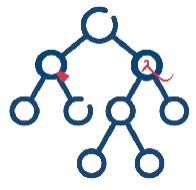
\includegraphics[height=1.0cm]{msca_logo.png}}%
    \end{center}

    \vspace{0.6cm}

    % Main title with Q logos on sides (with clickable links)
    \begin{center}
        \begin{minipage}{0.1\textwidth}
            \centering
            \href{https://quantlet.com}{
\includegraphics[height=1.1cm]{ql_logo.png}}
        \end{minipage}%
        \begin{minipage}{0.78\textwidth}
            \centering
            {\LARGE\bfseries\usebeamercolor[fg]{title}\inserttitle}

            \vspace{0.3cm}

            {\usebeamerfont{subtitle}\usebeamercolor[fg]{title}\insertsubtitle}
        \end{minipage}%
        \begin{minipage}{0.1\textwidth}
            \centering
            \href{https://quantinar.com}{
\includegraphics[height=1.1cm]{qr_logo.png}}
        \end{minipage}
    \end{center}

    \vspace{0.6cm}

    % Authors (left aligned)
    \hspace{0.5cm}{\usebeamerfont{author}\insertauthor}

    \vspace{0.3cm}

    % Institute/Affiliations (left aligned)
    \hspace{0.5cm}\begin{minipage}[t]{0.9\textwidth}
        \raggedright\small\insertinstitute
    \end{minipage}
}

%=============================================================================
% THEOREM ENVIRONMENTS
%=============================================================================
\theoremstyle{definition}
\setbeamertemplate{theorems}[numbered]
\ifdefined\atslang
\newtheorem{defn}{Definiție}
\newtheorem{thm}{Teoremă}
\newtheorem{prop}{Propoziție}
\newtheorem{rmk}{Observație}
\else
\newtheorem{defn}{Definition}
\newtheorem{thm}{Theorem}
\newtheorem{prop}{Proposition}
\newtheorem{rmk}{Remark}
\fi

%=============================================================================
% CENTRED MINIPAGE (no extra vertical space)
%=============================================================================
\newenvironment{cminipage}[1]{%
    \par\noindent\hfill\begin{minipage}{#1}\ignorespaces
}{%
    \end{minipage}\hfill\null\par
}

%=============================================================================
% CUSTOM COMMANDS
%=============================================================================
\newcommand{\E}{\mathbb{E}}
\newcommand{\Var}{\text{Var}}
\newcommand{\Cov}{\text{Cov}}
\newcommand{\Corr}{\text{Corr}}
\newcommand{\R}{\mathbb{R}}
\newcommand{\N}{\mathbb{N}}
\newcommand{\Z}{\mathbb{Z}}
\newcommand{\B}{\mathbf{B}}
\newcommand{\imark}{\textcolor{MainBlue}{\textbullet}}
\newcommand{\RMSE}{\text{RMSE}}
\newcommand{\MAE}{\text{MAE}}
\newcommand{\MAPE}{\text{MAPE}}

% Boldface vector/matrix commands (VAR, VECM, state space)
\newcommand{\bY}{\mathbf{Y}}
\newcommand{\bX}{\mathbf{X}}
\newcommand{\bA}{\mathbf{A}}
\newcommand{\bB}{\mathbf{B}}
\newcommand{\bepsilon}{\boldsymbol{\varepsilon}}
\newcommand{\bSigma}{\boldsymbol{\Sigma}}
\newcommand{\bPhi}{\boldsymbol{\Phi}}
\newcommand{\bGamma}{\boldsymbol{\Gamma}}
\newcommand{\bPi}{\boldsymbol{\Pi}}
\newcommand{\bc}{\mathbf{c}}
\newcommand{\balpha}{\boldsymbol{\alpha}}
\newcommand{\bbeta}{\boldsymbol{\beta}}
\newcommand{\bvarepsilon}{\boldsymbol{\varepsilon}}

% Seminar marks
\newcommand{\correct}{\textcolor{Forest}{\checkmark}}
\newcommand{\incorrect}{\textcolor{Crimson}{\texttimes}}


\newcommand{\qlurl}[1]{https://github.com/danpele/Advanced-Time-Series/tree/main/Quantlets/Ch_13/#1}

% Clickable citations (DOIs verified via Crossref)
\newcommand{\refAks}{\href{https://arxiv.org/abs/2410.10393}{Aksu et al.\ (2024)}}
\newcommand{\refAns}{\href{https://arxiv.org/abs/2403.07815}{Ansari et al.\ (2024)}}
\newcommand{\refAnsB}{\href{https://arxiv.org/abs/2510.15821}{Ansari et al.\ (2025)}}
\newcommand{\refAue}{\href{https://arxiv.org/abs/2505.23719}{Auer et al.\ (2025)}}
\newcommand{\refBom}{\href{https://arxiv.org/abs/2108.07258}{Bommasani et al.\ (2021)}}
\newcommand{\refBri}{\href{https://arxiv.org/abs/2607.05291}{Brini (2026)}}
\newcommand{\refCoh}{\href{https://arxiv.org/abs/2505.14766}{Cohen et al.\ (2025)}}
\newcommand{\refDas}{\href{https://arxiv.org/abs/2310.10688}{Das et al.\ (2024)}}
\newcommand{\refEdw}{\href{https://arxiv.org/abs/2405.13867}{Edwards et al.\ (2024)}}
\newcommand{\refGar}{\href{https://arxiv.org/abs/2310.03589}{Garza et al.\ (2023)}}
\newcommand{\refGarB}{\href{https://arxiv.org/abs/2603.08707}{Garza et al.\ (2026)}}
\newcommand{\refGoe}{\href{https://arxiv.org/abs/2505.11163}{Goel et al.\ (2025)}}
\newcommand{\refGos}{\href{https://arxiv.org/abs/2402.03885}{Goswami et al.\ (2024)}}
\newcommand{\refGru}{\href{https://arxiv.org/abs/2310.07820}{Gruver et al.\ (2023)}}
\newcommand{\refHof}{\href{https://arxiv.org/abs/2203.15556}{Hoffmann et al.\ (2022)}}
\newcommand{\refJin}{\href{https://arxiv.org/abs/2310.01728}{Jin et al.\ (2024)}}
\newcommand{\refKap}{\href{https://arxiv.org/abs/2001.08361}{Kaplan et al.\ (2020)}}
\newcommand{\refLiu}{\href{https://arxiv.org/abs/2511.11698}{Liu et al.\ (2025)}}
\newcommand{\refLTZ}{\href{https://arxiv.org/abs/2504.14765}{Lopez-Lira, Tang and Zhu (2025)}}
\newcommand{\refMey}{\href{https://arxiv.org/abs/2512.20761}{Meyer et al.\ (2025)}}
\newcommand{\refNie}{\href{https://arxiv.org/abs/2211.14730}{Nie et al.\ (2023)}}
\newcommand{\refPE}{\href{https://arxiv.org/abs/2607.02623}{Pan and Ezzat (2026)}}
\newcommand{\refRas}{\href{https://arxiv.org/abs/2310.08278}{Rasul et al.\ (2023)}}
\newcommand{\refRNW}{\href{https://arxiv.org/abs/2511.18578}{Rahimikia, Ni and Wang (2025)}}
\newcommand{\refShc}{\href{https://arxiv.org/abs/2509.26468}{Shchur et al.\ (2025)}}
\newcommand{\refShi}{\href{https://arxiv.org/abs/2405.15124}{Shi et al.\ (2024)}}
\newcommand{\refTan}{\href{https://arxiv.org/abs/2406.16964}{Tan et al.\ (2024)}}
\newcommand{\refVas}{\href{https://arxiv.org/abs/1706.03762}{Vaswani et al.\ (2017)}}
\newcommand{\refWoo}{\href{https://arxiv.org/abs/2402.02592}{Woo et al.\ (2024)}}
\newcommand{\refYao}{\href{https://arxiv.org/abs/2410.12360}{Yao et al.\ (2025)}}
\newcommand{\refZho}{\href{https://arxiv.org/abs/2302.11939}{Zhou et al.\ (2023)}}
\newcommand{\refBH}{\href{https://doi.org/10.1111/j.2517-6161.1995.tb02031.x}{Benjamini and Hochberg (1995)}}
\newcommand{\refBol}{\href{https://doi.org/10.1016/0304-4076(86)90063-1}{Bollerslev (1986)}}
\newcommand{\refChr}{\href{https://doi.org/10.2307/2527341}{Christoffersen (1998)}}
\newcommand{\refCor}{\href{https://doi.org/10.1093/jjfinec/nbp001}{Corsi (2009)}}
\newcommand{\refDem}{\href{https://jmlr.org/papers/v7/demsar06a.html}{Demšar (2006)}}
\newcommand{\refDM}{\href{https://doi.org/10.1080/07350015.1995.10524599}{Diebold and Mariano (1995)}}
\newcommand{\refEM}{\href{https://doi.org/10.1198/073500104000000370}{Engle and Manganelli (2004)}}
\newcommand{\refFW}{\href{https://doi.org/10.1145/5666.5673}{Fleming and Wallace (1986)}}
\newcommand{\refGR}{\href{https://doi.org/10.1198/016214506000001437}{Gneiting and Raftery (2007)}}
\newcommand{\refGW}{\href{https://doi.org/10.1111/j.1468-0262.2006.00718.x}{Giacomini and White (2006)}}
\newcommand{\refHAB}{\href{https://doi.org/10.1007/s10618-022-00894-5}{Hewamalage, Ackermann and Bergmeir (2023)}}
\newcommand{\refHLN}{\href{https://doi.org/10.1016/S0169-2070(96)00719-4}{Harvey, Leybourne and Newbold (1997)}}
\newcommand{\refHLNa}{\href{https://doi.org/10.3982/ECTA5771}{Hansen, Lunde and Nason (2011)}}
\newcommand{\refHF}{\href{https://doi.org/10.1016/j.ijforecast.2015.11.011}{Hong and Fan (2016)}}
\newcommand{\refHK}{\href{https://doi.org/10.1016/j.ijforecast.2006.03.001}{Hyndman and Koehler (2006)}}
\newcommand{\refHKSG}{\href{https://doi.org/10.1016/S0169-2070(01)00110-8}{Hyndman et al.\ (2002)}}
\newcommand{\refHol}{\href{https://www.jstor.org/stable/4615733}{Holm (1979)}}
\newcommand{\refKup}{\href{https://doi.org/10.3905/jod.1995.407942}{Kupiec (1995)}}
\newcommand{\refLim}{\href{https://doi.org/10.1016/j.ijforecast.2021.03.012}{Lim et al.\ (2021)}}
\newcommand{\refMak}{\href{https://doi.org/10.1016/j.ijforecast.2021.11.013}{Makridakis, Spiliotis and Assimakopoulos (2022)}}
\newcommand{\refOMI}{\href{https://web.archive.org/web/20220301022212/https://realized.oxford-man.ox.ac.uk/}{Heber et al.\ (2009)}}
\newcommand{\refOre}{\href{https://arxiv.org/abs/1905.10437}{Oreshkin et al.\ (2020)}}
\newcommand{\refPat}{\href{https://doi.org/10.1016/j.jeconom.2010.03.034}{Patton (2011)}}
\newcommand{\refPet}{\href{https://doi.org/10.1016/j.ijforecast.2021.11.001}{Petropoulos et al.\ (2022)}}
\newcommand{\refSal}{\href{https://doi.org/10.1016/j.ijforecast.2019.07.001}{Salinas et al.\ (2020)}}
\newcommand{\refZen}{\href{https://doi.org/10.1609/aaai.v37i9.26317}{Zeng et al.\ (2023)}}
\newcommand{\refZW}{\href{https://doi.org/10.1016/j.eneco.2017.12.016}{Ziel and Weron (2018)}}
\newcommand{\refAB}{\href{https://doi.org/10.1561/2200000101}{Angelopoulos and Bates (2023)}}
\newcommand{\refACT}{\href{https://arxiv.org/abs/2307.16895}{Angelopoulos, Candès and Tibshirani (2023)}}
\newcommand{\refBar}{\href{https://doi.org/10.1214/23-AOS2276}{Barber et al.\ (2023)}}
\newcommand{\refBarB}{\href{https://doi.org/10.1093/imaiai/iaaa017}{Foygel Barber et al.\ (2021)}}
\newcommand{\refCWZ}{\href{https://arxiv.org/abs/1802.06300}{Chernozhukov, Wüthrich and Zhu (2018)}}
\newcommand{\refGC}{\href{https://arxiv.org/abs/2106.00170}{Gibbs and Candès (2021)}}
\newcommand{\refGCb}{\href{https://jmlr.org/papers/v25/22-1218.html}{Gibbs and Candès (2024)}}
\newcommand{\refKB}{\href{https://doi.org/10.2307/1913643}{Koenker and Bassett (1978)}}
\newcommand{\refLei}{\href{https://doi.org/10.1080/01621459.2017.1307116}{Lei et al.\ (2018)}}
\newcommand{\refLW}{\href{https://doi.org/10.1111/rssb.12021}{Lei and Wasserman (2014)}}
\newcommand{\refOli}{\href{https://arxiv.org/abs/2203.15885}{Oliveira et al.\ (2024)}}
\newcommand{\refPap}{\href{https://doi.org/10.1007/3-540-36755-1_29}{Papadopoulos et al.\ (2002)}}
\newcommand{\refRPC}{\href{https://arxiv.org/abs/1905.03222}{Romano, Patterson and Candès (2019)}}
\newcommand{\refTBCR}{\href{https://arxiv.org/abs/1904.06019}{Tibshirani et al.\ (2019)}}
\newcommand{\refVGS}{\href{https://doi.org/10.1007/b106715}{Vovk, Gammerman and Shafer (2005)}}
\newcommand{\refVGSb}{\href{https://doi.org/10.1007/978-3-031-06649-8}{Vovk, Gammerman and Shafer (2022)}}
\newcommand{\refVov}{\href{https://proceedings.mlr.press/v25/vovk12.html}{Vovk (2012)}}
\newcommand{\refWin}{\href{https://doi.org/10.1080/01621459.1972.10481224}{Winkler (1972)}}
\newcommand{\refXX}{\href{https://proceedings.mlr.press/v139/xu21h.html}{Xu and Xie (2021)}}
\newcommand{\refXXb}{\href{https://doi.org/10.1109/TPAMI.2023.3272339}{Xu and Xie (2023)}}
\newcommand{\refZaf}{\href{https://arxiv.org/abs/2202.07282}{Zaffran et al.\ (2022)}}
\newcommand{\refCO}{\href{https://github.com/danpele/Conformal_Oracle}{Pele et al.\ (Conformal\_Oracle)}}
\newcommand{\refTV}{\href{https://github.com/danpele/TSFM_VaR_CEE}{Pele et al.\ (TSFM\_VaR\_CEE)}}

\title[Advanced Time Series Analysis and Forecasting]{Advanced Time Series Analysis and Forecasting}
\subtitle{Chapter 13: Foundation models and conformal prediction}
\author[D.T. Pele]{Daniel Traian PELE}
\institute{Bucharest University of Economic Studies\\
IDA Institute Digital Assets\\
Blockchain Research Center\\
AI4EFin Artificial Intelligence for Energy Finance\\
Romanian Academy, Institute for Economic Forecasting\\
MSCA Digital Finance}
\date{}

%=============================================================================
\providecommand{\atsapplink}[3]{\hypertarget{#2}{}\hyperlink{#1}{\beamergotobutton{#3}}}  % APPLINKS-MACROS
\providecommand{\atsappback}[2]{\begin{tikzpicture}[remember picture,overlay]\node[anchor=south east] at ([xshift=-3mm,yshift=7mm]current page.south east){\hyperlink{#1}{\beamerreturnbutton{#2}}};\end{tikzpicture}}  % APPLINKS-MACROS
\providecommand{\atschlink}[2]{\href{#1}{#2}}  % APPLINKS-MACROS
\providecommand{\atschlinkt}[2]{\href{#1}{\usebeamercolor[fg]{frametitle}#2}}  % APPLINKS-MACROS
\begin{document}
%=============================================================================

{
\setbeamertemplate{headline}{}
\setbeamertemplate{footline}{}
\begin{frame}[noframenumbering]
    \titlepage
\end{frame}
}
% BEGIN-ACRONYMS (generat de latex/acronyms.py; nu editati manual)
\begin{frame}{Acronyms used in this material (1/2)}
\setbeamertemplate{itemize/enumerate body begin}{\tiny}
\begin{columns}[T]
\begin{column}{0.49\textwidth}
\begin{itemize}\setlength{\itemsep}{0pt}
    \item \textbf{ACI}: Adaptive Conformal Inference
    \item \textbf{AI}: Artificial Intelligence
    \item \textbf{AIC}: Akaike Information Criterion
    \item \textbf{API}: Application Programming Interface
    \item \textbf{AR}: AutoRegressive (model); in event studies: Abnormal Return
    \item \textbf{ARX}: AutoRegressive model with eXogenous variables
    \item \textbf{BET}: Bucharest Exchange Trading (index)
    \item \textbf{BH}: Benjamini–Hochberg (procedure)
    \item \textbf{BOOM}: Benchmark Of Observability Metrics
    \item \textbf{CEE}: Central and Eastern Europe
    \item \textbf{CPM}: Contiguous Patch Masking
    \item \textbf{CPU}: Central Processing Unit
    \item \textbf{CQR}: Conformalized Quantile Regression
\end{itemize}
\end{column}
\begin{column}{0.49\textwidth}
\begin{itemize}\setlength{\itemsep}{0pt}
    \item \textbf{CRPS}: Continuous Ranked Probability Score
    \item \textbf{DM}: Diebold–Mariano (test)
    \item \textbf{DQ}: Dynamic Quantile (test of Engle and Manganelli)
    \item \textbf{ENTSO-E}: European Network of Transmission System Operators for Electricity
    \item \textbf{EODHD}: EOD Historical Data (market-data provider)
    \item \textbf{ETS}: Error, Trend, Seasonality (exponential smoothing state space models)
    \item \textbf{EU}: European Union
    \item \textbf{FDR}: False Discovery Rate
    \item \textbf{FWER}: Family-Wise Error Rate
    \item \textbf{GARCH}: Generalised AutoRegressive Conditional Heteroskedasticity
    \item \textbf{GIFT}: General Time Series Forecasting Model Evaluation (the GIFT-Eval benchmark)
    \item \textbf{GPT-2}: Generative Pre-trained Transformer 2 (OpenAI language model)
    \item \textbf{GPT4TS}: GPT for Time Series (One Fits All)
\end{itemize}
\end{column}
\end{columns}
\end{frame}
\begin{frame}{Acronyms used in this material (2/2)}
\setbeamertemplate{itemize/enumerate body begin}{\tiny}
\begin{columns}[T]
\begin{column}{0.49\textwidth}
\begin{itemize}\setlength{\itemsep}{0pt}
    \item \textbf{GW}: Giacomini–White (test of conditional predictive ability)
    \item \textbf{HAC}: Heteroskedasticity and Autocorrelation Consistent (standard errors)
    \item \textbf{HAR}: Heterogeneous AutoRegressive (model)
    \item \textbf{HICP}: Harmonised Index of Consumer Prices
    \item \textbf{HLN}: Harvey–Leybourne–Newbold (small-sample correction of the DM test)
    \item \textbf{ID}: Identifier (arXiv or DOI)
    \item \textbf{LLM}: Large Language Model
    \item \textbf{LOTSA}: Large-scale Open Time Series Archive
    \item \textbf{MAE}: Mean Absolute Error
    \item \textbf{MASE}: Mean Absolute Scaled Error
    \item \textbf{MCS}: Model Confidence Set
    \item \textbf{MOMENT}: MOMENT, a family of open time-series foundation models
    \item \textbf{MSE}: Mean Squared Error
\end{itemize}
\end{column}
\begin{column}{0.49\textwidth}
\begin{itemize}\setlength{\itemsep}{0pt}
    \item \textbf{NVIDIA}: NVIDIA Corporation (graphics processors)
    \item \textbf{OOD}: Out Of Distribution
    \item \textbf{PID}: Proportional--Integral--Derivative (controller)
    \item \textbf{QLIKE}: Quasi-LIKElihood loss
    \item \textbf{RLHF}: Reinforcement Learning from Human Feedback
    \item \textbf{RV}: Realised Variance
    \item \textbf{TS}: Time Series (in TS-Arena)
    \item \textbf{TSA}: Time Series Analysis
    \item \textbf{VAT}: Value Added Tax
    \item \textbf{WQL}: Weighted Quantile Loss
\end{itemize}
\end{column}
\end{columns}
\end{frame}
% END-ACRONYMS

\begin{frame}{Today's question and route}
\itemsize{\small}
\begin{itemize}
    \item \textbf{Question}: can one pretrained model forecast series it has never seen, and how do we turn any forecast, pretrained or not, into intervals whose coverage we can guarantee or at least control?
    \begin{itemize}
        \item two halves of one problem: point and quantile accuracy (foundation models), then honest uncertainty (conformal prediction)
    \end{itemize}
    \item \textbf{Route} of the chapter
    \begin{itemize}
        \item pretraining: data, tokens, patches, scaling laws; model families and design choices
        \item benchmarks, contamination and testing across many series; evidence on Romanian and EU data; LLMs and their critique
        \item conformal prediction: exchangeability, split conformal, CQR, the limits of conditional coverage
        \item dependent data: weights, EnbPI, ACI, conformal PID; diagnostics; calibrating foundation-model intervals and VaR
    \end{itemize}
    \item We build on \atschlink{https://danpele.github.io/Time-Series-Analysis/EN/Courses/chapter11_foundation_models_time_series.pdf}{TSA, Chapter 11} (Chronos, TimesFM, Moirai, zero-shot tests, CRPS and WQL), on \atschlink{https://danpele.github.io/Advanced-Time-Series/EN/Courses/chapter1_forecast_evaluation.pdf}{Chapter 1} (scoring rules, DM, MCS), \atschlink{https://danpele.github.io/Advanced-Time-Series/EN/Courses/chapter9_var_es_backtesting.pdf}{Chapter 9} (VaR backtests, ACI for VaR) and \atschlink{https://danpele.github.io/Advanced-Time-Series/EN/Courses/chapter12_machine_learning_deep_learning.pdf}{Chapter 12} (deep architectures); Seminar 13 comes before this lecture
\end{itemize}
\end{frame}

\begin{frame}{Learning outcomes}
\itemsize{\small}
\begin{itemize}
    \item Explain how a time series foundation model is pretrained: corpus, scaling, tokenisation or patching, output head and loss
    \item Compare model families and choose between zero-shot use, fine-tuning and in-context covariates
    \item Design a benchmark without leakage or contamination and test differences across many series with corrections for multiplicity
    \item Prove the coverage of split conformal and CQR, and state what conformal prediction cannot guarantee
    \item Apply weighted conformal, EnbPI, ACI and conformal PID to dependent data, diagnose coverage and calibrate foundation-model intervals
\end{itemize}
\end{frame}

\begin{frame}{Reading, data and tools}
\itemsize{\small}
\begin{itemize}
    \item Foundation models: \refAns; \refAnsB; \refDas; \refWoo; \refAue; benchmarks: \refAks; \refShc
    \begin{itemize}
        \item Conformal prediction: \refVGSb; \refAB; \refRPC; \refBar; \refGC; \refACT; \refXX
        \item Critique and evaluation: \refTan; \refHAB; survey of forecasting practice: \refPet
    \end{itemize}
    \item Python Quantlets of this chapter: \href{https://github.com/danpele/Advanced-Time-Series/tree/main/Quantlets/Ch_13}{Quantlets/Ch\_13}
    \begin{itemize}
        \item open checkpoints on a CPU: \texttt{chronos-forecasting} (Chronos-Bolt, Chronos-2), \texttt{timesfm} (TimesFM 2.5), \texttt{tirex-ts} (TiRex); conformal methods, DM, MCS and backtests written in \texttt{numpy}
    \end{itemize}
    \item Lecture notebook: \href{\colaburl{notebooks/EN/chapter13_lecture_notebook.ipynb}}{open in Google Colab}
\end{itemize}
\end{frame}

\begin{frame}{Data used in this chapter}
\itemsize{\footnotesize}
\begin{center}
\scriptsize
\begin{tabular}{>{\raggedright\arraybackslash}p{3.9cm}>{\raggedright\arraybackslash}p{5.3cm}>{\raggedright\arraybackslash}p{2.9cm}}
\toprule
\textbf{Series} & \textbf{Source} & \textbf{Sample} \\
\midrule
Romanian electricity load, hourly & Energy-Charts (ENTSO-E transparency data) & 2022 -- 30 September 2026 \\
Bucharest air temperature, hourly & Open-Meteo historical archive & 2022 -- 2026 \\
HICP annual inflation, 27 EU countries & Eurostat, monthly & 2000 -- August 2026 \\
Realised variance, 5-minute returns & Bitcoin: Binance; S\&P 500: Oxford-Man \refOMI{} & 2018 -- 2026; 2000 -- 2022 \\
BET, S\&P 500, NVIDIA, daily & EODHD daily closes & 2000 -- 2026 \\
\bottomrule
\end{tabular}
\end{center}
\begin{itemize}
    \item Returns are 100 times log differences; the realised variance is in squared percent; every forecast uses only data available at its origin
\end{itemize}
\end{frame}

\begin{frame}{Two lines of research that met}
\itemsize{\footnotesize}
\begin{columns}[T]
\begin{column}{0.4\textwidth}
\centering
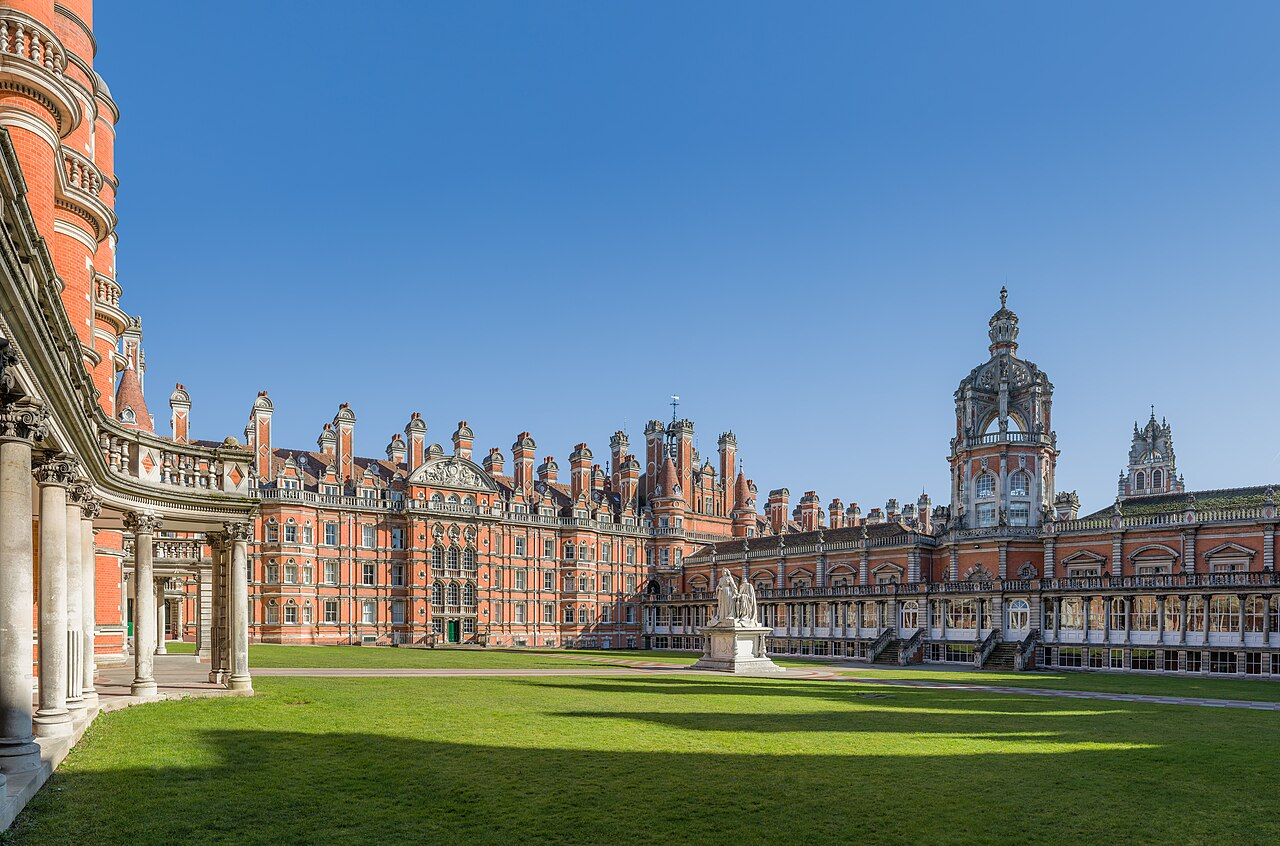
\includegraphics[height=0.36\textheight]{ch13_royal_holloway.jpg}\\[1mm]
\imgcap{Royal Holloway, University of London: the Founder's Building}
\imgcredit{https://commons.wikimedia.org/wiki/File:Founder's_Building,_Royal_Holloway,_University_of_London_-_Diliff.jpg}{Photo: Diliff (2015); CC BY-SA 3.0; Wikimedia Commons}
\end{column}
\begin{column}{0.58\textwidth}
\begin{itemize}
    \item 1990s--2005: conformal prediction at Royal Holloway: Vovk, Gammerman and Shafer, rooted in Kolmogorov's algorithmic randomness \refVGS
    \item 2002--2018: split (inductive) conformal \refPap; distribution-free regression \refLei; 2019: CQR \refRPC
    \item 2021--2023: time series: ACI \refGC, EnbPI \refXX, conformal PID \refACT, beyond exchangeability \refBar
    \item 2017--2025: Transformers \refVas, foundation models \refBom; for series: Lag-Llama, TimesFM, Moirai, Chronos (2023--2024), TiRex, Chronos-2 (2025)
\end{itemize}
\end{column}
\end{columns}
\end{frame}

\begin{frame}{Known from TSA and new here}
\itemsize{\small}
\begin{itemize}
    \item Known (\atschlink{https://danpele.github.io/Time-Series-Analysis/EN/Courses/chapter11_foundation_models_time_series.pdf}{TSA, Chapter 11}): zero-shot use of Chronos, TimesFM, Moirai and Lag-Llama; mean scaling and quantisation in brief; pinball loss, CRPS, WQL, MASE; first warnings about contamination
    \item New: the research toolkit
    \begin{itemize}
        \item design choices and their consequences (range limits, quantile heads, patching, covariates in context), scaling evidence
        \item benchmarks with pre-registered windows after the model releases, tests across many series with Holm and BH corrections
        \item conformal theory with proofs, its failure under dependence and the online methods that repair it, with coverage diagnostics
    \end{itemize}
    \item Case studies: Ansari et al.\ (2024), Tan et al.\ (2024), Romano--Patterson--Candès (2019), Gibbs--Candès (2021), Barber et al.\ (2023), Angelopoulos--Candès--Tibshirani (2023), Xu--Xie (2021), with the designs of the papers, on our data
\end{itemize}
\end{frame}


%=============================================================================
\section{Pretraining for time series}
%=============================================================================

\begin{frame}{A foundation model as an amortised forecaster}
\itemsize{\small}
\begin{itemize}
    \item \textbf{Pretraining}: $\hat\theta = \arg\min_\theta \sum_{s \in \mathcal D_{\mathrm{pre}}}\sum_t \ell\big(y^{(s)}_{t+1:t+H}, f_\theta(y^{(s)}_{t-C+1:t})\big)$ over a corpus $\mathcal D_{\mathrm{pre}}$ of many series
    \begin{itemize}
        \item $C$: context length; $H$: horizon; $\ell$: a scoring rule (cross-entropy, pinball, negative log-likelihood)
        \item the term \textbf{foundation model} \refBom: trained once on broad data, then adapted to many tasks
    \end{itemize}
    \item \textbf{Zero-shot} use: $\hat\theta$ fixed, the forecast for a new series is $f_{\hat\theta}(y_{T-C+1:T})$; no parameter is estimated on the target
    \begin{itemize}
        \item the network performs the estimation step inside its forward pass: inference is amortised over the corpus
    \end{itemize}
    \item A global model of \atschlink{https://danpele.github.io/Advanced-Time-Series/EN/Courses/chapter12_machine_learning_deep_learning.pdf}{Chapter 12} is trained on the series of one data set; a foundation model on many data sets, frequencies and domains
\end{itemize}
\end{frame}

\begin{frame}{Structure shared across series}
\itemsize{\small}
\begin{itemize}
    \item Shapes recur across domains: seasonal profiles, damped trends, level shifts, volatility clusters, intermittency
    \begin{itemize}
        \item after scaling, a load curve and a web-traffic curve can look alike: the model learns a prior over shapes
    \end{itemize}
    \item Not shared: the economics of a particular series (a tax change, a policy rule, a holiday calendar)
    \begin{itemize}
        \item unless it is passed as a covariate in the context (Chronos-2) or learned by fine-tuning
    \end{itemize}
    \item A no-free-lunch caveat: averaged over all processes no forecaster wins; pretraining helps only if the target resembles the corpus
    \begin{itemize}
        \item financial returns are close to a martingale difference: little shape to transfer, much to overfit
    \end{itemize}
\end{itemize}
\end{frame}

\begin{frame}{Pretraining data: scale and composition}
\itemsize{\small}
\begin{itemize}
    \item Chronos \refAns: public data sets plus two augmentations: \textbf{TSMixup} (convex mixtures of real series) and \textbf{KernelSynth} (series drawn from Gaussian processes with random composite kernels)
    \item TimesFM \refDas: about $10^{11}$ time points: Google Trends, Wikipedia page views, synthetic and public series; Moirai \refWoo: LOTSA, over 27 billion observations in nine domains
    \item Toto \refCoh: observability metrics of a cloud provider, a corpus 4--10 times larger than those of earlier models; GIFT-Eval \refAks: a \textbf{non-leaking} pretraining set of about 230 billion points
    \item Composition matters more than size for us: economic and financial series are a small, low-frequency share of every corpus
\end{itemize}
\end{frame}

\begin{frame}{Tokenisation: from real values to a vocabulary}
\itemsize{\small}
\begin{itemize}
    \item Chronos \refAns: \textbf{mean scaling} $\tilde x_t = x_t/s$, $s = \frac1C\sum_{t \le C}|x_t|$ (context only), then \textbf{uniform bins} on $[-15, 15]$; 4096 tokens including special ones
    \begin{itemize}
        \item the model is a language model (T5) trained with \textbf{cross-entropy}: the forecast is a categorical distribution over bins, sampled autoregressively
        \item no notion of distance between tokens: neighbouring bins are as different as distant ones, unless the data teach otherwise
    \end{itemize}
    \item Consequences: resolution $30s/4092$; values above $15s$ cannot be predicted; scale-invariant by construction
    \item LLMTime \refGru: digits as text tokens; Lag-Llama \refRas: lagged values as features; patch models: no vocabulary at all
\end{itemize}
\end{frame}

\begin{frame}{The Chronos tokeniser on real data}
\itemsize{\footnotesize}
\begin{center}
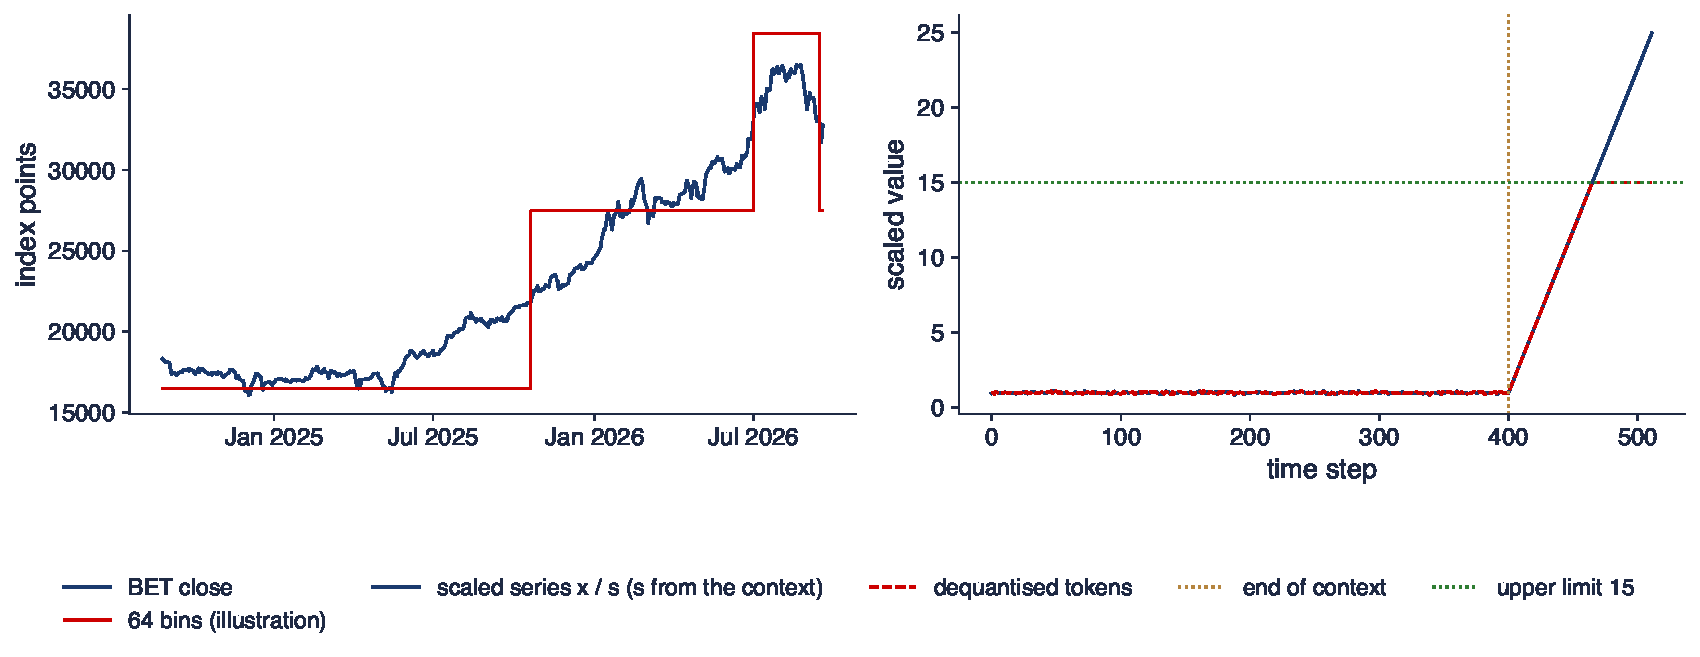
\includegraphics[width=0.97\textwidth,height=0.5\textheight,keepaspectratio]{ats_ch13_tokens.pdf}
\end{center}
\vspace{-0.25cm}
\begin{itemize}
    \item Left: BET closes, 27 August 2024 -- 18 September 2026 ($C = 512$), and a 64-bin quantisation (illustration); right: a context near 1 followed by a rise to 25 times that level
\end{itemize}
\quantlet{ATS\_ch13\_pretraining}{\qlurl{ATS_ch13_pretraining}}
\end{frame}

\begin{frame}{Interpreting the tokeniser}
\itemsize{\small}
\begin{itemize}
    \item BET: $s = 23\,072$ points, bin width 169.1 points, maximum quantisation error 84.5 points: negligible for prices, but a fixed share of the level
    \item Right panel: the scale is set by the context, so the path that rises beyond $15s$ is clipped: 42\% of the future steps are unreachable, the last one by 40\%
    \item Explosive series (bubbles, \atschlink{https://danpele.github.io/Advanced-Time-Series/EN/Courses/chapter16_explosive_roots_bubbles.pdf}{Chapter 16}; hyperinflation) are outside the support of a mean-scaled vocabulary; Chronos-2 replaces it by an arcsinh transform and quantile outputs
\end{itemize}
\end{frame}

\begin{frame}{Patching and the output head}
\itemsize{\small}
\begin{itemize}
    \item \textbf{Patching} \refNie: split the context into patches of $P$ consecutive values, embed each patch as one token; attention costs $O((C/P)^2)$ instead of $O(C^2)$
    \begin{itemize}
        \item TimesFM \refDas: input patches of 32, output patches of 128 (fewer autoregressive steps); Chronos-Bolt and Chronos-2: patches of 16; Moirai \refWoo: several patch sizes by frequency
    \end{itemize}
    \item Output heads
    \begin{itemize}
        \item categorical over bins (Chronos); \textbf{quantile head} trained by the pinball loss (Chronos-Bolt: 10\%--90\%; Chronos-2: 1\%--99\%; TimesFM 2.5, TiRex: deciles)
        \item parametric: Student-$t$ (Lag-Llama \refRas), a mixture of distributions (Moirai)
    \end{itemize}
    \item Direct multi-step quantiles (one pass for $H$ steps) avoid error accumulation but give marginal, not joint, predictive distributions: path functionals (a maximum, a sum) need care
\end{itemize}
\end{frame}

\begin{frame}{Scaling laws}
\itemsize{\small}
\begin{itemize}
    \item Language models \refKap, \refHof: test loss falls as a power law, $L(N) \approx (N_c/N)^{\alpha_N}$, in the number of parameters $N$, data and compute, over orders of magnitude
    \item Time series: decoder-only Transformers show the same power laws in parameters, data and compute \refEdw; the look-back length interacts with data size \refShi
    \begin{itemize}
        \item out-of-distribution: the log-likelihood scales similarly in and out of distribution, but architecture matters; tweaks that help in distribution can reduce OOD scalability \refYao
    \end{itemize}
    \item A scaling law is a statement about average loss on the corpus distribution, not about one Romanian series; small models (TiRex, 35 million parameters) beat larger ones on public leaderboards \refAue
\end{itemize}
\end{frame}

\begin{frame}{Size and accuracy on our three tasks}
\itemsize{\footnotesize}
\begin{center}
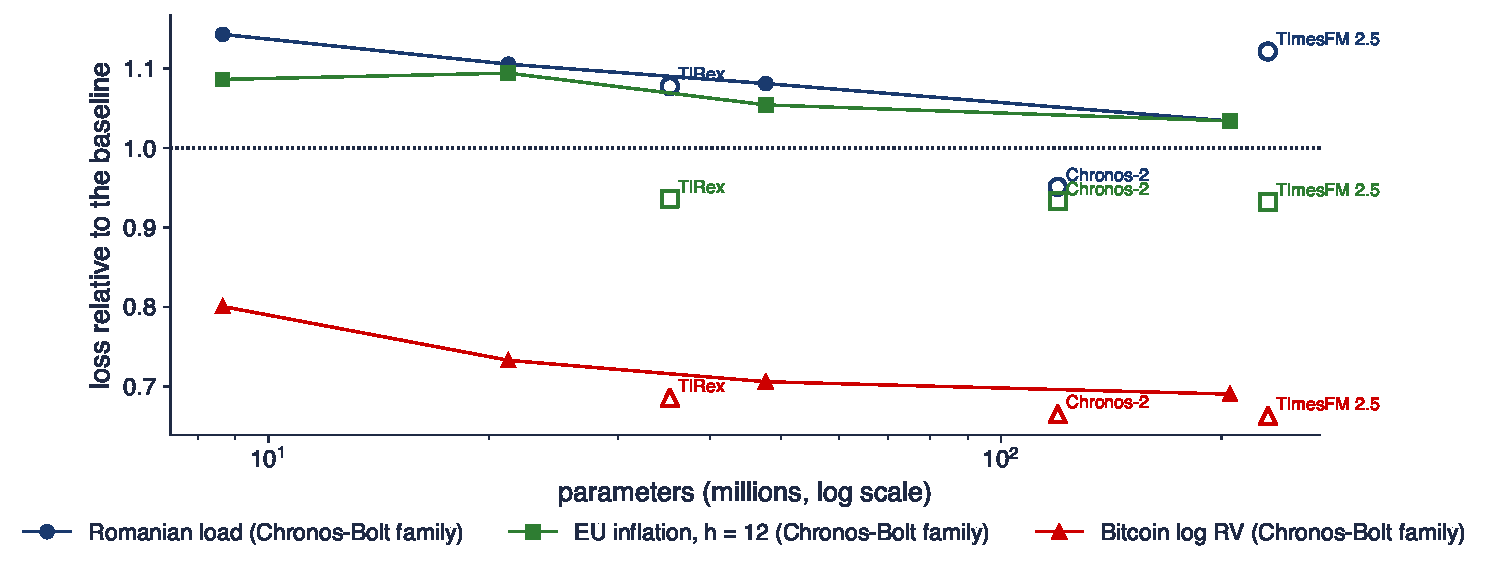
\includegraphics[width=0.97\textwidth,height=0.5\textheight,keepaspectratio]{ats_ch13_scaling.pdf}
\end{center}
\vspace{-0.25cm}
\begin{itemize}
    \item Losses relative to the task baseline: Romanian load (MAE / expert ARX, 2025--2026), EU inflation (MAE / random walk, $h = 12$, geometric mean over 27 countries), Bitcoin log RV (MSE / HAR); parameters counted in the loaded checkpoints
\end{itemize}
\quantlet{ATS\_ch13\_pretraining}{\qlurl{ATS_ch13_pretraining}}
\end{frame}

\begin{frame}{Interpreting size against accuracy}
\itemsize{\small}
\begin{itemize}
    \item Chronos-Bolt family (9--205 M parameters): load 1.143 $\to$ 1.034, inflation 1.086 $\to$ 1.034, Bitcoin 0.800 $\to$ 0.690
    \item Across families size is not the ranking: Chronos-2 (119 M) 0.951 on load; TiRex (35 M) 1.078; TimesFM 2.5 (231 M) 1.121
    \item Within the Chronos-Bolt family the loss falls with size on all three tasks (one exception: mini on inflation); across families architecture, corpus and training recipe change together, so three tasks are not a scaling study
\end{itemize}
\end{frame}

\begin{frame}{Recap: pretraining}
\itemsize{\small}
\begin{itemize}
    \item Pretraining amortises estimation over a corpus; zero-shot use runs the estimator inside one forward pass
    \item Mean scaling and binning give scale invariance but a hard range; patching and quantile heads trade it for direct multi-step quantiles
    \item Scaling laws hold on average over corpora; on a given economic series, design and data matter more than size
\end{itemize}
\end{frame}


%=============================================================================
\section{Model families and design choices}
%=============================================================================

\begin{frame}{The main open models}
\itemsize{\footnotesize}
\begin{center}
\scriptsize
\begin{tabular}{>{\raggedright\arraybackslash}p{2.2cm}>{\raggedright\arraybackslash}p{3.4cm}>{\raggedright\arraybackslash}p{2.0cm}>{\raggedright\arraybackslash}p{3.9cm}}
\toprule
\textbf{Model} & \textbf{Architecture} & \textbf{Parameters} & \textbf{Output} \\
\midrule
Chronos \refAns{} & T5 encoder--decoder on tokens & 20--710 M & categorical, sampled paths \\
Chronos-Bolt & T5 on patches of 16 & 9--205 M & 9 quantiles, 10\%--90\%, 64 steps \\
Chronos-2 \refAnsB{} & encoder with group attention & 119 M & 21 quantiles, 1\%--99\%; covariates \\
TimesFM 2.5 \refDas{} & decoder-only, patches & 231 M & mean and deciles \\
Moirai \refWoo{} & masked encoder, any-variate attention & 14--311 M & mixture distribution \\
Lag-Llama \refRas{} & decoder-only on lag features & small & Student-$t$ \\
MOMENT \refGos{} & masked T5 encoder, multi-task & 40--385 M & reconstruction; heads per task \\
TiRex \refAue{} & xLSTM & 35 M & deciles \\
\bottomrule
\end{tabular}
\end{center}
\begin{itemize}
    \item Toto \refCoh{} (151 M, observability data) and Moirai 2.0 \refLiu{} are open as well; TimeGPT \refGar{} is reached only through a paid API
\end{itemize}
\end{frame}

\begin{frame}{The Chronos family}
\itemsize{\small}
\begin{itemize}
    \item \textbf{Chronos} \refAns: language-model recipe without changes; forecasts by sampling token paths; zero-shot results comparable to models trained on the target data (their Benchmark II)
    \item \textbf{Chronos-Bolt}: patch inputs, a direct quantile decoder; much faster; context up to 2048, 64 steps; quantiles only between 10\% and 90\%
    \begin{itemize}
        \item a 95\% interval or a VaR 1\% cannot be read from its output: the request is clipped to the nearest trained level
    \end{itemize}
    \item \textbf{Chronos-2} \refAnsB: group attention shares information across the series of a group (variates, related series, covariates); \textbf{in-context learning} of covariate effects
    \begin{itemize}
        \item trained largely on synthetic multivariate structures imposed on univariate series; context 8192; 21 quantiles from 1\% to 99\%; arcsinh scaling
    \end{itemize}
\end{itemize}
\end{frame}

\begin{frame}{TimesFM, Moirai, Lag-Llama, MOMENT}
\itemsize{\small}
\begin{itemize}
    \item \textbf{TimesFM} \refDas: decoder-only, patches; output patch longer than input patch; trained on many granularities; version 2.5 adds a quantile head and long contexts
    \item \textbf{Moirai} \refWoo: masked encoder; frequency-specific patch sizes; any-variate attention flattens multivariate inputs; mixture output (Student-$t$, log-normal, negative binomial)
    \begin{itemize}
        \item Moirai 2.0 \refLiu: a decoder-only simplification, smaller and better on GIFT-Eval
    \end{itemize}
    \item \textbf{Lag-Llama} \refRas: a LLaMA-type decoder whose tokens are vectors of lagged values at many seasonal lags; Student-$t$ head; strong after fine-tuning
    \item \textbf{MOMENT} \refGos: masked reconstruction on the Time series Pile; one encoder for forecasting, classification, anomaly detection and imputation
\end{itemize}
\end{frame}

\begin{frame}{Recurrent again, observability, and a closed API}
\itemsize{\small}
\begin{itemize}
    \item \textbf{TiRex} \refAue: an xLSTM (\atschlink{https://danpele.github.io/Advanced-Time-Series/EN/Courses/chapter12_machine_learning_deep_learning.pdf}{Chapter 12} recurrent cells with exponential gating and matrix memory) keeps a state across the context: state tracking for long horizons
    \begin{itemize}
        \item contiguous patch masking (CPM) in training: the model learns to forecast with missing patches, i.e.\ several steps without feedback
    \end{itemize}
    \item \textbf{Toto} \refCoh: decoder-only for multivariate observability metrics; the BOOM benchmark (2807 series); shows that domain composition of the corpus drives results
    \item \textbf{TimeGPT} \refGar: closed weights and undisclosed corpus behind a paid API
    \begin{itemize}
        \item contamination cannot be audited; results are not reproducible if the service changes the model; data leave your institution
    \end{itemize}
\end{itemize}
\end{frame}

\begin{frame}{Zero-shot, fine-tuning, in-context covariates}
\itemsize{\small}
\begin{itemize}
    \item \textbf{Zero-shot}: $f_{\hat\theta}(y_{T-C+1:T})$; no training, no tuning risk; the only choices are $C$ and the model
    \item \textbf{Fine-tuning}: $\theta$ initialised at $\hat\theta$, a few gradient steps on the target data (all weights, or adapters such as LoRA)
    \begin{itemize}
        \item needs a validation split respecting time (\atschlink{https://danpele.github.io/Advanced-Time-Series/EN/Courses/chapter12_machine_learning_deep_learning.pdf}{Chapter 12}); can forget the prior; with short economic series it rarely pays
    \end{itemize}
    \item \textbf{In-context covariates} (Chronos-2): pass past values of $x_t$ and future values of known regressors; the model infers their effect inside the forward pass
    \begin{itemize}
        \item cross-learning: forecasting a batch of related series jointly (all 27 EU countries at one origin)
    \end{itemize}
    \item Known future covariates must really be known at the origin: weather forecasts, not realised weather, unless an upper bound is the goal
\end{itemize}
\end{frame}

\begin{frame}{Four zero-shot forecasts from one model}
\itemsize{\footnotesize}
\begin{center}
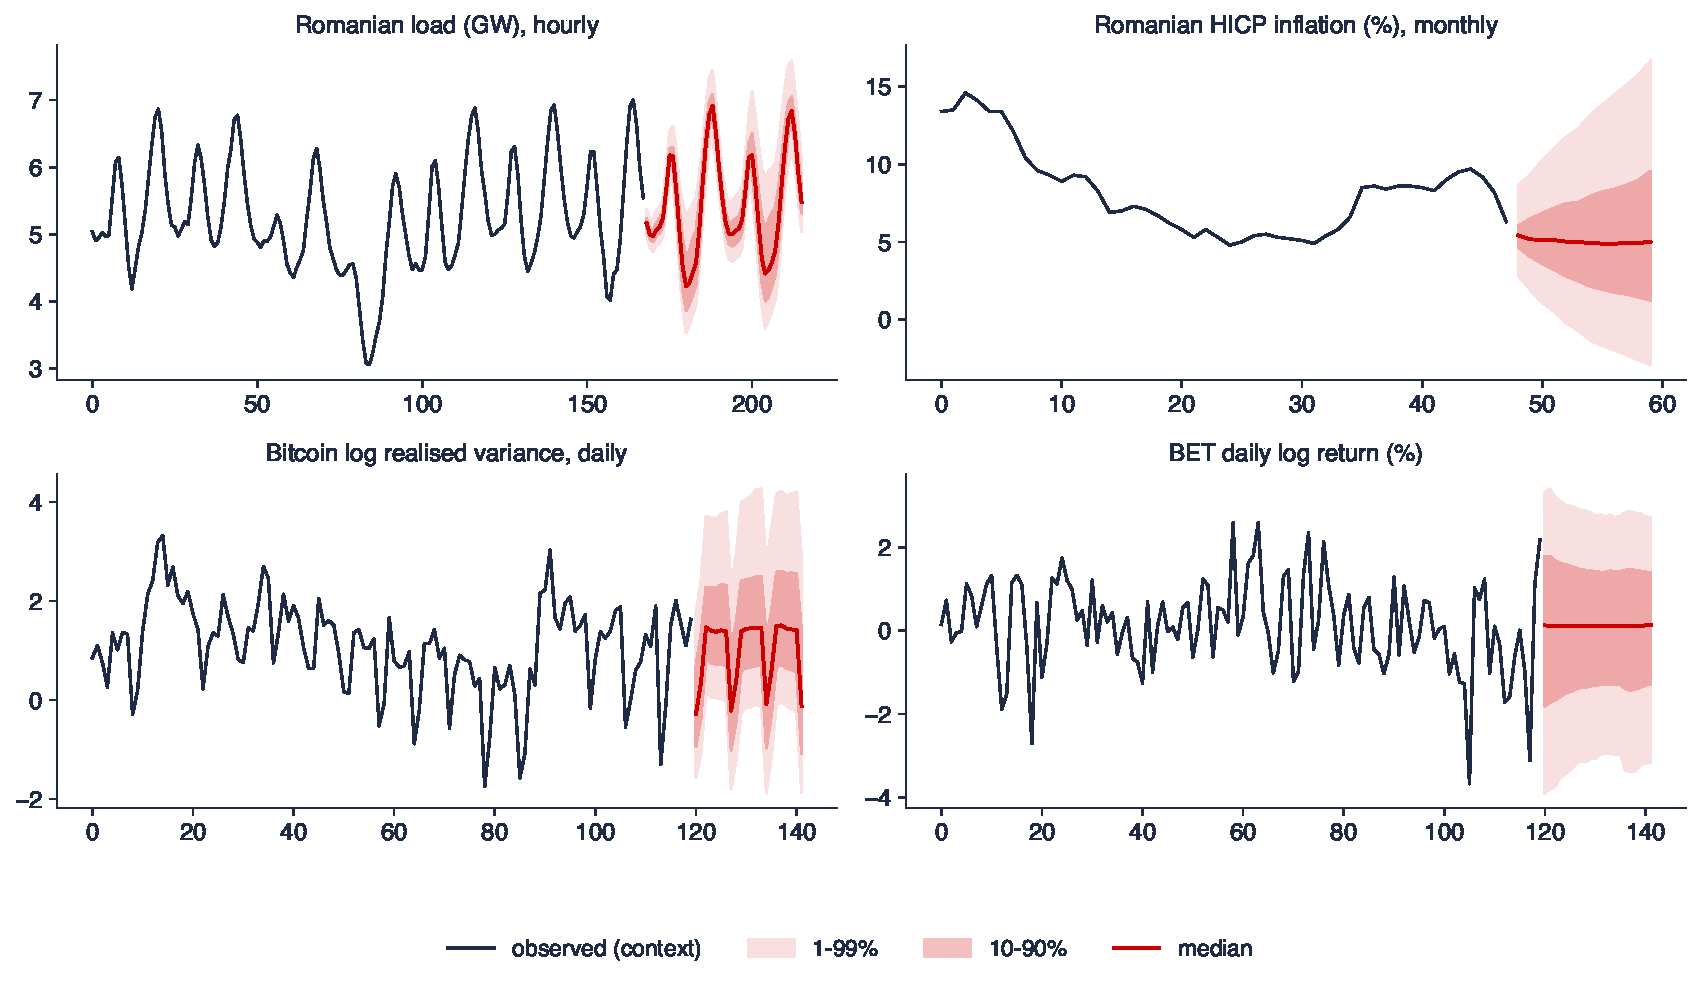
\includegraphics[width=0.97\textwidth,height=0.55\textheight,keepaspectratio]{ats_ch13_zeroshot.pdf}
\end{center}
\vspace{-0.25cm}
\begin{itemize}
    \item Chronos-2 from the last origin of each data set: Romanian load (48 hours), Romanian HICP inflation (12 months), Bitcoin log realised variance and BET daily returns (22 days); bands 10--90\% and 1--99\%
\end{itemize}
\quantlet{ATS\_ch13\_zero\_shot}{\qlurl{ATS_ch13_zero_shot}}
\end{frame}

\begin{frame}{Interpreting the four forecasts}
\itemsize{\small}
\begin{itemize}
    \item Load: the daily and weekly shapes are continued with narrow bands: shape transfer at its best
    \item Inflation: a smooth path towards the recent level with bands that widen with the horizon: close to what an AR model with persistence would give
    \item Log RV of Bitcoin: a weekly pattern (lower variance at weekends) around a level set by the context; returns: a flat median and a symmetric band, i.e.\ an unconditional distribution
    \item Return bands from the 1\% and 99\% quantiles: Chronos-2 VaR 1\% for the next day is 3.90 (\% of value); Section 8 checks whether such numbers are calibrated
\end{itemize}
\end{frame}

\begin{frame}{Recap: model families}
\itemsize{\small}
\begin{itemize}
    \item Families differ in input (tokens, patches, lags), architecture (encoder, decoder, recurrent) and output (categorical, quantiles, parametric)
    \item Quantile range is a design constraint: deciles only, except Chronos-2
    \item Zero-shot is the default; covariates in context and cross-learning are the new levers; closed APIs cannot be audited
\end{itemize}
\end{frame}


%=============================================================================
\section{Benchmarks, contamination and testing}
%=============================================================================

\begin{frame}{Benchmarks for pretrained models}
\itemsize{\small}
\begin{itemize}
    \item \textbf{GIFT-Eval} \refAks: 23 data sets, over 144\,000 series, 177 million points, seven domains, ten frequencies, short to long horizons; a non-leaking pretraining set
    \item \textbf{fev-bench} \refShc: 100 tasks in seven domains, 46 with covariates; win rates and skill scores with bootstrap confidence intervals
    \item \textbf{Live benchmarks}: forecasts registered before the outcomes exist, e.g.\ TS-Arena \refMey{} and Impermanent \refGarB: the only design immune to contamination by construction
    \item Classical references for what a fair comparison needs: M5 \refMak; pitfalls catalogued by \refHAB
\end{itemize}
\end{frame}

\begin{frame}{Aggregating scores across series}
\itemsize{\small}
\begin{itemize}
    \item Scale-free scores: MASE $= \frac{1}{H}\sum_h|y_{T+h} - \hat y_{T+h}| \big/ \frac{1}{T-m}\sum_t|y_t - y_{t-m}|$ \refHK; WQL $= 2\sum_{t,\tau}\rho_\tau(y_t - \hat q_{\tau,t})\big/\sum_t|y_t|$
    \begin{itemize}
        \item $\rho_\tau(u) = u(\tau - \mathbf 1\{u < 0\})$ (pinball); the average over $\tau$ approximates the CRPS (\atschlink{https://danpele.github.io/Advanced-Time-Series/EN/Courses/chapter1_forecast_evaluation.pdf}{Chapter 1})
    \end{itemize}
    \item Relative scores $r_s = L_s(\text{model})/L_s(\text{baseline})$ combined by the \textbf{geometric mean} \refFW: invariant to the choice of baseline in rankings, symmetric in gains and losses
    \begin{itemize}
        \item skill score $1 - \bar r_{\mathrm{geo}}$; win rate: share of series on which a model beats another
    \end{itemize}
    \item The arithmetic mean of ratios rewards the baseline's weak series; the mean of raw errors is dominated by the series with the largest scale
\end{itemize}
\end{frame}

\begin{frame}{Leakage and contamination}
\itemsize{\small}
\begin{itemize}
    \item \textbf{Series leakage}: an evaluation series (or a near copy) is in the pretraining corpus; Chronos separates in-domain (Benchmark I) from zero-shot (Benchmark II) results for this reason \refAns
    \item \textbf{Temporal contamination}: the test window precedes the training cutoff; the model may have seen the outcomes of other, correlated series in the same period
    \begin{itemize}
        \item LLMs recall exact economic values from before their cutoff \refLTZ; a two-data-set design against contamination for electricity prices \refPE
    \end{itemize}
    \item Designs that help
    \begin{itemize}
        \item evaluate only after the release (or the declared cutoff) of every model in the comparison; we use 1 November 2025, after the last of our models (Chronos-2, 30 October 2025)
        \item compare the relative skill before and after: a large drop after the release is a warning sign
        \item pre-register origins, horizons, metrics and baselines before looking at the results
    \end{itemize}
\end{itemize}
\end{frame}

\begin{frame}{Testing across many series}
\itemsize{\small}
\begin{itemize}
    \item One series: DM with HLN correction \refDM, \refHLN; conditional ability \refGW; many models: MCS \refHLNa{} (all in \atschlink{https://danpele.github.io/Advanced-Time-Series/EN/Courses/chapter1_forecast_evaluation.pdf}{Chapter 1})
    \item $S$ series tested separately: at 5\% each, about $0.05S$ false rejections are expected under the null
    \begin{itemize}
        \item \textbf{Holm} \refHol{} (FWER): order $p_{(1)} \le \dots \le p_{(S)}$, reject while $p_{(k)} \le \alpha/(S - k + 1)$
        \item \textbf{Benjamini--Hochberg} \refBH{} (FDR): reject the $k^*$ smallest, $k^* = \max\{k: p_{(k)} \le k\alpha/S\}$; valid under independence or positive dependence
    \end{itemize}
    \item Pooled tests: average the loss differential across series at each origin, then one DM test with HAC variance: the cross-sectional correlation is kept in the time dimension
    \item Ranks over many data sets: Friedman and Nemenyi tests \refDem; they ignore the size of differences and assume independent data sets
\end{itemize}
\end{frame}

\begin{frame}{Recap: benchmarks and testing}
\itemsize{\small}
\begin{itemize}
    \item Aggregate scale-free relative scores by geometric means and report uncertainty over series
    \item Contamination is a property of the pair (model, test window): evaluate after the release or live
    \item Many series mean many tests: correct with Holm or BH, or pool before testing
\end{itemize}
\end{frame}


%=============================================================================
\section{Evidence on our data}
%=============================================================================

\begin{frame}{The design of our comparisons}
\itemsize{\small}
\begin{itemize}
    \item \textbf{Romanian load}: day-ahead, 24 hours, every day from 1 January 2025 to 30 September 2026 (638 days); context 2048 hours for the foundation models
    \begin{itemize}
        \item baselines: weekly naive; the expert ARX of \refZW{} for each hour (\atschlink{https://danpele.github.io/Advanced-Time-Series/EN/Courses/chapter1_forecast_evaluation.pdf}{Chapter 1}); DLinear \refZen{} and N-BEATS \refOre{} trained globally (\atschlink{https://danpele.github.io/Advanced-Time-Series/EN/Courses/chapter12_machine_learning_deep_learning.pdf}{Chapter 12})
    \end{itemize}
    \item \textbf{EU inflation}: 27 countries, rolling monthly origins January 2012 -- August 2025, $h = 1, \dots, 12$; random walk, AR($p$) by AIC, damped ETS \refHKSG, DLinear and N-BEATS trained on the panel
    \item \textbf{Realised variance}: one day ahead, log RV; HAR \refCor{} on a rolling 1000-day window; QLIKE \refPat
    \item Foundation models: Chronos-Bolt small, Chronos-2, TimesFM 2.5, TiRex, zero-shot, on a CPU; Moirai and Lag-Llama were not run (their libraries need older software versions)
\end{itemize}
\end{frame}

\begin{frame}{Romanian load: day-ahead accuracy}
\itemsize{\footnotesize}
\begin{center}
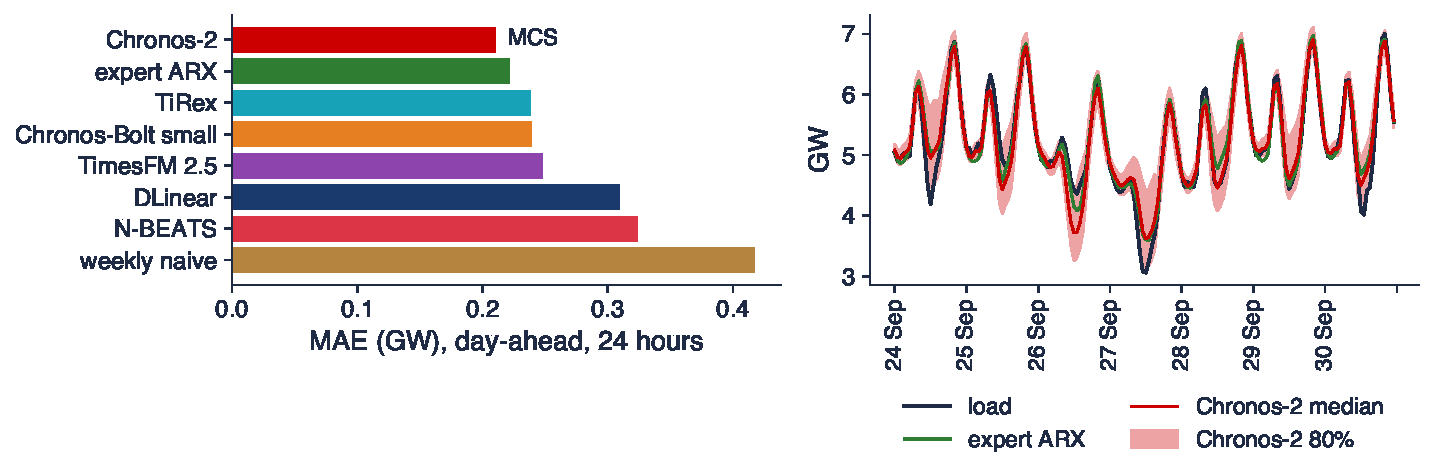
\includegraphics[width=0.97\textwidth,height=0.5\textheight,keepaspectratio]{ats_ch13_load.pdf}
\end{center}
\vspace{-0.25cm}
\begin{itemize}
    \item Left: MAE (GW) over 24 hours and 638 days, models in the 10\% MCS marked; right: the last week of the sample, expert ARX and Chronos-2 with its 80\% band
\end{itemize}
\quantlet{ATS\_ch13\_zero\_shot}{\qlurl{ATS_ch13_zero_shot}}
\end{frame}

\begin{frame}{Interpreting the load comparison}
\itemsize{\small}
\begin{itemize}
    \item MAE: Chronos-2 0.210, expert ARX 0.221, TiRex 0.238, Chronos-Bolt 0.239, TimesFM 0.248; DLinear 0.311, N-BEATS 0.325, weekly naive 0.417 GW
    \item DM against the expert ARX: Chronos-2 $t = \ensuremath{-}3.05$ ($p$ = 0.002); the other three foundation models are significantly worse; the 10\% MCS is \{Chronos-2\}
    \item 80\% interval coverage: Chronos-2 75.5\%, Chronos-Bolt 81.2\%, TimesFM 81.2\%, expert ARX 78.1\%: none is far off, none is exact
    \item A univariate zero-shot model matches an established domain model on a series with strong, regular shapes; the global deep models trained on three years lose to both
\end{itemize}
\end{frame}

\begin{frame}{In-context covariates: calendar and temperature}
\itemsize{\footnotesize}
\begin{center}
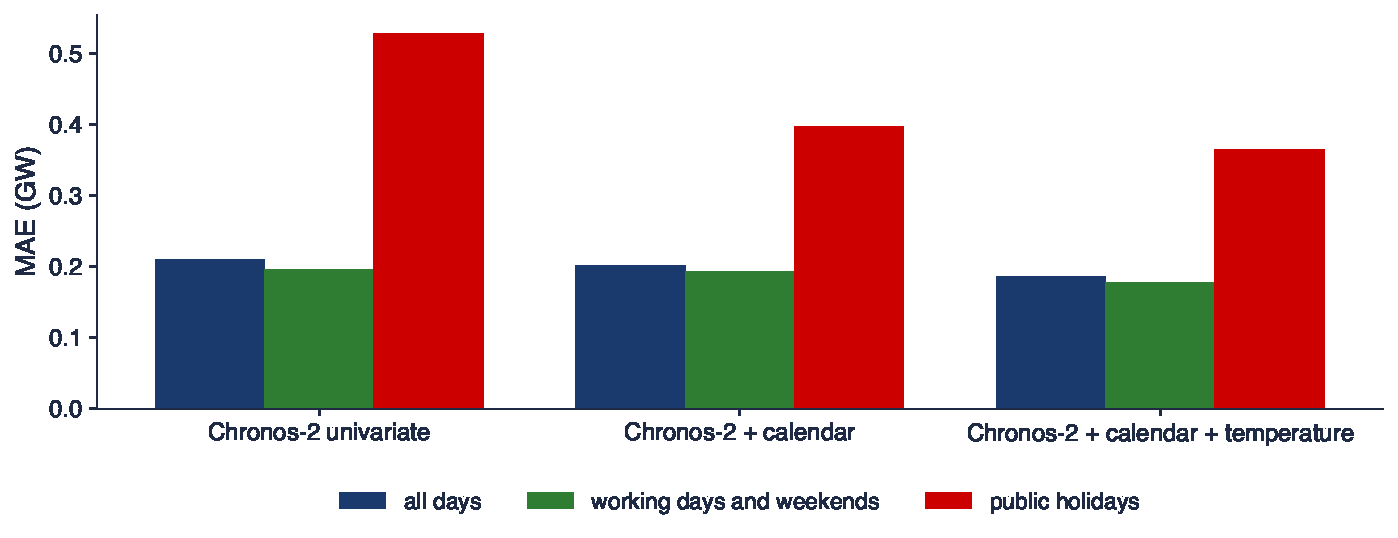
\includegraphics[width=0.97\textwidth,height=0.5\textheight,keepaspectratio]{ats_ch13_covariates.pdf}
\end{center}
\vspace{-0.25cm}
\begin{itemize}
    \item Chronos-2 MAE on all days, on ordinary days and on the 29 public holidays: univariate, with weekend and holiday flags, and with flags plus Bucharest hourly temperature (realised values for the forecast day: an upper bound)
\end{itemize}
\quantlet{ATS\_ch13\_zero\_shot}{\qlurl{ATS_ch13_zero_shot}}
\end{frame}

\begin{frame}{Interpreting the covariate experiment}
\itemsize{\small}
\begin{itemize}
    \item Holidays: MAE 0.527 univariate, 0.396 with the calendar, 0.365 with temperature; ordinary days: 0.195, 0.193, 0.178
    \item Calendar against univariate: DM $t = \ensuremath{-}2.79$ ($p$ = 0.005); temperature on top: $t = \ensuremath{-}7.02$ ($p$ $<$ 0.001)
    \item The holiday effect is learned in context from a few earlier holidays in the 2048-hour window; no parameter was estimated
    \item Realised temperature is not available at the origin: an operational test needs archived weather forecasts
\end{itemize}
\end{frame}

\begin{frame}{EU inflation: 27 countries, 12 horizons}
\itemsize{\footnotesize}
\begin{center}
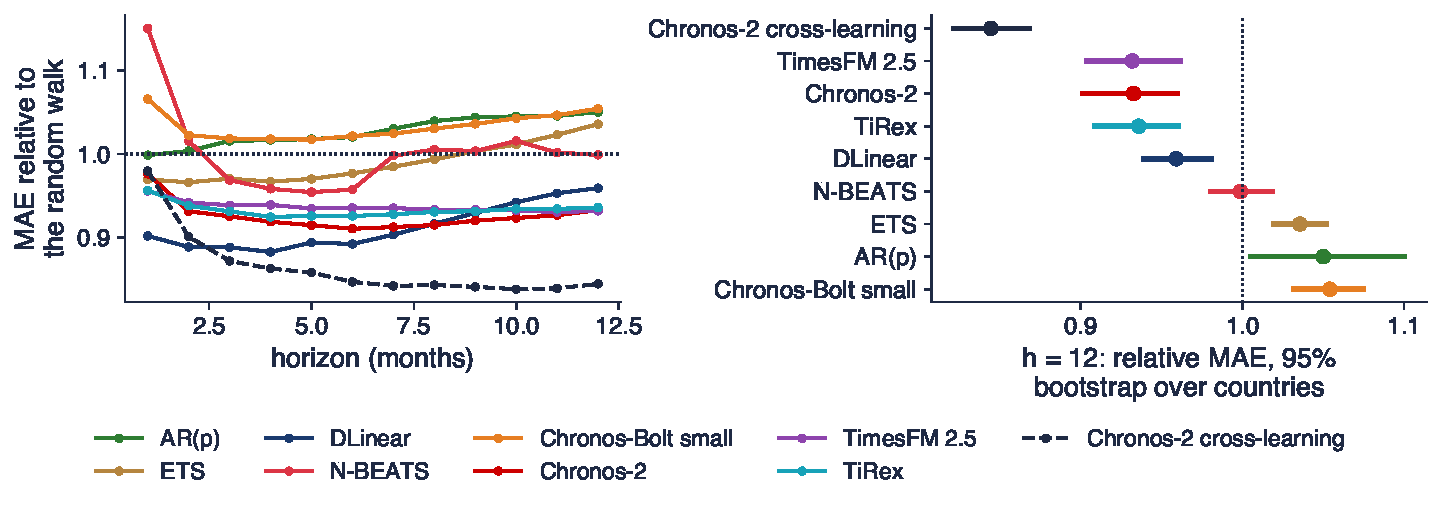
\includegraphics[width=0.97\textwidth,height=0.5\textheight,keepaspectratio]{ats_ch13_inflation.pdf}
\end{center}
\vspace{-0.25cm}
\begin{itemize}
    \item Left: MAE relative to the random walk by horizon, geometric mean over countries; right: $h = 12$ with 95\% bootstrap intervals over countries; origins January 2012 -- August 2025
\end{itemize}
\quantlet{ATS\_ch13\_benchmark}{\qlurl{ATS_ch13_benchmark}}
\end{frame}

\begin{frame}{Interpreting the inflation panel}
\itemsize{\small}
\begin{itemize}
    \item $h = 1$: AR 0.999, Chronos-2 0.976, TimesFM 0.956, TiRex 0.956; $h = 12$: AR 1.050, ETS 1.036, Chronos-2 0.933, TimesFM 0.932, TiRex 0.936, Bolt 1.054
    \item Global deep models at $h = 12$: DLinear 0.959, N-BEATS 0.999; Chronos-2 with cross-learning across the 27 countries: 0.845
    \item CRPS relative to AR (geometric mean over countries): Chronos-2 0.860, TimesFM 0.875, TiRex 0.865, ETS 0.972
    \item The 2021--2023 surge dominates every average: no univariate method foresaw it, so differences are about the speed of adaptation, not about foresight
\end{itemize}
\end{frame}

\begin{frame}{Romania: forecasts from three origins}
\itemsize{\footnotesize}
\begin{center}
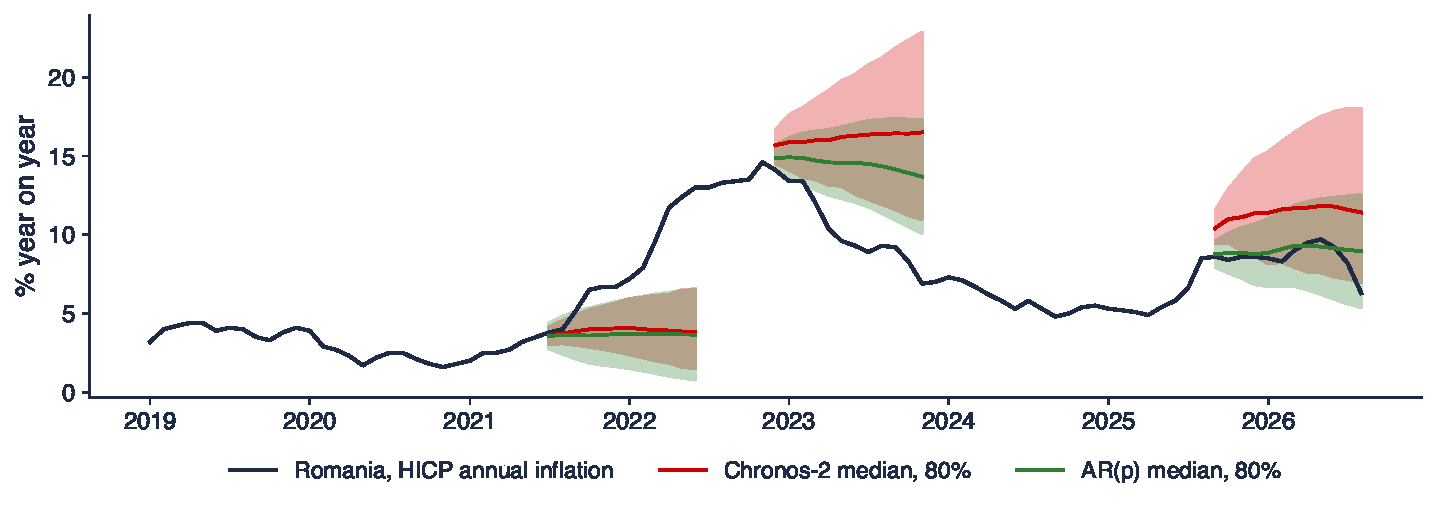
\includegraphics[width=0.97\textwidth,height=0.5\textheight,keepaspectratio]{ats_ch13_ro_inflation.pdf}
\end{center}
\vspace{-0.25cm}
\begin{itemize}
    \item Romanian HICP annual inflation and 12-month forecasts with 80\% bands from Chronos-2 and AR($p$), from June 2021, November 2022 and August 2025
\end{itemize}
\quantlet{ATS\_ch13\_benchmark}{\qlurl{ATS_ch13_benchmark}}
\end{frame}

\begin{frame}{Interpreting the Romanian paths}
\itemsize{\small}
\begin{itemize}
    \item From June 2021: 12 months later inflation was 13.0\%; Chronos-2 median 3.8\% (80\%: 1.5 -- 6.6), AR 3.7\%
    \item From November 2022, near the peak (14.6\% in November 2022): outcome 6.9\%; Chronos-2 16.5\%, AR 13.7\%
    \item From August 2025: outcome 6.3\%; Chronos-2 11.4\%, AR 9.0\%; the latest observation is 6.3\% (August 2026)
    \item Both methods extrapolate persistence; turning points come from information outside the series (energy prices, the end of the price caps, the VAT increase of August 2025, whose effect on annual inflation lasts exactly 12 months): known in advance, hence natural covariates
\end{itemize}
\end{frame}

\begin{frame}{Twenty-seven tests at once}
\itemsize{\footnotesize}
\begin{center}
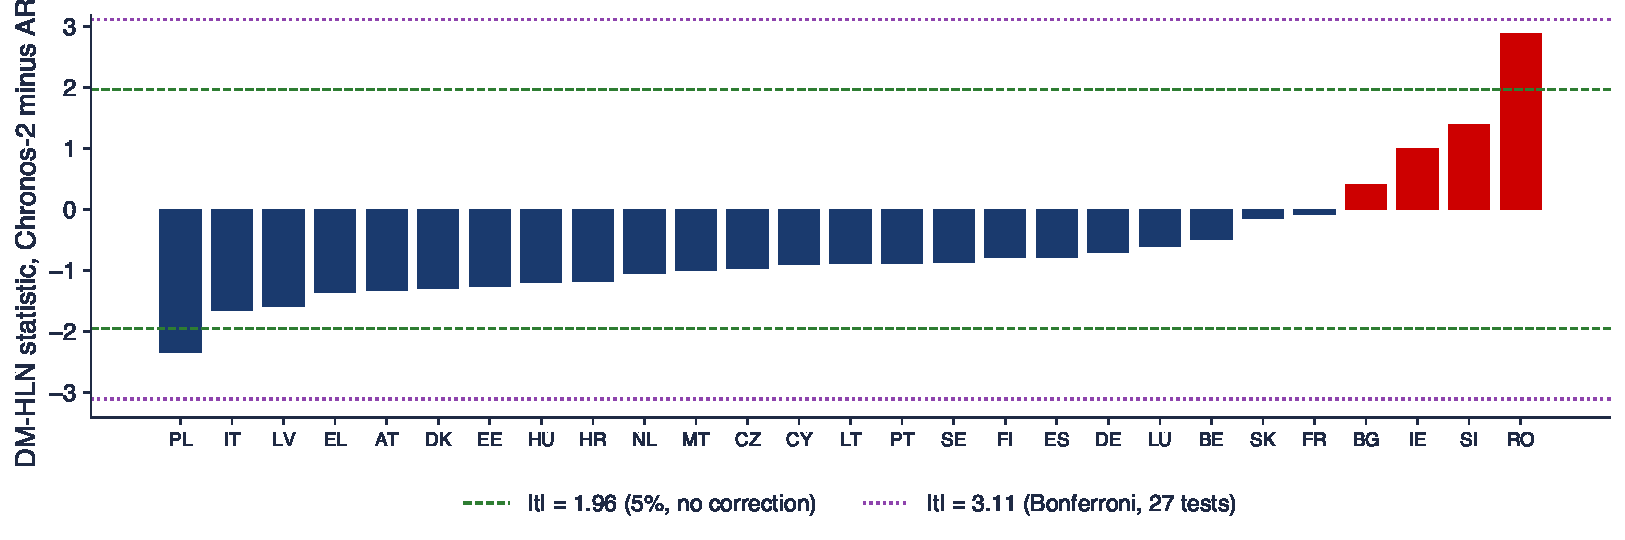
\includegraphics[width=0.97\textwidth,height=0.48\textheight,keepaspectratio]{ats_ch13_multiple.pdf}
\end{center}
\vspace{-0.25cm}
\begin{itemize}
    \item Country-level DM--HLN statistics (HAC with $h - 1$ lags) of the absolute errors of Chronos-2 minus AR($p$) at $h = 12$; negative: Chronos-2 better
\end{itemize}
\quantlet{ATS\_ch13\_benchmark}{\qlurl{ATS_ch13_benchmark}}
\end{frame}

\begin{frame}{Interpreting the multiple tests}
\itemsize{\small}
\begin{itemize}
    \item 23 of 27 statistics are negative; 2 are significant at 5\% without correction (1 in favour of Chronos-2, 1 in favour of AR)
    \item With Holm: 0 rejections; with Benjamini--Hochberg: 0; Romania: $t = 2.88$, $p$ = 0.005
    \item Pooled over the 27 countries (average loss differential at each origin, HAC variance): $t = \ensuremath{-}1.35$, $p$ = 0.180; the bootstrap intervals of the previous chart treat countries as independent and look sharper than they are
    \item A paper that reports the countries where its model wins at 5\% reports noise; the pooled test and the multiplicity-adjusted counts are the honest summary
\end{itemize}
\end{frame}

\begin{frame}{Realised variance: foundation models against HAR}
\itemsize{\footnotesize}
\begin{center}
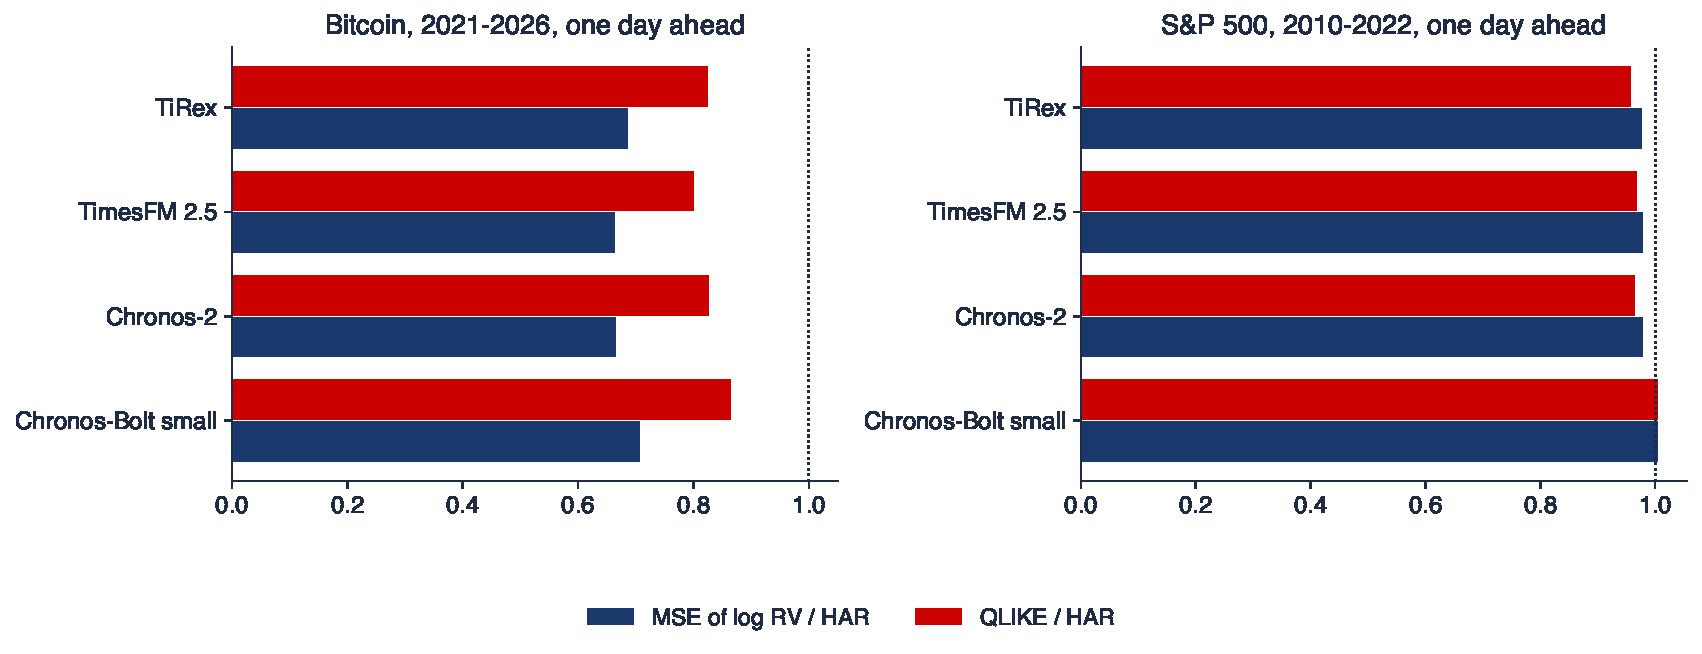
\includegraphics[width=0.97\textwidth,height=0.5\textheight,keepaspectratio]{ats_ch13_rv.pdf}
\end{center}
\vspace{-0.25cm}
\begin{itemize}
    \item One-day-ahead log RV: MSE and QLIKE relative to HAR; Bitcoin (Binance, 1 January 2021 -- 18 September 2026, $n = 2\,084$), S\&P 500 (Oxford-Man, 4 January 2010 -- 25 February 2022, $n = 3\,047$)
\end{itemize}
\quantlet{ATS\_ch13\_benchmark}{\qlurl{ATS_ch13_benchmark}}
\end{frame}

\begin{frame}{Interpreting the volatility comparison}
\itemsize{\small}
\begin{itemize}
    \item Bitcoin, QLIKE relative to HAR: Chronos-2 0.825, TimesFM 0.800, TiRex 0.824, Bolt 0.864; MCS (10\%): \{Chronos-2, TimesFM 2.5, TiRex\}
    \item S\&P 500: Chronos-2 0.963, TimesFM 0.968, TiRex 0.956, Bolt 1.004; MCS (10\%): \{Chronos-2, TimesFM 2.5, TiRex\}
    \item Three of the four zero-shot models beat HAR on both assets and HAR is outside both MCS: the slowly decaying memory of log RV (\atschlink{https://danpele.github.io/Advanced-Time-Series/EN/Courses/chapter10_long_memory_rough_volatility.pdf}{Chapter 10}) is a shape a corpus can teach; the gain is large for Bitcoin, small for the S\&P 500
    \item Recent studies reach mixed verdicts \refGoe, \refBri, \refRNW: gains depend on the asset, the horizon and the loss, and fine-tuning or pretraining on financial data often matters
\end{itemize}
\end{frame}

\begin{frame}{Before and after the releases}
\itemsize{\footnotesize}
\begin{center}
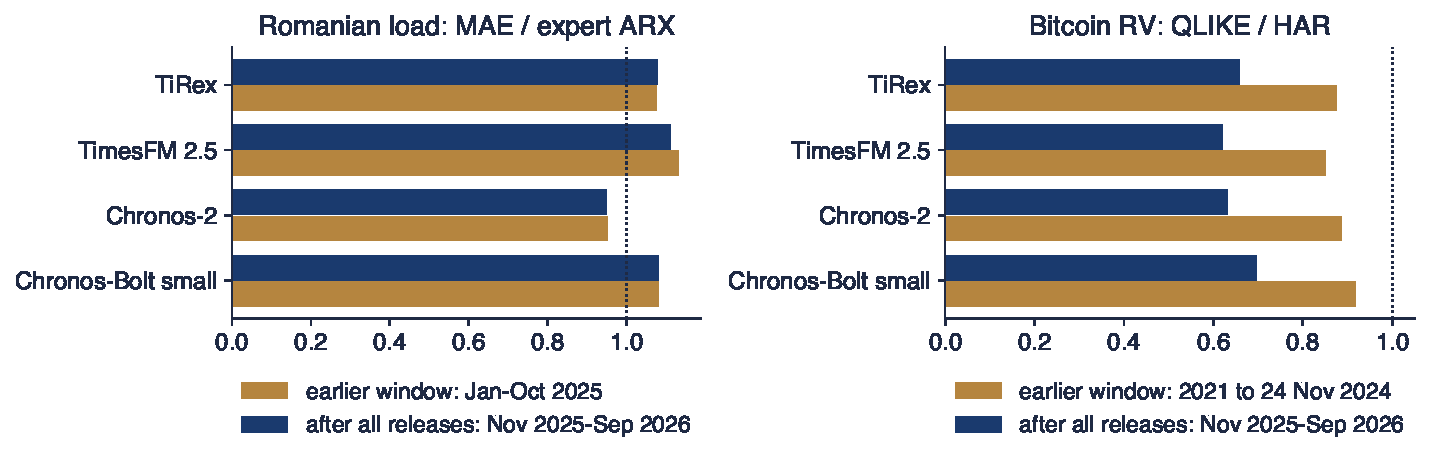
\includegraphics[width=0.97\textwidth,height=0.5\textheight,keepaspectratio]{ats_ch13_contamination.pdf}
\end{center}
\vspace{-0.25cm}
\begin{itemize}
    \item Relative loss of each model in an earlier window and in the window after every release (from 1 November 2025): load (MAE / expert ARX) and Bitcoin (QLIKE / HAR)
\end{itemize}
\quantlet{ATS\_ch13\_benchmark}{\qlurl{ATS_ch13_benchmark}}
\end{frame}

\begin{frame}{Interpreting the contamination check}
\itemsize{\small}
\begin{itemize}
    \item Load, Chronos-2: 0.952 before, 0.950 after; TimesFM: 1.133, 1.112; the earlier window (January--October 2025) precedes both releases
    \item Bitcoin, Chronos-2: 0.886 (2021 -- 24 November 2024) and 0.631 (after); TiRex: 0.874, 0.658; post-release windows have 334 and 322 days
    \item No deterioration after the releases (for Bitcoin the ratios are even lower): no evidence of contamination here; but the absence of a drop does not prove absence of leakage, and markets change between windows
\end{itemize}
\end{frame}

\begin{frame}{Recap: the evidence}
\itemsize{\small}
\begin{itemize}
    \item Strong shapes (load): the best foundation model matches or beats the domain model; weak shapes (returns): little to transfer
    \item Inflation: ahead of AR and ETS in the panel average (most with cross-learning), but no country difference survives Holm or BH and the pooled test is not significant
    \item Realised variance: zero-shot models beat HAR, clearly for Bitcoin, narrowly for the S\&P 500
    \item Covariates in context help where the calendar matters; post-release windows show no sign of contamination
\end{itemize}
\end{frame}


%=============================================================================
\section{Language models for time series}
%=============================================================================

\begin{frame}{LLMTime: numbers as text}
\itemsize{\small}
\begin{itemize}
    \item \refGru: rescale, round to a fixed number of digits, write values as digits separated by spaces and commas; an off-the-shelf LLM continues the string
    \begin{itemize}
        \item digit-by-digit probabilities define a hierarchical (multi-bin) density over continuous values; repeated sampling gives quantiles
    \end{itemize}
    \item Findings of the paper: competitive zero-shot on some benchmarks; tokenisation of numbers matters (a newer model could do worse because of how it splits digits); alignment (RLHF) hurts calibration
    \item Costs: thousands of tokens per series and many samples per forecast; the context window limits the history; the LLM may have memorised the data
\end{itemize}
\end{frame}

\begin{frame}{Reprogramming a frozen LLM}
\itemsize{\small}
\begin{itemize}
    \item \textbf{Time-LLM} \refJin: patches of the series are mapped onto text prototypes (word embeddings), a prompt prefix describes the task and statistics; the LLM stays frozen, a projection reads the forecast
    \item \textbf{One Fits All} (GPT4TS) \refZho: a frozen GPT-2 with trained input embedding, layer norms and output layer, for forecasting, classification and anomaly detection
    \item The claim: knowledge from language transfers to series; the test of the claim is an ablation that removes the language model
\end{itemize}
\end{frame}

\begin{frame}{Case study: are language models actually useful?}
\itemsize{\small}
\begin{columns}[T]
\begin{column}{0.56\textwidth}
\begin{itemize}
    \item \refTan: three LLM-based forecasters (including Time-LLM and GPT4TS), the same benchmarks, three ablations
    \item Ablations
    \begin{itemize}
        \item remove the LLM; replace it by one attention layer; replace it by a basic Transformer block
    \end{itemize}
    \item Result: no degradation, often an improvement; pretrained LLMs do no better than the same model trained from scratch, do not model sequential dependence, do not help in few-shot settings
    \item Training and inference cost orders of magnitude more
\end{itemize}
\end{column}
\begin{column}{0.42\textwidth}
\begin{itemize}
    \item The method matters more than the result
    \item an architecture claim needs an ablation with matched compute and tuning
    \item time-series foundation models trained on series (Chronos, TimesFM, TiRex) are not affected by this critique; LLMs used as forecasters are
    \item LLMs remain useful around forecasting: code, literature, critique (Section 9)
\end{itemize}
\end{column}
\end{columns}
\end{frame}

\begin{frame}{Memorisation and look-ahead}
\itemsize{\small}
\begin{itemize}
    \item \refLTZ: LLMs reproduce macroeconomic and market values from their training period with high precision, even when asked not to use future information
    \begin{itemize}
        \item a backtest before the training cutoff measures recall, not forecasting
    \end{itemize}
    \item For time-series foundation models the same logic applies to public series in the corpus (electricity, traffic, M4)
    \begin{itemize}
        \item our evidence: windows after every release (Section 4); the strongest evidence: live, pre-registered forecasts
    \end{itemize}
    \item A practical rule: state the training cutoff of every model and the start of the evaluation window in the same table
\end{itemize}
\end{frame}

\begin{frame}{Recap: LLMs}
\itemsize{\small}
\begin{itemize}
    \item LLMTime and reprogramming show that text models can be bent to series; ablations show the language part is rarely what helps
    \item Memorisation makes pre-cutoff evaluation of LLM forecasts invalid
\end{itemize}
\end{frame}


%=============================================================================
\section{Conformal prediction}
%=============================================================================

\begin{frame}{Where conformal prediction comes from}
\itemsize{\small}
\begin{columns}[T]
\begin{column}{0.42\textwidth}
\centering
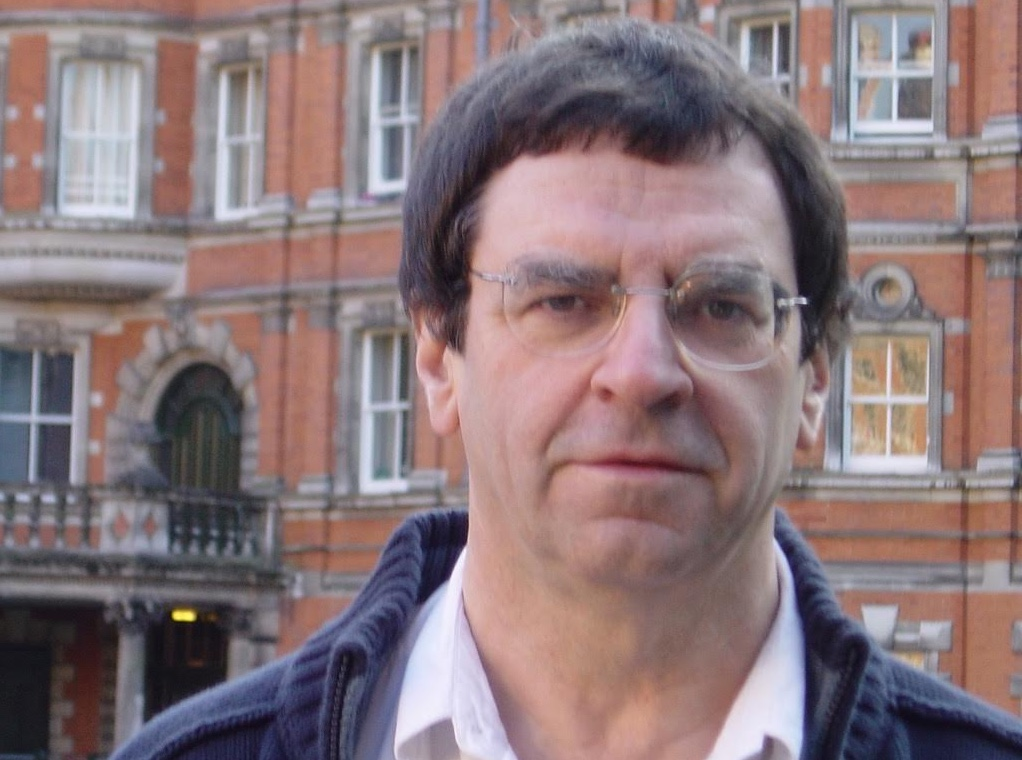
\includegraphics[height=0.36\textheight]{ch13_gammerman_2018.jpg}\\[1mm]
\imgcap{Alexander Gammerman, Royal Holloway, 2018}
\imgcredit{https://commons.wikimedia.org/wiki/File:Alexander-Gammerman-professor-at-RHUL.jpg}{Photo: Jaguar224 (2018); CC BY-SA 4.0; Wikimedia Commons}
\end{column}
\begin{column}{0.56\textwidth}
\begin{itemize}
    \item Vovk, Gammerman and Shafer \refVGS, \refVGSb: prediction sets valid in finite samples under exchangeability only, for any predictive model
    \item The idea: how "conforming" a candidate value is to the data seen, measured by a rank
    \item Modern statistics adopted it as a wrapper around machine learning \refLei, \refAB
\end{itemize}
\end{column}
\end{columns}
\end{frame}

\begin{frame}{Exchangeability and the target guarantee}
\itemsize{\small}
\begin{itemize}
    \item $Z_1, \dots, Z_{n+1}$, $Z_i = (X_i, Y_i)$, are \textbf{exchangeable} if $(Z_{\pi(1)}, \dots, Z_{\pi(n+1)}) \overset{d}{=} (Z_1, \dots, Z_{n+1})$ for every permutation $\pi$
    \begin{itemize}
        \item i.i.d.\ implies exchangeable; draws without replacement are exchangeable but dependent; a stationary AR(1) is not exchangeable
    \end{itemize}
    \item \textbf{Marginal coverage}: $\Pr\{Y_{n+1} \in \hat C(X_{n+1})\} \ge 1 - \alpha$, the probability taken over the calibration data and the test point together
    \begin{itemize}
        \item not \textbf{conditional} coverage $\Pr\{Y \in \hat C(x) \mid X = x\} \ge 1 - \alpha$ for every $x$, and not coverage given the calibration sample
    \end{itemize}
    \item A \textbf{nonconformity score} $s(x, y)$: large when $y$ is unusual given $x$, e.g.\ $|y - \hat\mu(x)|$, $|y - \hat\mu(x)|/\hat\sigma(x)$, or the CQR score below
\end{itemize}
\end{frame}

\begin{frame}{Split conformal prediction}
\itemsize{\small}
\begin{itemize}
    \item Fit $\hat\mu$ on a training set; compute $S_i = s(X_i, Y_i)$ on $n$ calibration points \refPap, \refLei
    \begin{itemize}
        \item $\hat q = S_{(k)}$, $k = \lceil (n + 1)(1 - \alpha) \rceil$ (the $k$-th smallest; $+\infty$ if $k > n$); $\hat C(x) = \{y: s(x, y) \le \hat q\}$
    \end{itemize}
    \item \textbf{Theorem}: if $(X_i, Y_i)_{i \le n+1}$ are exchangeable, $\Pr\{Y_{n+1} \in \hat C(X_{n+1})\} \ge 1 - \alpha$; with no ties, also $\le 1 - \alpha + 1/(n + 1)$
    \begin{itemize}
        \item proof: given $\hat\mu$, the scores $S_1, \dots, S_{n+1}$ are exchangeable, so the rank of $S_{n+1}$ is uniform on $\{1, \dots, n + 1\}$; $Y_{n+1} \in \hat C \iff$ rank $\le k$, probability $k/(n + 1) \ge 1 - \alpha$ (\atsapplink{atsapp1}{atssrc1}{Appendix})
    \end{itemize}
    \item No assumption on the model or on the distribution: a bad model gives wide, not invalid, intervals
\end{itemize}
\end{frame}

\begin{frame}{Coverage given the calibration set}
\itemsize{\footnotesize}
\begin{center}
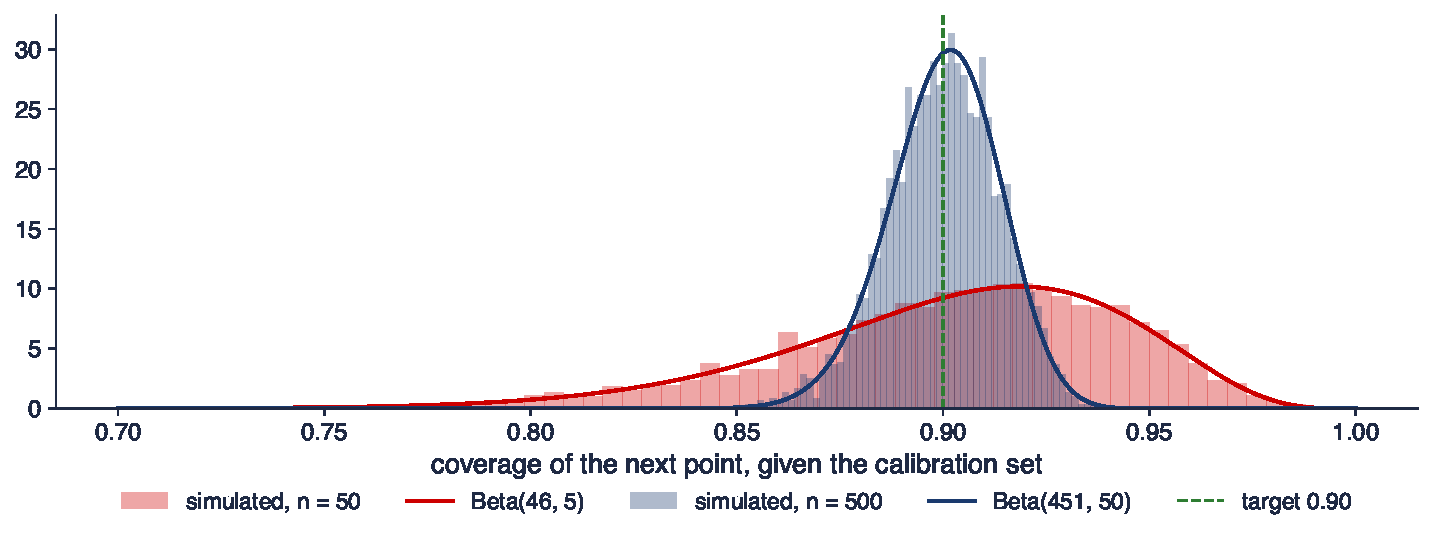
\includegraphics[width=0.97\textwidth,height=0.48\textheight,keepaspectratio]{ats_ch13_split_coverage.pdf}
\end{center}
\vspace{-0.25cm}
\begin{itemize}
    \item Coverage $F(\hat q)$ of the next point for 4000 calibration sets of $n = 50$ and $n = 500$ scores, $\alpha = 0.1$, and the exact law Beta($k$, $n + 1 - k$)
\end{itemize}
\quantlet{ATS\_ch13\_conformal\_basics}{\qlurl{ATS_ch13_conformal_basics}}
\end{frame}

\begin{frame}{Interpreting the coverage distribution}
\itemsize{\small}
\begin{itemize}
    \item Mean coverage 0.902 ($n = 50$) and 0.900 ($n = 500$), as the theory gives (0.902, 0.900): the marginal guarantee holds on average over calibration sets
    \item One calibration set is one draw: s.d.\ 0.041 and 0.014; with $n = 50$, 26\% of the sets give coverage below 0.88, with $n = 500$ only 7\%
    \item Since $F(\hat q) \sim$ Beta($k$, $n + 1 - k$), choosing $n$ is a sample-size calculation: the s.d.\ is about $\sqrt{\alpha(1 - \alpha)/n}$
\end{itemize}
\end{frame}

\begin{frame}{Conformalized quantile regression}
\itemsize{\small}
\begin{columns}[T]
\begin{column}{0.32\textwidth}
\centering

\includegraphics[height=0.34\textheight]{ch13_candes_2012.jpg}\\[1mm]
\imgcap{Emmanuel Candès, 2012}
\imgcredit{https://commons.wikimedia.org/wiki/File:Emmanuel_Cand\%C3\%A8s.jpg}{Photo: Renate Schmid, MFO (2012); CC BY-SA 2.0 de; Wikimedia Commons}
\end{column}
\begin{column}{0.66\textwidth}
\begin{itemize}
    \item \refRPC: fit quantile regressions \refKB{} $\hat q_{\alpha/2}(x)$, $\hat q_{1-\alpha/2}(x)$ on the training set
    \item Score $s(x, y) = \max\{\hat q_{\alpha/2}(x) - y,\; y - \hat q_{1-\alpha/2}(x)\}$: negative inside the band
    \item $\hat C(x) = [\hat q_{\alpha/2}(x) - \hat q,\; \hat q_{1-\alpha/2}(x) + \hat q]$: the band is shifted outwards (or inwards if $\hat q < 0$)
    \item Marginal coverage by the split theorem; the width adapts to heteroskedasticity through the quantile models
    \item The same score calibrates the quantiles of any foundation model (Section 8)
\end{itemize}
\end{column}
\end{columns}
\end{frame}

\begin{frame}{CQR on the design of Romano, Patterson and Candès}
\itemsize{\footnotesize}
\begin{center}
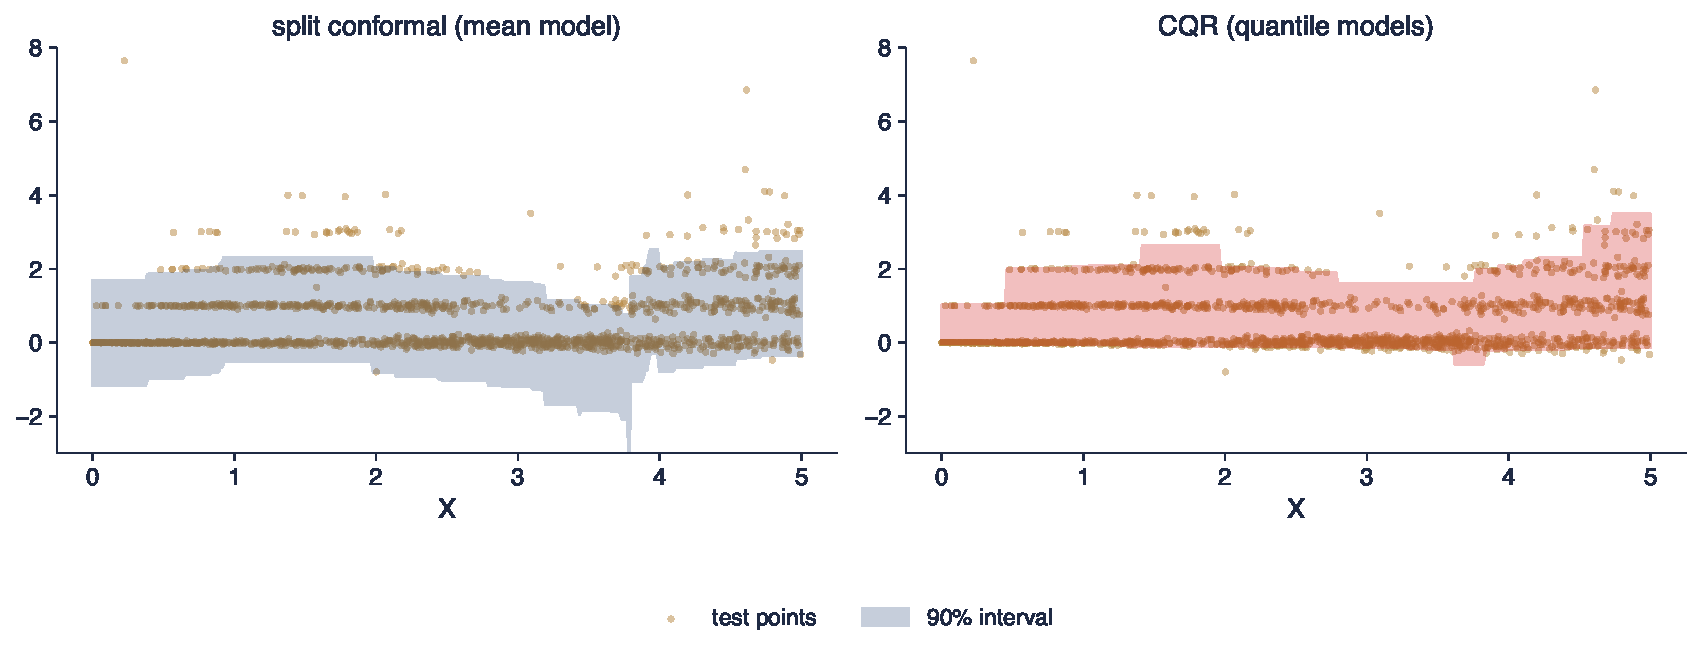
\includegraphics[width=0.97\textwidth,height=0.48\textheight,keepaspectratio]{ats_ch13_cqr.pdf}
\end{center}
\vspace{-0.25cm}
\begin{itemize}
    \item $Y = \mathrm{Pois}(\sin^2 X + 0.1) + 0.03X\varepsilon_1 + 25\cdot\mathbf 1\{U < 0.01\}\varepsilon_2$, $X \sim U[0, 5]$ (their Figure 1); 1000 training and 1000 calibration points; gradient boosting for the mean and for the 5\% and 95\% quantiles
\end{itemize}
\quantlet{ATS\_ch13\_conformal\_basics}{\qlurl{ATS_ch13_conformal_basics}}
\end{frame}

\begin{frame}{Interpreting CQR}
\itemsize{\small}
\begin{itemize}
    \item Test coverage: split conformal 0.918, CQR 0.915, the raw quantile models 0.883; mean width 2.84, 2.20 and 2.17
    \item The raw quantile regressions undercover; CQR repairs them at almost no extra width, while the constant-width split band is 29\% wider
    \item By $X$ bins both stay within a few points of 90\% (worst bins: CQR 0.892, split 0.896); the gain of CQR is in width: narrow where $Y$ is concentrated, wide where the Poisson noise is large
\end{itemize}
\end{frame}

\begin{frame}{The limits of conditional coverage}
\itemsize{\small}
\begin{itemize}
    \item \textbf{Impossibility} \refVov, \refLW, \refBarB: if $\hat C$ has conditional coverage $\ge 1 - \alpha$ at almost every $x$ for every distribution with a continuous $X$, then its expected length is infinite
    \begin{itemize}
        \item no finite-sample method can certify coverage at each point of a continuous covariate without assumptions
    \end{itemize}
    \item What is achievable: coverage within a finite set of groups (Mondrian conformal: calibrate separately by group); approximate conditional coverage under smoothness; coverage conditional on the calibration set with high probability (Beta law)
    \item For time series the relevant condition is the past: $\Pr\{Y_t \in \hat C_t \mid \mathcal F_{t-1}\}$; a VaR backtest (\atschlink{https://danpele.github.io/Advanced-Time-Series/EN/Courses/chapter9_var_es_backtesting.pdf}{Chapter 9}) tests exactly this property for one-sided sets
\end{itemize}
\end{frame}

\begin{frame}{Recap: conformal prediction}
\itemsize{\small}
\begin{itemize}
    \item Split conformal: a rank argument gives finite-sample marginal coverage under exchangeability, for any model
    \item CQR adds adaptivity; the calibration sample size controls the variability of realised coverage
    \item Conditional coverage is impossible in general: test it, do not claim it
\end{itemize}
\end{frame}


%=============================================================================
\section{Conformal prediction for dependent data}
%=============================================================================

\begin{frame}{Exchangeability violated: what survives}
\itemsize{\small}
\begin{itemize}
    \item Time series violate exchangeability three ways: serial dependence, changing volatility, structural change; the last two break coverage most
    \item \textbf{Stationary and mixing}: split conformal remains approximately valid, with a coverage gap controlled by $\beta$-mixing coefficients and the calibration size \refOli
    \begin{itemize}
        \item block permutations restore exactness under weaker conditions \refCWZ
    \end{itemize}
    \item \textbf{Non-stationary}: no static method can work; the threshold must move with the data: weights (Barber et al.), refitting (EnbPI), feedback on errors (ACI, PID)
    \item A common online frame: scores $S_t = s(X_t, Y_t)$ computed from out-of-sample forecasts; at $t$ choose a threshold $q_t$ from $S_1, \dots, S_{t-1}$; miss $\mathrm{err}_t = \mathbf 1\{S_t > q_t\}$
\end{itemize}
\end{frame}

\begin{frame}{Conformal prediction beyond exchangeability}
\itemsize{\small}
\begin{itemize}
    \item \refBar: fixed weights $w_i \in [0, 1]$, chosen before seeing the data; $\hat q$ = the $(1 - \alpha)$ quantile of $\sum_i \tilde w_i\delta_{S_i} + \tilde w_{n+1}\delta_{+\infty}$, $\tilde w_i = w_i/(1 + \sum_j w_j)$, $w_{n+1} = 1$
    \begin{itemize}
        \item \textbf{Theorem}: coverage $\ge 1 - \alpha - \sum_i \tilde w_i\, d_{\mathrm{TV}}(Z, Z^i)$, where $Z^i$ swaps the test point with point $i$
    \end{itemize}
    \item Under exchangeability the gap is zero; under drift, $d_{\mathrm{TV}}$ is small for recent points, so geometric weights $w_i = \rho^{n+1-i}$ keep it small
    \begin{itemize}
        \item effective sample size $\approx 1/(1 - \rho)$: $\rho = 0.99$ uses about 100 recent scores; robustness against variance of the threshold
    \end{itemize}
    \item Covariate shift with known likelihood ratio: weights $w(x) = dP_{\mathrm{test}}/dP_{\mathrm{train}}$ give exact coverage \refTBCR
\end{itemize}
\end{frame}

\begin{frame}{Weighted conformal under changepoints}
\itemsize{\footnotesize}
\begin{center}
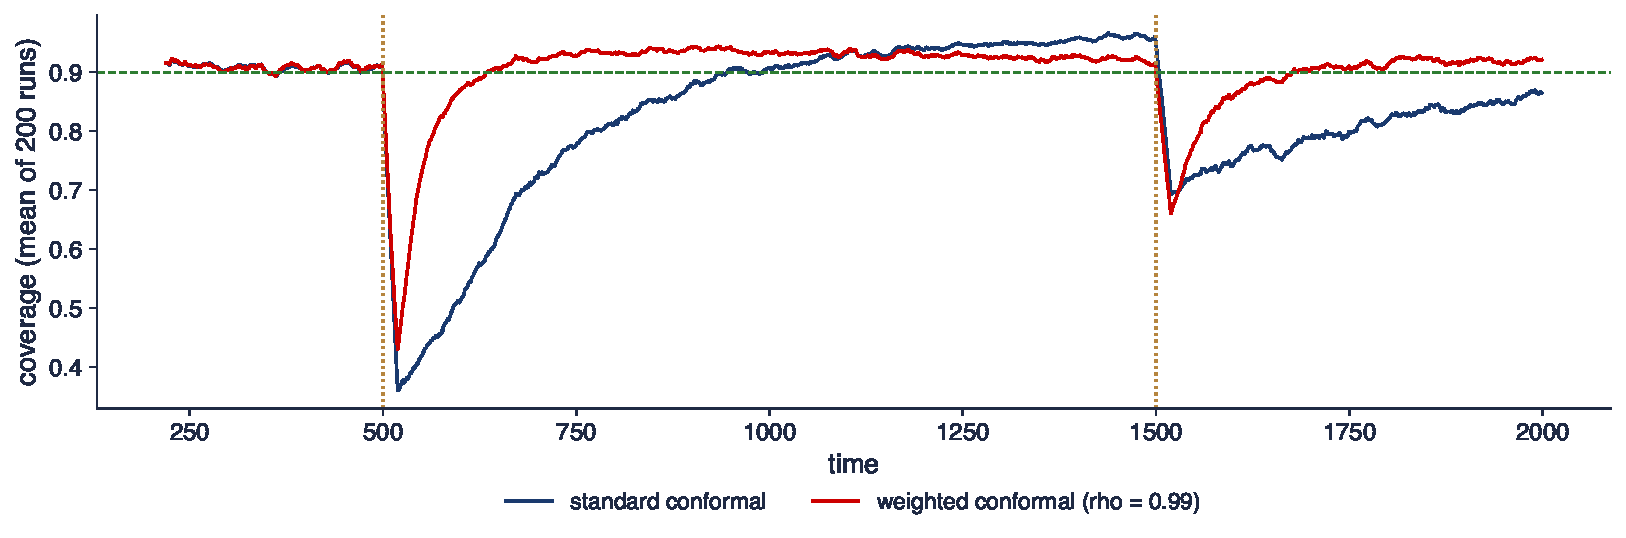
\includegraphics[width=0.97\textwidth,height=0.48\textheight,keepaspectratio]{ats_ch13_weighted.pdf}
\end{center}
\vspace{-0.25cm}
\begin{itemize}
    \item $Y_t = X_t'\beta_t + \varepsilon_t$, $X_t \sim N(0, I_4)$, $\beta$ changes at $t = 500$ and $t = 1500$; least squares on all past data; prequential absolute residuals as scores; coverage averaged over 200 runs (20-step moving average)
\end{itemize}
\quantlet{ATS\_ch13\_conformal\_time}{\qlurl{ATS_ch13_conformal_time}}
\end{frame}

\begin{frame}{Interpreting the weighted method}
\itemsize{\small}
\begin{itemize}
    \item Average coverage after the burn-in: standard 0.836, weighted ($\rho = 0.99$) 0.900; worst 20-step average 0.36 against 0.43
    \item Both collapse at a break, because the least-squares fit is wrong for a while; the weighted threshold forgets the old scores and recovers within about 100 steps
    \item Price: mean width 7.47 against 6.22; the guarantee is a bound in terms of $d_{\mathrm{TV}}$, not exact coverage
\end{itemize}
\end{frame}

\begin{frame}{EnbPI: ensembles without data splitting}
\itemsize{\small}
\begin{itemize}
    \item \refXX, \refXXb: fit $B$ models on bootstrap samples (blocks, to respect dependence) of the training period
    \begin{itemize}
        \item leave-one-out residuals: for point $i$, aggregate only the models whose bootstrap sample excluded $i$
        \item interval at $t$: $\hat f(x_t) \pm$ the $(1 - \alpha)$ quantile of the last $T$ absolute residuals; after $y_t$ is observed, its residual enters the window and the oldest leaves
    \end{itemize}
    \item No refitting at each step, no calibration split: efficient for long streams
    \item Guarantee: asymptotic, conditional coverage if the errors are stationary and strongly mixing and the ensemble is consistent; designed for energy series (solar and wind)
\end{itemize}
\end{frame}

\begin{frame}{Adaptive conformal inference}
\itemsize{\small}
\begin{itemize}
    \item \refGC: use level $\alpha_t$ at time $t$, $q_t$ = the conformal $(1 - \alpha_t)$ quantile of recent scores, then $\alpha_{t+1} = \alpha_t + \gamma(\alpha - \mathrm{err}_t)$
    \begin{itemize}
        \item a miss lowers $\alpha_t$ (wider sets); a hit raises it; $\alpha_t \le 0$ gives $q_t = +\infty$ (the whole line), $\alpha_t \ge 1$ the empty set
    \end{itemize}
    \item \textbf{Theorem}: for any sequence of data, $\Big|\frac1T\sum_{t=1}^T\mathrm{err}_t - \alpha\Big| \le \frac{\max\{\alpha_1, 1 - \alpha_1\} + \gamma}{\gamma T}$
    \begin{itemize}
        \item proof: $\alpha_t$ stays in $[-\gamma, 1 + \gamma]$ and $\alpha_{T+1} - \alpha_1 = \gamma\sum_t(\alpha - \mathrm{err}_t)$; divide by $\gamma T$
    \end{itemize}
    \item Long-run frequency, not conditional coverage: an adversary-proof average. Choosing $\gamma$ adaptively: AgACI \refZaf, DtACI \refGCb; ACI for VaR: \atschlink{https://danpele.github.io/Advanced-Time-Series/EN/Courses/chapter9_var_es_backtesting.pdf}{Chapter 9}
\end{itemize}
\end{frame}

\begin{frame}{ACI on stock-market volatility}
\itemsize{\footnotesize}
\begin{center}
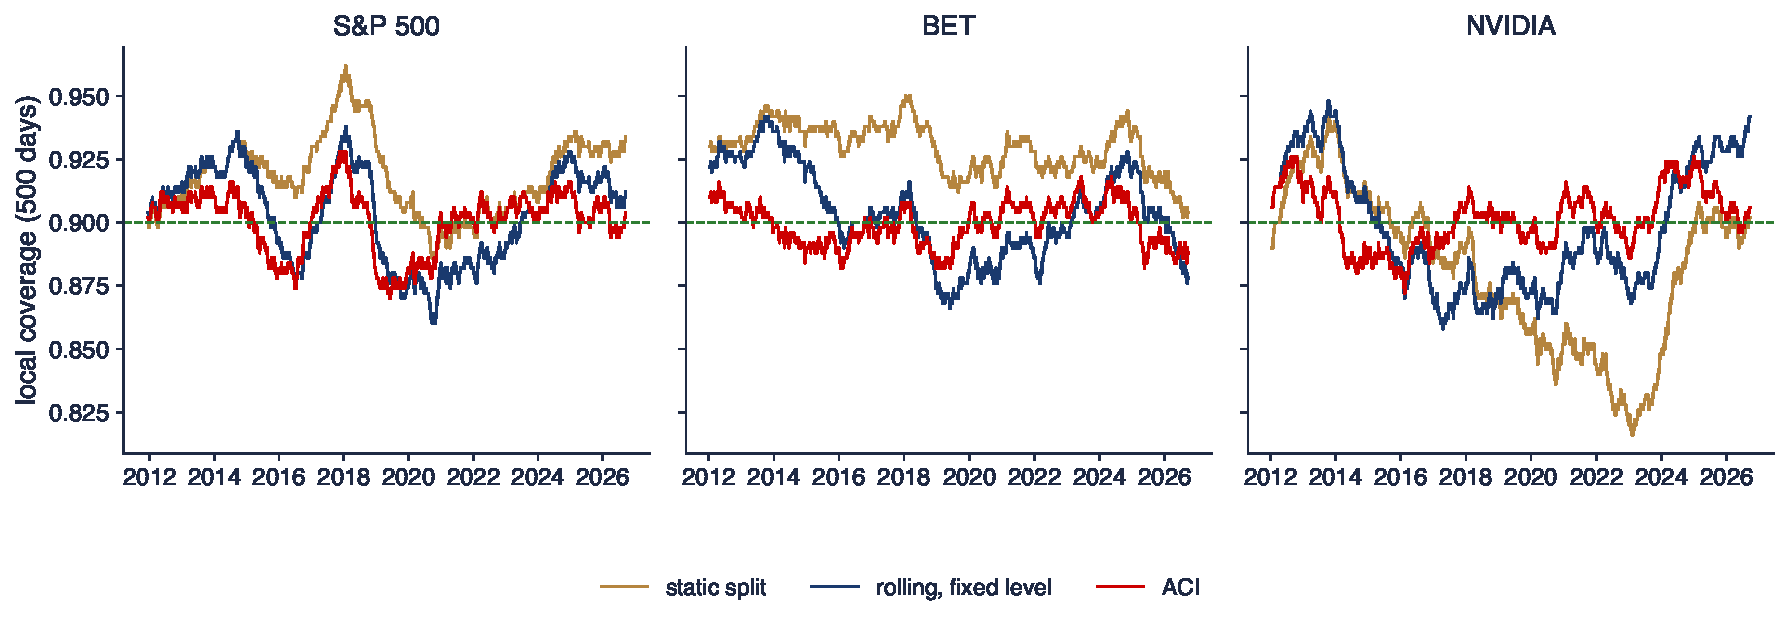
\includegraphics[width=0.97\textwidth,height=0.46\textheight,keepaspectratio]{ats_ch13_aci.pdf}
\end{center}
\vspace{-0.25cm}
\begin{itemize}
    \item Design of \refGC: $V_t = r_t^2$, $\hat\sigma_t^2$ from a GARCH(1,1) fitted on the previous 1250 days, score $|V_t - \hat\sigma_t^2|/\hat\sigma_t^2$, $\alpha = 0.1$, $\gamma = 0.005$; local coverage over 500 days; evaluation from 15 December 2009
\end{itemize}
\quantlet{ATS\_ch13\_conformal\_time}{\qlurl{ATS_ch13_conformal_time}}
\end{frame}

\begin{frame}{Interpreting ACI on volatility}
\itemsize{\small}
\begin{itemize}
    \item Overall coverage, S\&P 500: static 0.918, rolling 0.903, ACI 0.901; BET: 0.928, 0.903, 0.899; NVIDIA: 0.882, 0.900, 0.901
    \item Local coverage of the static method ranges from 0.884 to 0.962 (S\&P 500); ACI stays within 0.870 -- 0.928
    \item Christoffersen conditional coverage of the misses (S\&P 500): static $p$ $<$ 0.001, ACI $p$ = 0.968: a calibration fixed on 2005--2009 is too wide afterwards; updating restores both the frequency and the independence of misses
\end{itemize}
\end{frame}

\begin{frame}{The step size of ACI}
\itemsize{\footnotesize}
\begin{center}
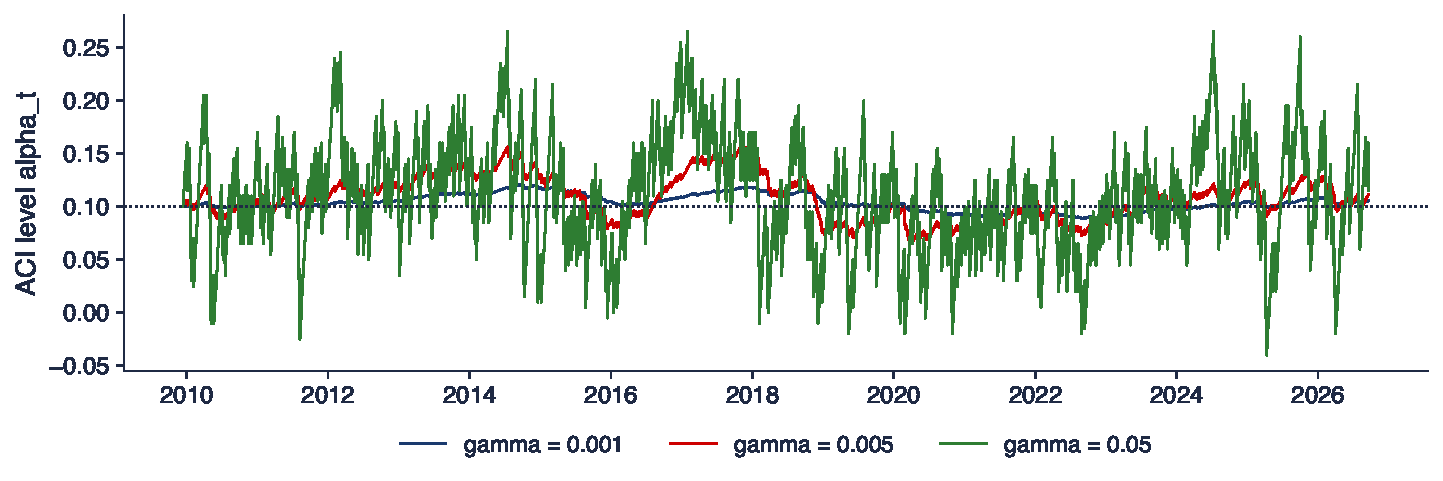
\includegraphics[width=0.97\textwidth,height=0.46\textheight,keepaspectratio]{ats_ch13_aci_gamma.pdf}
\end{center}
\vspace{-0.25cm}
\begin{itemize}
    \item S\&P 500 scores of the previous chart: the level $\alpha_t$ for $\gamma = 0.001$, 0.005 and 0.05
\end{itemize}
\quantlet{ATS\_ch13\_conformal\_time}{\qlurl{ATS_ch13_conformal_time}}
\end{frame}

\begin{frame}{Interpreting the step size}
\itemsize{\small}
\begin{itemize}
    \item Miss rates 0.0987, 0.0994, 0.0999 against the bounds 0.2138, 0.0430, 0.0045 ($T = 4214$): the theorem holds with room to spare
    \item Large $\gamma$: $\alpha_t$ ranges \ensuremath{-}0.04 -- 0.27, infinite intervals on 1.6\% of days; small $\gamma$: slow reaction, long runs of misses after a shock
    \item $\gamma$ trades adaptivity against stability: tune it on a past window, or let DtACI aggregate several values
\end{itemize}
\end{frame}

\begin{frame}{Conformal PID control}
\itemsize{\small}
\begin{itemize}
    \item \refACT: \textbf{quantile tracking} (P): $q_{t+1} = q_t + \eta(\mathrm{err}_t - \alpha)$, i.e.\ online gradient descent on the pinball loss of the score
    \begin{itemize}
        \item \textbf{Proposition}: if $S_t \in [0, B]$, then $\big|\frac1T\sum_t(\mathrm{err}_t - \alpha)\big| \le (B + \eta)/(\eta T)$: the threshold moves on the scale of the scores, not of $\alpha$
    \end{itemize}
    \item \textbf{Integrator} (I): add $r_t\big(\sum_{i \le t}(\mathrm{err}_i - \alpha)\big)$, $r_t(x) = K_I\tan\big(x\log t/(tC_{\mathrm{sat}})\big)$: reacts to accumulated coverage error, saturates to keep the guarantee
    \item \textbf{Scorecaster} (D-like): a model that forecasts the next score from its past (seasonality, trends in the errors) and is added to the threshold
    \item ACI is the special case that tracks the level instead of the quantile; PID borrows its vocabulary from control engineering: proportional, integral, derivative
\end{itemize}
\end{frame}

\begin{frame}{Online methods on Romanian load}
\itemsize{\footnotesize}
\begin{center}
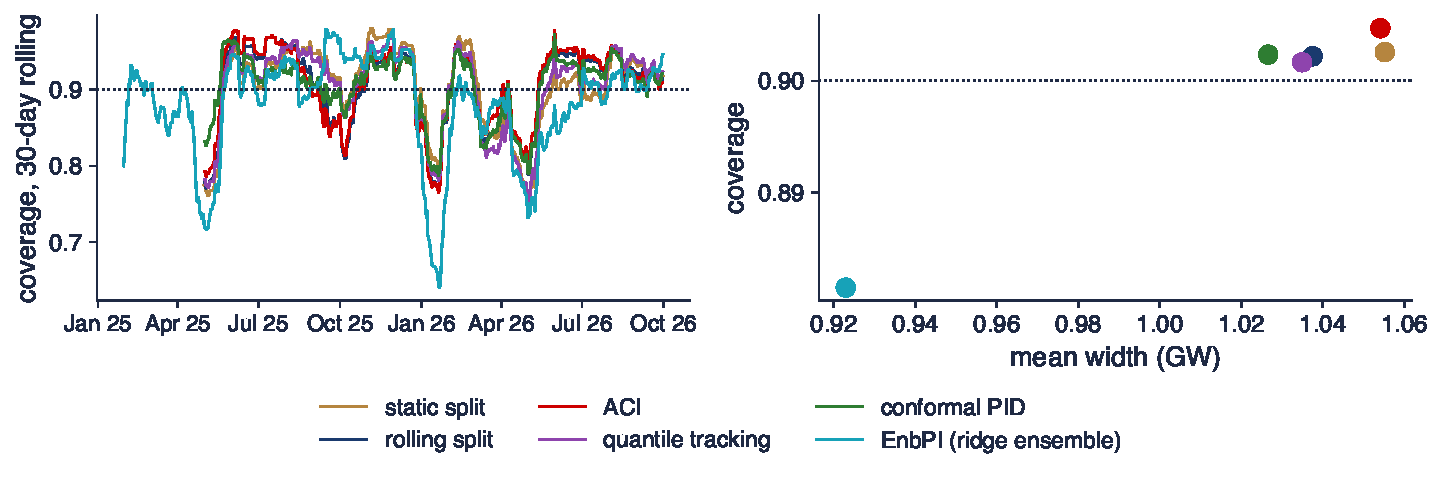
\includegraphics[width=0.97\textwidth,height=0.48\textheight,keepaspectratio]{ats_ch13_pid.pdf}
\end{center}
\vspace{-0.25cm}
\begin{itemize}
    \item 90\% day-ahead intervals around the Chronos-Bolt median, one score stream per hour (24 streams), calibration window 91 days; EnbPI on the expert ARX regressors (ridge, 20 block-bootstrap models); evaluation from 2 April 2025
\end{itemize}
\quantlet{ATS\_ch13\_conformal\_time}{\qlurl{ATS_ch13_conformal_time}}
\end{frame}

\begin{frame}{Interpreting the online methods}
\itemsize{\small}
\begin{itemize}
    \item Coverage: static 0.903, rolling 0.902, ACI 0.905, quantile tracking 0.902, PID 0.902, EnbPI 0.881
    \item Mean width (GW): 1.06, 1.04, 1.05, 1.03, 1.03, 0.92; worst 30-day coverage: static 0.747, PID 0.787
    \item Over the whole period every method except EnbPI is close to 90\%; the differences are in the dips after seasonal transitions and in width, where PID is best on both counts
    \item EnbPI centres the band on its own ridge ensemble, less accurate than the base forecast: narrower intervals, lower coverage
\end{itemize}
\end{frame}

\begin{frame}{Coverage diagnostics}
\itemsize{\small}
\begin{itemize}
    \item \textbf{Unconditional}: miss rate and Kupiec \refKup; \textbf{independence} of misses: Christoffersen \refChr{} (\atschlink{https://danpele.github.io/Advanced-Time-Series/EN/Courses/chapter9_var_es_backtesting.pdf}{Chapter 9})
    \begin{itemize}
        \item regression check in the spirit of the DQ test \refEM: regress $\mathrm{err}_t - \alpha$ on lagged misses and on the predicted width
    \end{itemize}
    \item \textbf{Local}: rolling coverage; coverage by bins of a variable known at the origin (predicted volatility, hour, regime): the empirical counterpart of conditional coverage
    \item \textbf{Sharpness}: mean width and the interval score $W + \frac{2}{\alpha}(\ell - y)\mathbf 1\{y < \ell\} + \frac{2}{\alpha}(y - u)\mathbf 1\{y > u\}$ \refWin, \refGR, a proper score for central intervals
    \item Report all three: a method that is valid but twice as wide is not a better method
\end{itemize}
\end{frame}

\begin{frame}{Coverage by volatility regime}
\itemsize{\footnotesize}
\begin{center}
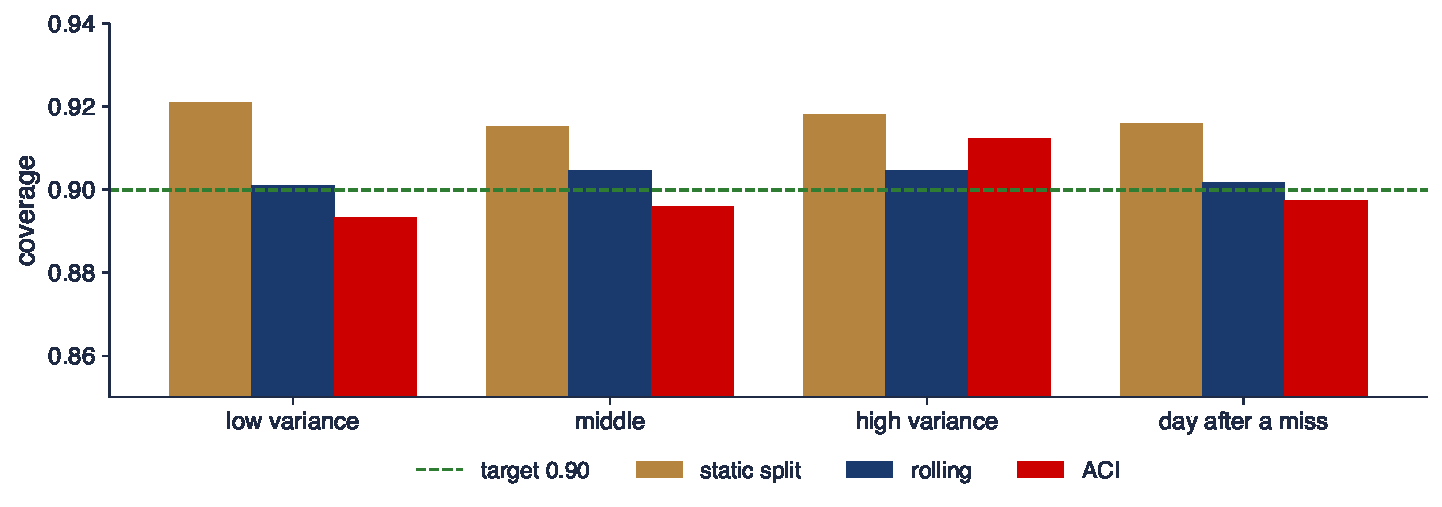
\includegraphics[width=0.97\textwidth,height=0.46\textheight,keepaspectratio]{ats_ch13_condcov.pdf}
\end{center}
\vspace{-0.25cm}
\begin{itemize}
    \item S\&P 500, 90\% volatility intervals of the ACI chart: coverage by tercile of the GARCH variance forecast and on the day after a miss
\end{itemize}
\quantlet{ATS\_ch13\_conformal\_time}{\qlurl{ATS_ch13_conformal_time}}
\end{frame}

\begin{frame}{Interpreting conditional coverage}
\itemsize{\small}
\begin{itemize}
    \item Static: 0.921 (low variance), 0.918 (high), 0.916 after a miss; ACI: 0.893, 0.912, 0.897
    \item Coverage is almost flat across volatility terciles and after a miss, for every method: dividing by the GARCH variance makes the score close to pivotal
    \item Contrast: with the raw score $|r_t|$ (Seminar 13, B3) misses cluster in turbulent years whatever the calibration; conditional coverage is a property of the score, not of the conformal step
\end{itemize}
\end{frame}

\begin{frame}{Recap: conformal methods for time series}
\itemsize{\small}
\begin{itemize}
    \item Weighted conformal: a coverage bound in total variation; geometric weights adapt to drift
    \item EnbPI: bootstrap ensembles and a sliding residual window, asymptotic validity under mixing
    \item ACI and PID: feedback on misses gives long-run coverage for any sequence; conditional coverage must still be tested
\end{itemize}
\end{frame}


%=============================================================================
\section{Calibrating foundation-model intervals}
%=============================================================================

\begin{frame}{The need to calibrate foundation-model quantiles}
\itemsize{\small}
\begin{itemize}
    \item Pretrained quantiles are calibrated on the corpus distribution, not on your series: miscalibration is the default, in either direction
    \item Most models output only 10\%--90\%: a 95\% interval or VaR 1\% requires extrapolation beyond the trained levels
    \item Recipe: online CQR on the model's own band, score $S_t = \max\{\hat q_{0.1,t} - y_t, y_t - \hat q_{0.9,t}\}$; ACI chooses the threshold for any target level ($80\%$ or $95\%$)
    \begin{itemize}
        \item one-sided version for VaR: $S_t = \hat q_{0.1,t} - y_t$, threshold at level $\alpha$; the VaR is $-(\hat q_{0.1,t} - q_t)$
    \end{itemize}
    \item Further reading on conformal VaR recalibration of foundation models: \refCO; \refTV
\end{itemize}
\end{frame}

\begin{frame}{Raw and conformal coverage of foundation models}
\itemsize{\footnotesize}
\begin{center}
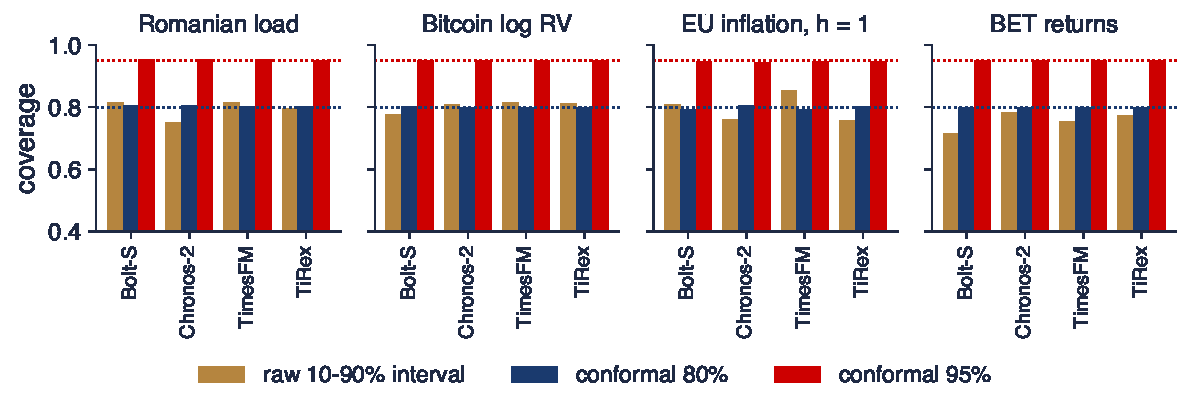
\includegraphics[width=0.97\textwidth,height=0.48\textheight,keepaspectratio]{ats_ch13_fm_calib.pdf}
\end{center}
\vspace{-0.25cm}
\begin{itemize}
    \item Coverage of the raw 10--90\% band and of the online-CQR 80\% and 95\% intervals (ACI, window 250, $\gamma = 0.005$): Romanian load (24 hourly streams), Bitcoin log RV, EU inflation at $h = 1$ (27 streams), BET daily returns
\end{itemize}
\quantlet{ATS\_ch13\_calibration}{\qlurl{ATS_ch13_calibration}}
\end{frame}

\begin{frame}{Interpreting the calibration}
\itemsize{\small}
\begin{itemize}
    \item Raw 80\% bands: load 75--81\%, Bitcoin 77--81\%, inflation 76--85\%, BET returns 72--78\% across the four models
    \item After online CQR: 80\% intervals cover 79--81\%, 95\% intervals 94.5--95.4\% in every task
    \item Raw bands miss in both directions (too narrow: Chronos-2 on load; too wide: TimesFM on inflation); the conformal step widens or narrows them, with a mean width between 0.90 and 1.24 times the raw width, and reaches 95\% from models that output only deciles
\end{itemize}
\end{frame}

\begin{frame}{Value at Risk from foundation models}
\itemsize{\footnotesize}
\begin{center}
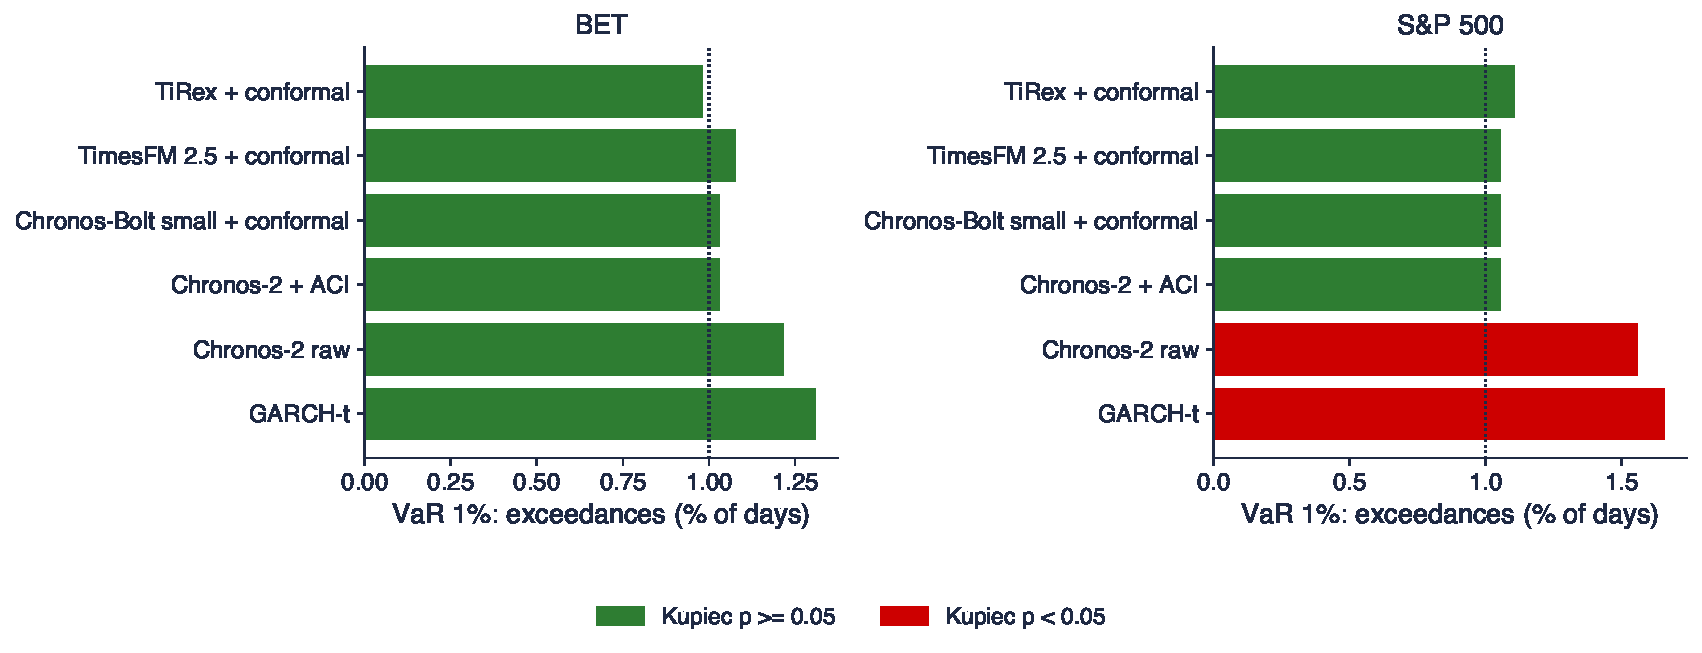
\includegraphics[width=0.97\textwidth,height=0.48\textheight,keepaspectratio]{ats_ch13_fm_var.pdf}
\end{center}
\vspace{-0.25cm}
\begin{itemize}
    \item VaR 1\% exceedances, BET and S\&P 500 from 28 December 2017 (2\,175 days): GARCH-$t$ (rolling 1000 days, \atschlink{https://danpele.github.io/Advanced-Time-Series/EN/Courses/chapter9_var_es_backtesting.pdf}{Chapter 9}), Chronos-2 raw and with ACI, deciles of the other models extended by a one-sided conformal shift
\end{itemize}
\quantlet{ATS\_ch13\_calibration}{\qlurl{ATS_ch13_calibration}}
\end{frame}

\begin{frame}{Interpreting the VaR backtest}
\itemsize{\small}
\begin{itemize}
    \item BET, VaR 1\%: GARCH-$t$ 1.31\% (Kupiec $p$ = 0.170), Chronos-2 raw 1.22\% ($p$ = 0.331), Chronos-2 + ACI 1.03\% ($p$ = 0.893), TimesFM + conformal 1.08\%
    \item S\&P 500: GARCH-$t$ 1.66\% (Kupiec $p$ = 0.007), Chronos-2 raw 1.56\% ($p$ = 0.021), + ACI 1.06\% ($p$ = 0.802, Christoffersen $p$ = 0.454)
    \item Calibration fixes the exceedance rate of every model; it does not add tail information: the conformally extended deciles have a larger quantile loss than GARCH-$t$ (BET, Chronos-Bolt: DM $t = 2.70$), while Chronos-2, trained on 1\% quantiles, does not ($t = 0.10$)
\end{itemize}
\end{frame}

\begin{frame}{Recap: calibration}
\itemsize{\small}
\begin{itemize}
    \item Treat foundation-model quantiles as scores to be calibrated, not as probabilities
    \item Online CQR with ACI gives target coverage at any level, including beyond the trained quantiles
    \item Backtest calibrated VaR as in \atschlink{https://danpele.github.io/Advanced-Time-Series/EN/Courses/chapter9_var_es_backtesting.pdf}{Chapter 9}: frequency, independence and loss
\end{itemize}
\end{frame}


%=============================================================================
\section{AI for scientific discovery}
%=============================================================================

\begin{frame}{An open question}
\itemsize{\small}
\begin{itemize}
    \item Do time-series foundation models beat domain-specific econometric models on Central and Eastern European data after their release dates, once multiplicity is accounted for?
    \begin{itemize}
        \item formal: $H_0$: equal expected loss (pooled over pre-registered series) of the best foundation model and the best domain model, in a window that starts after every model release
        \item falsified by a pooled DM test at 5\% and an MCS that excludes one side, on series and horizons fixed before the data arrive
    \end{itemize}
    \item Why it matters: central banks and grid operators consider replacing tuned models by zero-shot ones; published wins often come from a favourable choice of series
    \begin{itemize}
        \item literature to start from: \refAks, \refShc, \refMey, \refPE, \refBri
    \end{itemize}
\end{itemize}
\end{frame}

\begin{frame}{The discovery loop with an AI assistant}
\itemsize{\footnotesize}
\begin{itemize}
    \item An AI assistant (an LLM such as Claude, ChatGPT, Gemini or Copilot) speeds up each step; Semantic Scholar and Elicit help with the literature
    \begin{itemize}
        \item \textbf{literature}: \aiprompt{List peer-reviewed or arXiv papers since 2024 that evaluate time-series foundation models only after their release dates; give arXiv IDs or DOIs.} Then check every identifier
        \item \textbf{hypothesis}: \aiprompt{Write a pre-registration: series, origins, horizons, losses, baselines, the pooled test and the MCS level.}
        \item \textbf{code and replication}: ask for a wrapper that returns quantiles at fixed levels for each model; replicate a known number first (the Chronos-Bolt quantile range, our load MAE)
        \item \textbf{critique}: \aiprompt{Act as a hostile referee: list every way this benchmark could favour the foundation models.}
    \end{itemize}
    \item Report: what was asked, what was kept, what was rejected (AI\_USE.md, AI\_ERRORS.md)
\end{itemize}
\end{frame}

\begin{frame}{What the human checks}
\itemsize{\small}
\begin{itemize}
    \item Every reference exists and says what is claimed (arXiv ID or DOI resolves, the title matches, the result is in the paper)
    \item Release dates and training cutoffs of every model, from the model cards, against the start of the evaluation window
    \item Quantile levels actually produced by each model (a request for 1\% may silently return 10\%)
    \item Baselines tuned with the same care; the context available to every model is the same
    \item Multiplicity: number of series, horizons and models tested; the pooled test and adjusted $p$-values reported
\end{itemize}
\end{frame}

\begin{frame}{Mini-case: how much can the choice of benchmark change the verdict?}
\itemsize{\footnotesize}
\begin{center}
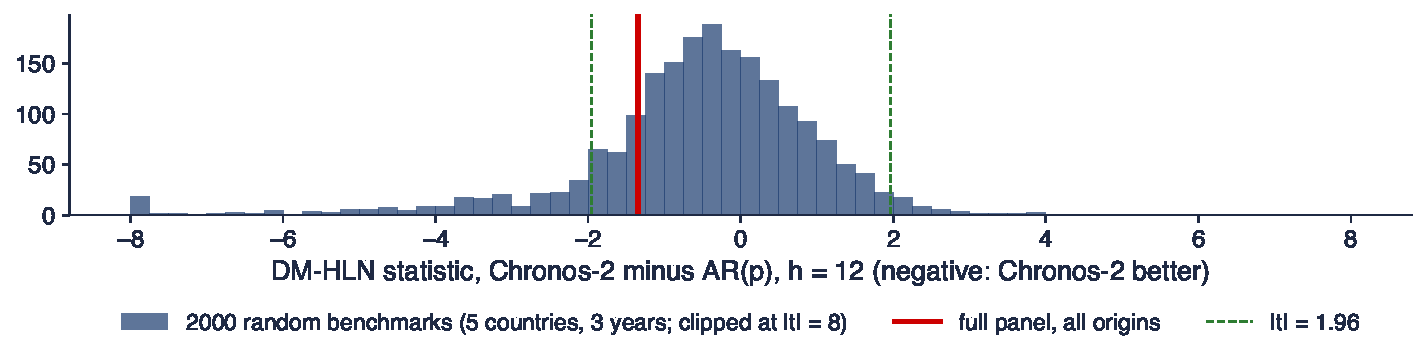
\includegraphics[width=0.97\textwidth,height=0.4\textheight,keepaspectratio]{ats_ch13_ai_case.pdf}
\end{center}
\vspace{-0.25cm}
\begin{itemize}
    \item DM--HLN statistics of Chronos-2 against AR($p$) at $h = 12$ on 2000 random benchmarks of 5 EU countries and 3 years of origins, and on the full panel
    \item 11.2\% of the random benchmarks declare Chronos-2 significantly better and 2.1\% significantly worse; the full panel gives $t = \ensuremath{-}1.35$ ($p$ = 0.180). An AI summary of one such paper as evidence for (or against) foundation models is wrong; only the pre-registered panel answers
\end{itemize}
\quantlet{ATS\_ch13\_benchmark}{\qlurl{ATS_ch13_benchmark}}
\end{frame}

\begin{frame}{Project idea}
\itemsize{\small}
\begin{itemize}
    \item \textbf{A pre-registered, post-release benchmark of foundation models for CEE macro and risk, with conformal calibration}
    \begin{itemize}
        \item replicate: the zero-shot protocol of \refAns{} (WQL, MASE, geometric means) and the ACI volatility design of \refGC{} on our data
        \item extend: Romanian, Polish, Hungarian and Czech inflation, load and stock indices; covariates in context (energy prices, calendars); online CQR to 95\% and VaR 1\%; pooled tests with Holm and BH
        \item pre-register: series, origins after 1 November 2025, horizons, losses, baselines and the decision rule; forecasts for the next months written down before the data arrive
    \end{itemize}
    \item Deliverables follow the course rules: repository, report, AI\_USE.md, AI\_ERRORS.md, oral defence
\end{itemize}
\end{frame}


%=============================================================================
\section{Wrap-up}
%=============================================================================

\begin{frame}{Key takeaways}
\itemsize{\small}
\begin{itemize}
    \item Foundation models amortise estimation over a corpus; design choices (scaling, patches, quantile range) set what they can and cannot forecast
    \item On our data the best zero-shot model is competitive with domain models; gains depend on the task and do not survive cherry-picking
    \item Evaluate after the release, pool across series, correct for multiplicity
    \item Conformal prediction gives finite-sample marginal coverage under exchangeability; under dependence, weights, ensembles and feedback restore long-run coverage
    \item Conditional coverage is impossible in general: diagnose it with Christoffersen tests and coverage by regime
\end{itemize}
\end{frame}

\begin{frame}{Self-assessment}
\itemsize{\small}
\begin{columns}[T]
\begin{column}{0.56\textwidth}
\begin{block}{Questions}
\begin{itemize}
    \item Why can Chronos not forecast a value above $15s$?
    \item Why does a stationary AR(1) violate exchangeability?
    \item What is the law of the coverage of split conformal given the calibration set?
    \item Which quantity stays bounded in the proof of the ACI theorem?
    \item Why is a post-release window necessary in a foundation-model benchmark?
\end{itemize}
\end{block}
\end{column}
\begin{column}{0.40\textwidth}
\begin{block}{Next: \atschlink{https://danpele.github.io/Advanced-Time-Series/EN/Courses/chapter14_causal_inference_time_series.pdf}{Chapter 14}}
\begin{itemize}
    \item Causal inference for time series
    \item Granger and structural causality, causal discovery, policy evaluation
\end{itemize}
\end{block}
\end{column}
\end{columns}
\end{frame}


%=============================================================================
\section{Appendix}
%=============================================================================

\begin{frame}{Appendix: proof of split conformal coverage}
\hypertarget{atsapp1}{}\atsappback{atssrc1}{Back}
\itemsize{\small}
\begin{itemize}
    \item Condition on the training set, so $\hat\mu$ and $s$ are fixed; exchangeability of $Z_1, \dots, Z_{n+1}$ implies exchangeability of $S_1, \dots, S_{n+1}$
    \item With no ties, the rank $R$ of $S_{n+1}$ among $S_1, \dots, S_{n+1}$ is uniform on $\{1, \dots, n + 1\}$ (every ordering is equally likely)
    \item $S_{n+1} \le S_{(k)}$ (order statistic of the first $n$) $\iff R \le k$; so $\Pr\{Y_{n+1} \in \hat C\} = k/(n + 1)$
    \item $k = \lceil (n + 1)(1 - \alpha)\rceil$ gives $1 - \alpha \le k/(n + 1) < 1 - \alpha + 1/(n + 1)$; ties only increase coverage
    \item Given the calibration set, coverage is $F(S_{(k)})$ with $F$ the score distribution; $F(S_i)$ are i.i.d.\ uniform, so $F(S_{(k)}) \sim$ Beta($k$, $n + 1 - k$)
\end{itemize}
\end{frame}

\begin{frame}{Appendix: the two online guarantees}
\hypertarget{atsapp2}{}\atsappback{atssrc1}{Back}
\itemsize{\small}
\begin{itemize}
    \item \textbf{ACI}: if $\alpha_t < 0$ then $q_t = +\infty$ and $\mathrm{err}_t = 0$, so $\alpha_{t+1} = \alpha_t + \gamma\alpha > \alpha_t$; if $\alpha_t > 1$, $\mathrm{err}_t = 1$ and $\alpha_t$ falls
    \begin{itemize}
        \item hence $\alpha_t \in [-\gamma, 1 + \gamma]$ for all $t$; summing the updates, $\gamma\big|\sum_{t \le T}(\alpha - \mathrm{err}_t)\big| = |\alpha_{T+1} - \alpha_1| \le \max\{\alpha_1, 1 - \alpha_1\} + \gamma$
    \end{itemize}
    \item \textbf{Quantile tracking}: if $q_t > B$ then $\mathrm{err}_t = 0$ and $q_t$ falls by $\eta\alpha$; if $q_t < 0$ then $\mathrm{err}_t = 1$ and $q_t$ rises
    \begin{itemize}
        \item hence $q_t \in [-\eta, B + \eta]$ (starting inside); $\eta\sum_{t \le T}(\mathrm{err}_t - \alpha) = q_{T+1} - q_1$, so the average gap is at most $(B + \eta)/(\eta T)$
    \end{itemize}
    \item Neither proof uses any probability: the guarantees hold for every sequence, which is why they say nothing about conditional coverage
\end{itemize}
\end{frame}


%=============================================================================
\section{References}
%=============================================================================

\begin{frame}{References (1/6)}
\itemsize{\tiny}
\begin{itemize}
    \item Aksu, T., Woo, G., Liu, J., Liu, X., Liu, C., Savarese, S., Xiong, C., \& Sahoo, D. (2024). GIFT-Eval: A benchmark for general time series forecasting model evaluation. \textit{arXiv:2410.10393}. \href{https://arxiv.org/abs/2410.10393}{arXiv:2410.10393}
    \item Angelopoulos, A. N., \& Bates, S. (2023). Conformal prediction: A gentle introduction. \textit{Foundations and Trends in Machine Learning}, 16(4), 494--591. \href{https://doi.org/10.1561/2200000101}{doi:10.1561/2200000101}
    \item Angelopoulos, A. N., Candès, E. J., \& Tibshirani, R. J. (2023). Conformal PID control for time series prediction. \textit{Advances in Neural Information Processing Systems 36}; \textit{arXiv:2307.16895}. \href{https://arxiv.org/abs/2307.16895}{arXiv:2307.16895}
    \item Ansari, A. F., Shchur, O., Küken, J., Auer, A., Han, B., Mercado, P., et al.\ (2025). Chronos-2: From univariate to universal forecasting. \textit{arXiv:2510.15821}. \href{https://arxiv.org/abs/2510.15821}{arXiv:2510.15821}
    \item Ansari, A. F., Stella, L., Turkmen, C., Zhang, X., Mercado, P., Shen, H., et al.\ (2024). Chronos: Learning the language of time series. \textit{Transactions on Machine Learning Research}; \textit{arXiv:2403.07815}. \href{https://arxiv.org/abs/2403.07815}{arXiv:2403.07815}
    \item Auer, A., Podest, P., Klotz, D., Böck, S., Klambauer, G., \& Hochreiter, S. (2025). TiRex: Zero-shot forecasting across long and short horizons with enhanced in-context learning. \textit{Advances in Neural Information Processing Systems}; \textit{arXiv:2505.23719}. \href{https://arxiv.org/abs/2505.23719}{arXiv:2505.23719}
    \item Barber, R. F., Candès, E. J., Ramdas, A., \& Tibshirani, R. J. (2023). Conformal prediction beyond exchangeability. \textit{The Annals of Statistics}, 51(2), 816--845. \href{https://doi.org/10.1214/23-AOS2276}{doi:10.1214/23-AOS2276}
    \item Benjamini, Y., \& Hochberg, Y. (1995). Controlling the false discovery rate: A practical and powerful approach to multiple testing. \textit{Journal of the Royal Statistical Society: Series B}, 57(1), 289--300. \href{https://doi.org/10.1111/j.2517-6161.1995.tb02031.x}{doi:10.1111/j.2517-6161.1995.tb02031.x}
    \item Bollerslev, T. (1986). Generalized autoregressive conditional heteroskedasticity. \textit{Journal of Econometrics}, 31(3), 307--327. \href{https://doi.org/10.1016/0304-4076(86)90063-1}{doi:10.1016/0304-4076(86)90063-1}
    \item Bommasani, R., Hudson, D. A., Adeli, E., Altman, R., Arora, S., et al.\ (2021). On the opportunities and risks of foundation models. \textit{arXiv:2108.07258}. \href{https://arxiv.org/abs/2108.07258}{arXiv:2108.07258}
    \item Brini, A. (2026). Forecasting realized volatility with time series foundation models: A comparison with econometric benchmarks. \textit{arXiv:2607.05291}. \href{https://arxiv.org/abs/2607.05291}{arXiv:2607.05291}
    \item Chernozhukov, V., Wüthrich, K., \& Zhu, Y. (2018). Exact and robust conformal inference methods for predictive machine learning with dependent data. \textit{Proceedings of the 31st Conference on Learning Theory (COLT)}; \textit{arXiv:1802.06300}. \href{https://arxiv.org/abs/1802.06300}{arXiv:1802.06300}
    \item Christoffersen, P. F. (1998). Evaluating interval forecasts. \textit{International Economic Review}, 39(4), 841--862. \href{https://doi.org/10.2307/2527341}{doi:10.2307/2527341}
    \item Cohen, B., Khwaja, E., Doubli, Y., Lemaachi, S., Lettieri, C., Masson, C., et al.\ (2025). This time is different: An observability perspective on time series foundation models. \textit{arXiv:2505.14766}. \href{https://arxiv.org/abs/2505.14766}{arXiv:2505.14766}
\end{itemize}
\end{frame}

\begin{frame}{References (2/6)}
\itemsize{\tiny}
\begin{itemize}
    \item Corsi, F. (2009). A simple approximate long-memory model of realized volatility. \textit{Journal of Financial Econometrics}, 7(2), 174--196. \href{https://doi.org/10.1093/jjfinec/nbp001}{doi:10.1093/jjfinec/nbp001}
    \item Das, A., Kong, W., Sen, R., \& Zhou, Y. (2024). A decoder-only foundation model for time-series forecasting. \textit{Proceedings of the 41st International Conference on Machine Learning (ICML)}; \textit{arXiv:2310.10688}. \href{https://arxiv.org/abs/2310.10688}{arXiv:2310.10688}
    \item Demšar, J. (2006). Statistical comparisons of classifiers over multiple data sets. \textit{Journal of Machine Learning Research}, 7, 1--30. \href{https://jmlr.org/papers/v7/demsar06a.html}{jmlr.org}
    \item Diebold, F. X., \& Mariano, R. S. (1995). Comparing predictive accuracy. \textit{Journal of Business \& Economic Statistics}, 13(3), 253--263. \href{https://doi.org/10.1080/07350015.1995.10524599}{doi:10.1080/07350015.1995.10524599}
    \item Edwards, T. D. P., Alvey, J., Alsing, J., Nguyen, N. H., \& Wandelt, B. D. (2024). Scaling-laws for large time-series models. \textit{arXiv:2405.13867}. \href{https://arxiv.org/abs/2405.13867}{arXiv:2405.13867}
    \item Engle, R. F., \& Manganelli, S. (2004). CAViaR: Conditional autoregressive value at risk by regression quantiles. \textit{Journal of Business \& Economic Statistics}, 22(4), 367--381. \href{https://doi.org/10.1198/073500104000000370}{doi:10.1198/073500104000000370}
    \item Fleming, P. J., \& Wallace, J. J. (1986). How not to lie with statistics: The correct way to summarize benchmark results. \textit{Communications of the ACM}, 29(3), 218--221. \href{https://doi.org/10.1145/5666.5673}{doi:10.1145/5666.5673}
    \item Foygel Barber, R., Candès, E. J., Ramdas, A., \& Tibshirani, R. J. (2021). The limits of distribution-free conditional predictive inference. \textit{Information and Inference: A Journal of the IMA}, 10(2), 455--482. \href{https://doi.org/10.1093/imaiai/iaaa017}{doi:10.1093/imaiai/iaaa017}
    \item Garza, A., Challu, C., \& Mergenthaler-Canseco, M. (2023). TimeGPT-1. \textit{arXiv:2310.03589}. \href{https://arxiv.org/abs/2310.03589}{arXiv:2310.03589}
    \item Garza, A., Rosillo, R., Mendoza-Smith, R., Salinas, D., Williams, A. R., Ashok, A., Goswami, M., et al.\ (2026). Impermanent: A live benchmark for temporal generalization in time series forecasting. \textit{arXiv:2603.08707}. \href{https://arxiv.org/abs/2603.08707}{arXiv:2603.08707}
    \item Giacomini, R., \& White, H. (2006). Tests of conditional predictive ability. \textit{Econometrica}, 74(6), 1545--1578. \href{https://doi.org/10.1111/j.1468-0262.2006.00718.x}{doi:10.1111/j.1468-0262.2006.00718.x}
    \item Gibbs, I., \& Candès, E. (2021). Adaptive conformal inference under distribution shift. \textit{Advances in Neural Information Processing Systems 34}; \textit{arXiv:2106.00170}. \href{https://arxiv.org/abs/2106.00170}{arXiv:2106.00170}
    \item Gibbs, I., \& Candès, E. J. (2024). Conformal inference for online prediction with arbitrary distribution shifts. \textit{Journal of Machine Learning Research}, 25(162), 1--36. \href{https://jmlr.org/papers/v25/22-1218.html}{jmlr.org}
    \item Gneiting, T., \& Raftery, A. E. (2007). Strictly proper scoring rules, prediction, and estimation. \textit{Journal of the American Statistical Association}, 102(477), 359--378. \href{https://doi.org/10.1198/016214506000001437}{doi:10.1198/016214506000001437}
\end{itemize}
\end{frame}

\begin{frame}{References (3/6)}
\itemsize{\tiny}
\begin{itemize}
    \item Goel, A., Pasricha, P., Magris, M., \& Kanniainen, J. (2025). Foundation time-series AI model for realized volatility forecasting. \textit{arXiv:2505.11163}. \href{https://arxiv.org/abs/2505.11163}{arXiv:2505.11163}
    \item Goswami, M., Szafer, K., Choudhry, A., Cai, Y., Li, S., \& Dubrawski, A. (2024). MOMENT: A family of open time-series foundation models. \textit{Proceedings of the 41st International Conference on Machine Learning (ICML)}; \textit{arXiv:2402.03885}. \href{https://arxiv.org/abs/2402.03885}{arXiv:2402.03885}
    \item Gruver, N., Finzi, M., Qiu, S., \& Wilson, A. G. (2023). Large language models are zero-shot time series forecasters. \textit{Advances in Neural Information Processing Systems 36}; \textit{arXiv:2310.07820}. \href{https://arxiv.org/abs/2310.07820}{arXiv:2310.07820}
    \item Hansen, P. R., Lunde, A., \& Nason, J. M. (2011). The model confidence set. \textit{Econometrica}, 79(2), 453--497. \href{https://doi.org/10.3982/ECTA5771}{doi:10.3982/ECTA5771}
    \item Harvey, D., Leybourne, S., \& Newbold, P. (1997). Testing the equality of prediction mean squared errors. \textit{International Journal of Forecasting}, 13(2), 281--291. \href{https://doi.org/10.1016/S0169-2070(96)00719-4}{doi:10.1016/S0169-2070(96)00719-4}
    \item Heber, G., Lunde, A., Shephard, N., \& Sheppard, K. (2009). \textit{Oxford-Man Institute's realized library}, version 0.3. Oxford-Man Institute, University of Oxford. \href{https://web.archive.org/web/20220301022212/https://realized.oxford-man.ox.ac.uk/}{web.archive.org}
    \item Hewamalage, H., Ackermann, K., \& Bergmeir, C. (2023). Forecast evaluation for data scientists: Common pitfalls and best practices. \textit{Data Mining and Knowledge Discovery}, 37, 788--832. \href{https://doi.org/10.1007/s10618-022-00894-5}{doi:10.1007/s10618-022-00894-5}
    \item Hoffmann, J., Borgeaud, S., Mensch, A., Buchatskaya, E., et al.\ (2022). Training compute-optimal large language models. \textit{arXiv:2203.15556}. \href{https://arxiv.org/abs/2203.15556}{arXiv:2203.15556}
    \item Holm, S. (1979). A simple sequentially rejective multiple test procedure. \textit{Scandinavian Journal of Statistics}, 6(2), 65--70. \href{https://www.jstor.org/stable/4615733}{jstor.org}
    \item Hong, T., \& Fan, S. (2016). Probabilistic electric load forecasting: A tutorial review. \textit{International Journal of Forecasting}, 32(3), 914--938. \href{https://doi.org/10.1016/j.ijforecast.2015.11.011}{doi:10.1016/j.ijforecast.2015.11.011}
    \item Hyndman, R. J., \& Koehler, A. B. (2006). Another look at measures of forecast accuracy. \textit{International Journal of Forecasting}, 22(4), 679--688. \href{https://doi.org/10.1016/j.ijforecast.2006.03.001}{doi:10.1016/j.ijforecast.2006.03.001}
    \item Hyndman, R. J., Koehler, A. B., Snyder, R. D., \& Grose, S. (2002). A state space framework for automatic forecasting using exponential smoothing methods. \textit{International Journal of Forecasting}, 18(3), 439--454. \href{https://doi.org/10.1016/S0169-2070(01)00110-8}{doi:10.1016/S0169-2070(01)00110-8}
    \item Jin, M., Wang, S., Ma, L., Chu, Z., Zhang, J. Y., Shi, X., et al.\ (2024). Time-LLM: Time series forecasting by reprogramming large language models. \textit{International Conference on Learning Representations (ICLR)}; \textit{arXiv:2310.01728}. \href{https://arxiv.org/abs/2310.01728}{arXiv:2310.01728}
    \item Kaplan, J., McCandlish, S., Henighan, T., Brown, T. B., Chess, B., Child, R., et al.\ (2020). Scaling laws for neural language models. \textit{arXiv:2001.08361}. \href{https://arxiv.org/abs/2001.08361}{arXiv:2001.08361}
\end{itemize}
\end{frame}

\begin{frame}{References (4/6)}
\itemsize{\tiny}
\begin{itemize}
    \item Koenker, R., \& Bassett, G. (1978). Regression quantiles. \textit{Econometrica}, 46(1), 33--50. \href{https://doi.org/10.2307/1913643}{doi:10.2307/1913643}
    \item Kupiec, P. H. (1995). Techniques for verifying the accuracy of risk measurement models. \textit{The Journal of Derivatives}, 3(2), 73--84. \href{https://doi.org/10.3905/jod.1995.407942}{doi:10.3905/jod.1995.407942}
    \item Lei, J., G'Sell, M., Rinaldo, A., Tibshirani, R. J., \& Wasserman, L. (2018). Distribution-free predictive inference for regression. \textit{Journal of the American Statistical Association}, 113(523), 1094--1111. \href{https://doi.org/10.1080/01621459.2017.1307116}{doi:10.1080/01621459.2017.1307116}
    \item Lei, J., \& Wasserman, L. (2014). Distribution-free prediction bands for non-parametric regression. \textit{Journal of the Royal Statistical Society: Series B}, 76(1), 71--96. \href{https://doi.org/10.1111/rssb.12021}{doi:10.1111/rssb.12021}
    \item Lim, B., Arık, S. Ö., Loeff, N., \& Pfister, T. (2021). Temporal Fusion Transformers for interpretable multi-horizon time series forecasting. \textit{International Journal of Forecasting}, 37(4), 1748--1764. \href{https://doi.org/10.1016/j.ijforecast.2021.03.012}{doi:10.1016/j.ijforecast.2021.03.012}
    \item Liu, C., Aksu, T., Liu, J., Liu, X., Yan, H., Pham, Q., Savarese, S., et al.\ (2025). Moirai 2.0: When less is more for time series forecasting. \textit{arXiv:2511.11698}. \href{https://arxiv.org/abs/2511.11698}{arXiv:2511.11698}
    \item Lopez-Lira, A., Tang, Y., \& Zhu, M. (2025). The memorization problem: Can we trust LLMs' economic forecasts? \textit{arXiv:2504.14765}. \href{https://arxiv.org/abs/2504.14765}{arXiv:2504.14765}
    \item Makridakis, S., Spiliotis, E., \& Assimakopoulos, V. (2022). M5 accuracy competition: Results, findings, and conclusions. \textit{International Journal of Forecasting}, 38(4), 1346--1364. \href{https://doi.org/10.1016/j.ijforecast.2021.11.013}{doi:10.1016/j.ijforecast.2021.11.013}
    \item Meyer, M., Kaltenpoth, S., Albers, H., Zalipski, K., \& Müller, O. (2025). TS-Arena: A live forecast pre-registration platform. \textit{arXiv:2512.20761}. \href{https://arxiv.org/abs/2512.20761}{arXiv:2512.20761}
    \item Nie, Y., Nguyen, N. H., Sinthong, P., \& Kalagnanam, J. (2023). A time series is worth 64 words: Long-term forecasting with Transformers. \textit{International Conference on Learning Representations (ICLR)}; \textit{arXiv:2211.14730}. \href{https://arxiv.org/abs/2211.14730}{arXiv:2211.14730}
    \item Oliveira, R. I., Orenstein, P., Ramos, T., \& Romano, J. V. (2024). Split conformal prediction and non-exchangeable data. \textit{Journal of Machine Learning Research}, 25; \textit{arXiv:2203.15885}. \href{https://arxiv.org/abs/2203.15885}{arXiv:2203.15885}
    \item Oreshkin, B. N., Carpov, D., Chapados, N., \& Bengio, Y. (2020). N-BEATS: Neural basis expansion analysis for interpretable time series forecasting. \textit{International Conference on Learning Representations (ICLR)}; \textit{arXiv:1905.10437}. \href{https://arxiv.org/abs/1905.10437}{arXiv:1905.10437}
    \item Pan, Z., \& Ezzat, A. A. (2026). Evaluating time series foundation models for electricity price forecasting: Contamination risk, distributional shifts, and covariate dependence. \textit{arXiv:2607.02623}. \href{https://arxiv.org/abs/2607.02623}{arXiv:2607.02623}
    \item Papadopoulos, H., Proedrou, K., Vovk, V., \& Gammerman, A. (2002). Inductive confidence machines for regression. In \textit{Machine Learning: ECML 2002}, Lecture Notes in Computer Science 2430, 345--356. Springer. \href{https://doi.org/10.1007/3-540-36755-1_29}{doi:10.1007/3-540-36755-1\_29}
\end{itemize}
\end{frame}

\begin{frame}{References (5/6)}
\itemsize{\tiny}
\begin{itemize}
    \item Patton, A. J. (2011). Volatility forecast comparison using imperfect volatility proxies. \textit{Journal of Econometrics}, 160(1), 246--256. \href{https://doi.org/10.1016/j.jeconom.2010.03.034}{doi:10.1016/j.jeconom.2010.03.034}
    \item Pele, D. T., et al. Conformal\_Oracle: conformal VaR recalibration for time series foundation models and classical models. GitHub repository (further reading). \href{https://github.com/danpele/Conformal_Oracle}{github.com}
    \item Pele, D. T., et al. TSFM\_VaR\_CEE: benchmarking time-series foundation models for VaR and ES forecasting in Central and Eastern European markets. GitHub repository (further reading). \href{https://github.com/danpele/TSFM_VaR_CEE}{github.com}
    \item Petropoulos, F., Apiletti, D., Assimakopoulos, V., Babai, M. Z., et al.\ (2022). Forecasting: Theory and practice. \textit{International Journal of Forecasting}, 38(3), 705--871. \href{https://doi.org/10.1016/j.ijforecast.2021.11.001}{doi:10.1016/j.ijforecast.2021.11.001}
    \item Rahimikia, E., Ni, H., \& Wang, W. (2025). Re(Visiting) time series foundation models in finance. \textit{arXiv:2511.18578}. \href{https://arxiv.org/abs/2511.18578}{arXiv:2511.18578}
    \item Rasul, K., Ashok, A., Williams, A. R., Ghonia, H., Bhagwatkar, R., Khorasani, A., et al.\ (2023). Lag-Llama: Towards foundation models for probabilistic time series forecasting. \textit{arXiv:2310.08278}. \href{https://arxiv.org/abs/2310.08278}{arXiv:2310.08278}
    \item Romano, Y., Patterson, E., \& Candès, E. (2019). Conformalized quantile regression. \textit{Advances in Neural Information Processing Systems 32}; \textit{arXiv:1905.03222}. \href{https://arxiv.org/abs/1905.03222}{arXiv:1905.03222}
    \item Salinas, D., Flunkert, V., Gasthaus, J., \& Januschowski, T. (2020). DeepAR: Probabilistic forecasting with autoregressive recurrent networks. \textit{International Journal of Forecasting}, 36(3), 1181--1191. \href{https://doi.org/10.1016/j.ijforecast.2019.07.001}{doi:10.1016/j.ijforecast.2019.07.001}
    \item Shchur, O., Ansari, A. F., Turkmen, C., Stella, L., Erickson, N., Guerron, P., et al.\ (2025). fev-bench: A realistic benchmark for time series forecasting. \textit{arXiv:2509.26468}. \href{https://arxiv.org/abs/2509.26468}{arXiv:2509.26468}
    \item Shi, J., Ma, Q., Ma, H., \& Li, L. (2024). Scaling law for time series forecasting. \textit{Advances in Neural Information Processing Systems 37}; \textit{arXiv:2405.15124}. \href{https://arxiv.org/abs/2405.15124}{arXiv:2405.15124}
    \item Tan, M., Merrill, M. A., Gupta, V., Althoff, T., \& Hartvigsen, T. (2024). Are language models actually useful for time series forecasting? \textit{Advances in Neural Information Processing Systems 37}; \textit{arXiv:2406.16964}. \href{https://arxiv.org/abs/2406.16964}{arXiv:2406.16964}
    \item Tibshirani, R. J., Barber, R. F., Candès, E. J., \& Ramdas, A. (2019). Conformal prediction under covariate shift. \textit{Advances in Neural Information Processing Systems 32}; \textit{arXiv:1904.06019}. \href{https://arxiv.org/abs/1904.06019}{arXiv:1904.06019}
    \item Vaswani, A., Shazeer, N., Parmar, N., Uszkoreit, J., Jones, L., Gomez, A. N., Kaiser, Ł., \& Polosukhin, I. (2017). Attention is all you need. \textit{Advances in Neural Information Processing Systems 30}; \textit{arXiv:1706.03762}. \href{https://arxiv.org/abs/1706.03762}{arXiv:1706.03762}
    \item Vovk, V. (2012). Conditional validity of inductive conformal predictors. \textit{Proceedings of the Asian Conference on Machine Learning}, PMLR 25, 475--490. \href{https://proceedings.mlr.press/v25/vovk12.html}{proceedings.mlr.press}
\end{itemize}
\end{frame}

\begin{frame}{References (6/6)}
\itemsize{\tiny}
\begin{itemize}
    \item Vovk, V., Gammerman, A., \& Shafer, G. (2022). \textit{Algorithmic Learning in a Random World} (2nd ed.). Springer. \href{https://doi.org/10.1007/978-3-031-06649-8}{doi:10.1007/978-3-031-06649-8}
    \item Vovk, V., Gammerman, A., \& Shafer, G. (2005). \textit{Algorithmic Learning in a Random World}. Springer. \href{https://doi.org/10.1007/b106715}{doi:10.1007/b106715}
    \item Winkler, R. L. (1972). A decision-theoretic approach to interval estimation. \textit{Journal of the American Statistical Association}, 67(337), 187--191. \href{https://doi.org/10.1080/01621459.1972.10481224}{doi:10.1080/01621459.1972.10481224}
    \item Woo, G., Liu, C., Kumar, A., Xiong, C., Savarese, S., \& Sahoo, D. (2024). Unified training of universal time series forecasting Transformers. \textit{Proceedings of the 41st International Conference on Machine Learning (ICML)}; \textit{arXiv:2402.02592}. \href{https://arxiv.org/abs/2402.02592}{arXiv:2402.02592}
    \item Xu, C., \& Xie, Y. (2023). Conformal prediction for time series. \textit{IEEE Transactions on Pattern Analysis and Machine Intelligence}, 45(10), 11575--11587. \href{https://doi.org/10.1109/TPAMI.2023.3272339}{doi:10.1109/TPAMI.2023.3272339}
    \item Xu, C., \& Xie, Y. (2021). Conformal prediction interval for dynamic time-series. \textit{Proceedings of the 38th International Conference on Machine Learning (ICML)}, PMLR 139, 11559--11569. \href{https://proceedings.mlr.press/v139/xu21h.html}{proceedings.mlr.press}
    \item Yao, Q., Yang, C.-H. H., Jiang, R., Liang, Y., Jin, M., \& Pan, S. (2025). Towards neural scaling laws for time series foundation models. \textit{International Conference on Learning Representations (ICLR)}; \textit{arXiv:2410.12360}. \href{https://arxiv.org/abs/2410.12360}{arXiv:2410.12360}
    \item Zaffran, M., Dieuleveut, A., Féron, O., Goude, Y., \& Josse, J. (2022). Adaptive conformal predictions for time series. \textit{Proceedings of the 39th International Conference on Machine Learning (ICML)}; \textit{arXiv:2202.07282}. \href{https://arxiv.org/abs/2202.07282}{arXiv:2202.07282}
    \item Zeng, A., Chen, M., Zhang, L., \& Xu, Q. (2023). Are Transformers effective for time series forecasting? \textit{Proceedings of the AAAI Conference on Artificial Intelligence}, 37(9), 11121--11128. \href{https://doi.org/10.1609/aaai.v37i9.26317}{doi:10.1609/aaai.v37i9.26317}
    \item Zhou, T., Niu, P., Wang, X., Sun, L., \& Jin, R. (2023). One fits all: Power general time series analysis by pretrained LM. \textit{Advances in Neural Information Processing Systems 36}; \textit{arXiv:2302.11939}. \href{https://arxiv.org/abs/2302.11939}{arXiv:2302.11939}
    \item Ziel, F., \& Weron, R. (2018). Day-ahead electricity price forecasting with high-dimensional structures: Univariate vs.\ multivariate modeling frameworks. \textit{Energy Economics}, 70, 396--420. \href{https://doi.org/10.1016/j.eneco.2017.12.016}{doi:10.1016/j.eneco.2017.12.016}
\end{itemize}
\end{frame}

\end{document}
